% enable this to activate the version for PRINT
% disable this to make the pdf symmetric and without white pages
% => asymmetric alternating left/right margins
% \newcommand*{\printversion}{}%

%% | ---------------- document meta information --------------- |

\newcommand{\Author}{Jakub Pelc}
\newcommand{\Department}{Department of Cybernetics}
\newcommand{\Supervisor}{Ing. Vojtěch Vrba}
\newcommand{\SupervisorSpecialist}{RNDr. Petr Štěpán, Ph.D.}
\newcommand{\Programme}{Open Informatics}
\newcommand{\Field}{Artificial Intelligence and Computer Science}
\newcommand{\Title}{Relative Pose Estimation Using Event-Based Measurements of LED Signals}
\newcommand{\Keywords}{Unmanned Aerial Vehicles, Event Cameras}
\newcommand{\KlicovaSlova}{Bezpilotní Prostředky, Eventové Kamery}
\newcommand{\Year}{2025}
\newcommand{\Month}{May}
\newcommand{\Date}{\Month~\Year}
\newcommand{\Location}{Prague}

%% | ---------------------- configuration --------------------- |

% most of the configuration stuff happens here
%!TEX root = ../main.tex

%% | ----------------------- page setup ----------------------- |

% define documentclass based on the print/screen version of the document
\pdfoutput=1
\ifdefined\printversion
  \documentclass[a4paper,11pt,twoside,openright]{book}
\else
  \documentclass[a4paper,11pt,twoside,openany]{book}
\fi

% define how "clearpage" works with the print/screen version of the document
\newcommand{\conditionalClearPage}{
  \ifdefined\printversion
    \cleardoublepage
  \else
    \clearpage
  \fi
}

%% | ----------------- commonly used packages ----------------- |

\usepackage[english]{babel}
\usepackage[utf8]{inputenc}
\usepackage{csquotes}
\usepackage{amsmath,amsfonts,amssymb,bm}
\usepackage{nicefrac}
\usepackage{algorithm,algpseudocode}
\usepackage[title,titletoc]{appendix}
\usepackage{latexsym}
\usepackage{a4wide}
\usepackage{color}
\usepackage{indentfirst}
\usepackage{graphicx}
\usepackage{fancyhdr,lastpage}
\usepackage{longtable}
\usepackage{pifont}
\usepackage{makeidx}
\usepackage{multirow}
\usepackage{dcolumn}
\usepackage{epstopdf}
\usepackage{url}
\usepackage{listings}
\usepackage{relsize}
\usepackage{pdfpages}
\usepackage{url}
\usepackage{lipsum}
\usepackage{isotope}
\usepackage{verbatim}
\usepackage{xcolor}
\usepackage{tcolorbox}
\usepackage[colorlinks]{hyperref}
\usepackage{multicol}
\usepackage{subfig}
\usepackage[export]{adjustbox}


% ADDED for word stats
\usepackage{shellesc}
\newcommand{\wordcount}{
    \immediate\write18{texcount -char -nosub -sub=section -merge -sum main.tex > wordcount.txt}
    \verbatiminput{wordcount.txt}
}


% print version has different margins to accommodate the spine of the book
% do not move this around, or it stops working
\ifdefined\printversion
  \usepackage[a4paper,margin=3.2cm,inner=3.4cm,outer=2.0cm]{geometry}
\else
  \usepackage[a4paper,margin=3.2cm,inner=2.7cm,outer=2.7cm]{geometry}
\fi

\hyphenation{}

%% | --------------------- custom commands -------------------- |

\definecolor{cvutblue}{cmyk}{1, 0.43, 0, 0}

% set itemize: bullets type and color
\renewcommand{\labelitemi}{\textcolor{cvutblue}{\raisebox{.45ex}{\rule{.8ex}{.8ex}}}}
\renewcommand{\labelitemii}{\textcolor{cvutblue}{\raisebox{.45ex}{\rule{.8ex}{.8ex}}}}
\renewcommand{\labelitemiii}{\textcolor{cvutblue}{\raisebox{.45ex}{\rule{.8ex}{.8ex}}}}
\renewcommand{\labelitemiv}{\textcolor{cvutblue}{\raisebox{.45ex}{\rule{.8ex}{.8ex}}}}


%% | ---------------------- abbreviations --------------------- |

\usepackage[printonlyused]{acronym}

% use to change margins around abbreviations block
\def\changemargin#1#2{\list{}{\rightmargin#2\leftmargin#1}\item[]}
\let\endchangemargin=\endlist

%% | -------------------- hyper links setup ------------------- |
\hypersetup{
  linkcolor=black,
  anchorcolor=black,
  citecolor=cvutblue,
  filecolor=black,
  menucolor=black,
  runcolor=black,
  urlcolor=cvutblue
}


%% | -------------------------- tikz -------------------------- |

\usepackage{tikz}
\usepackage{pgfplots}
\pgfplotsset{compat=1.14}
\usetikzlibrary{backgrounds,arrows,automata,shapes,positioning,calc,through,spy,shapes,shapes.geometric,shapes.multipart,fit,patterns,fadings}
\pgfdeclarelayer{background}
\pgfdeclarelayer{foreground}
\pgfsetlayers{background,main,foreground}

%% | ------------ siunitx for units of measurements ----------- |

\usepackage{siunitx}
\DeclareSIUnit \parsec {pc}
\DeclareSIUnit \electronvolt {eV}
\DeclareSIUnit \pixel {px}
\DeclareSIUnit \arcmin {arcmin}
\DeclareSIUnit \erg {erg}
\DeclareSIUnit \joul {J}

%% | --------------- change formatting of lists --------------- |

\usepackage{enumitem}
\setlist{nosep}

\renewcommand{\labelenumi}{(\roman{enumi})}

%% | -------------------- table of contents ------------------- |

\usepackage[subfigure]{tocloft}

\tocloftpagestyle{plain}

%% | ----------------- formatting of a chapter ---------------- |

\usepackage{titlesec}

\titleformat{\chapter}[hang]{}{\color{cvutblue}\rule[-0.03cm]{0.50cm}{0.50cm}}{3.2\parskip}{\normalfont\bfseries\LARGE\thechapter\hspace{0.5cm}}
\titlespacing*{\chapter}{0pt}{-1em}{1.5em}

%% | ----------------- formatting of a section ---------------- |

\titleformat{\section}[hang]{}{\hspace{0.11cm}\color{cvutblue}\rule[-0.02cm]{0.30cm}{0.30cm}}{3.7\parskip}{\normalfont\bfseries\large\thesection\hspace{0.5cm}}
\titlespacing*{\section}{0pt}{1em}{0.5em}

\titleformat{name=\section,numberless}[block]
{\normalfont\large\bfseries}{}{0pt}{\large}
% {?}{before}{after}
\titlespacing*{name=\section,numberless}{0pt}{-1em}{2em}

%% | --------------- formatting of a subsection --------------- |

\titleformat{\subsection}[hang]{}{\hspace{0.16cm}\color{cvutblue}\rule[0.03cm]{0.20cm}{0.20cm}}{4.0\parskip}{\normalfont\bfseries\normalsize}
\titlespacing*{\subsection}{0pt}{1em}{0.5em}



%% | ------------------------ biblatex ------------------------ |

\usepackage[backend=bibtex,defernumbers=true,style=ieee,sorting=ydnt,sortcites=true]{biblatex}

% define the source file with bibliography
\addbibresource{main.bib}

\renewcommand*{\bibfont}{\Font}

% add suffix "a" to publications containing the keyword "mine"
% add suffix "c" to publications containing the keyword "mine" && "core"
\DeclareFieldFormat{labelnumber}{%
  \ifkeyword{mine}
    {\ifkeyword{core}
      {{\number\numexpr#1}c}%
      {{\number\numexpr#1}a}%
    }%
    {#1}%
}

\DeclareCiteCommand{\tabcite}%[\mkbibbrackets]
  {\usebibmacro{cite:init}%
   \usebibmacro{prenote}}
  {\usebibmacro{citeindex}%
   \usebibmacro{cite:comp}}
  {}
  {\usebibmacro{cite:dump}%
   \usebibmacro{postnote}}

% define fullciteinbox command
\definecolor{light-gray}{gray}{0.95}
\newcommand{\fullciteinbox}[2]{%

\DeclareCiteCommand{\fullcite}
{\usebibmacro{prenote}}
{\clearfield{addendum}%
  \usedriver
  {\defcounter{minnames}{6}%
  \defcounter{maxnames}{6}}
{\thefield{entrytype}}}
{\multicitedelim}
{\usebibmacro{postnote}}

\begin{tcolorbox}[opacityfill=0.05,width=\textwidth,colback={cvutblue},colframe={cvutblue},title={}]%
\ifx&#2&
\else
  \textbf{#2}:\\\\
\fi
\begin{minipage}[t]{0.07\linewidth}%
\raggedright%
\cite{#1}%
\end{minipage}%
\begin{minipage}[t]{0.93\linewidth}%
\fullcite{#1}%
\end{minipage}%
\end{tcolorbox}%
%}%
\vspace{-0.3em}
}%

% change the bibliography font style
% does not compile without this
\let\bibfont\small

% this is used to print citations of author's work
\defbibenvironment{mycitations}
{\itemize}
{\enditemize}
{\item}

%% | ---------------------- custom macros --------------------- |

\newcommand{\strong}[1]{\textbf{#1}}
\newcommand{\coord}[1]{\textbf{#1}}
\newcommand{\norm}[1]{\left\lvert#1\right\rvert}
\newcommand{\m}[1]{\ensuremath{\mathbf{#1}}}
\newcommand\numberthis{\addtocounter{equation}{1}\tag{\theequation}}
\newcommand{\add}[1]{{\color{green} {#1}}}
\newcommand{\todo}[1]{{\color{red} TODO {#1}}}
\newcommand{\updated}[1]{{\color{blue} {#1}}}
\newcommand{\real}{\mathbb{R}}
\newcommand{\red}[1]{{\color{red} #1}}
\newcommand{\minus}{\scalebox{0.75}[1.0]{$-$}}
\newcommand{\plus}{\scalebox{0.8}[0.8]{$+$}}
\newcommand{\figvspace}{\vspace{-1em}}

% referencing
\newcommand{\reffig}[1]{Fig.~\ref{#1}}
\newcommand{\reflst}[1]{Lst.~\ref{#1}}
\newcommand{\refalg}[1]{Alg.~\ref{#1}}
\newcommand{\refsec}[1]{Sec.~\ref{#1}}
\newcommand{\reftab}[1]{Table~\ref{#1}}
\newcommand{\refeq}[1]{\eqref{#1}}

\newcommand{\refchap}[1]{chapter~\ref{#1}}

%% | ----------------- listings - showing code ---------------- |

\usepackage{listings}     
\usepackage{lstautogobble}  % Fix relative indenting
\usepackage{color}          % Code coloring
\usepackage{zi4}            % Nice font

\definecolor{bluekeywords}{rgb}{0.13, 0.13, 1}
\definecolor{greencomments}{rgb}{0, 0.5, 0}
\definecolor{redstrings}{rgb}{0.9, 0, 0}
\definecolor{graynumbers}{rgb}{0.5, 0.5, 0.5}

\usepackage{listings}
\lstset{
    autogobble,
    columns=fullflexible,
    showspaces=false,
    showtabs=false,
    breaklines=true,
    showstringspaces=false,
    breakatwhitespace=true,
    escapeinside={(*@}{@*)},
    commentstyle=\color{greencomments},
    keywordstyle=\color{bluekeywords},
    stringstyle=\color{redstrings},
    numberstyle=\color{graynumbers},
    basicstyle=\ttfamily\footnotesize,
    frame=l,
    framesep=12pt,
    xleftmargin=12pt,
    tabsize=4,
    captionpos=b
}

%% | -------------------- layout parameters ------------------- |

% no indent, free space between paragraphs
\setlength{\parindent}{1cm}
\setlength{\parskip}{1ex plus 0.5ex minus 0.2ex}

% offsets the head down
\setlength{\headheight}{18pt}

% foot line
\renewcommand{\footrulewidth}{0.4pt}

%% | -------------- define the 'full' page style -------------- |

\fancypagestyle{full}{%

  % clear the default layout
  \fancyhead{}
  \fancyfoot{}

  % page header
  \fancyhead[LO]{\leftmark}
  \fancyhead[RE]{\rightmark}
  \fancyhead[LE,RO]{\thepage/\pageref{LastPage}}

  % page footer
  \fancyfoot[L]{CTU in Prague}
  \fancyfoot[R]{\Department}
  \fancyfoot[C]{}
}

%% | -------------- define the 'plain' page style ------------- |

\fancypagestyle{plain}{%

  % clear the default layout
  \fancyhead{}
  \fancyfoot{}

  % page header
  \fancyhead[LE,RO]{\thepage}
}

%% | -------------- Adjust style of chapter names ------------- |

\renewcommand{\chaptermark}[1]{\markboth{\MakeUppercase{\thechapter.\ #1}}{}}

%% | -------- European layout, no extra space after '.' ------- |

\frenchspacing

%% | ----------- adjust the style of the first page ----------- |

\makeatletter
\renewcommand\chapter{\if@openright\cleardoublepage\else\clearpage\fi
                    \thispagestyle{full}% original style: plain
                    \global\@topnum\z@
                    \@afterindentfalse
                    \secdef\@chapter\@schapter}
\makeatother


%% | ---------------------- the contents ---------------------- |

\begin{document}

% this will prevent unwanted line overflows
% http://latexref.xyz/_005cfussy-_0026-_005csloppy.html
\sloppy

\pagenumbering{roman}

%% --------------------------------------------------------------
%% |                         Title page                         |
%% --------------------------------------------------------------

%!TEX root = ../main.tex

\begin{titlepage}
  \begin{center}

    \textsc{\Large Czech Technical University in Prague}\\[1em]
    \textsc{\large Faculty of Electrical Engineering\\
    \Department\\
    Multi-robot Systems\\[3em]
    }
    
\includegraphics[height=4.1cm]{fig/ctu_lion.pdf}\\[3em]

    \textbf{\textsc{\Huge \Title}}\\[2em]

    \textbf{\Large Bachelor's Thesis}\\[6em]

    \textbf{\huge \Author}\\[6em]

    {\large \Location, \Date}\\[3em]

    Study programme: \Programme\\
    Specialisation: \Field\\[4em]

    \textbf{Supervisor: \Supervisor}\\

    \vspace{2pt}

  \end{center}
\end{titlepage}


% set up the page style for the "intro" pages
\pagestyle{plain}

%% --------------------------------------------------------------
%% |                       Acknowledgments                      |
%% --------------------------------------------------------------

\conditionalClearPage

%!TEX root = ../main.tex

\section*{Acknowledgments}

I would like to express my sincere gratitude to all those who helped during the writing of this thesis.
Specifically, I would like to thank my supervisor, Ing. Vojtěch Vrba, for his invaluable help and feedback during the many
measurement sessions, experiments, and analyses, as well as the thesis discussions.
I would also like to thank the entire Multi-robot Systems group for generously allowing me to use their equipment and broadening my
knowledge of drones, cameras, swarming systems, and many more.
Thank you to everyone who helped me gather data during the MRS Camp in Temešvár.
Finally, I owe my deepest thanks to my parents for their unwavering support, encouragement, and patience over all those years of my studies.

\vspace{2.5cm}











%% --------------------------------------------------------------
%% |                         Assignment                         |
%% --------------------------------------------------------------

\conditionalClearPage

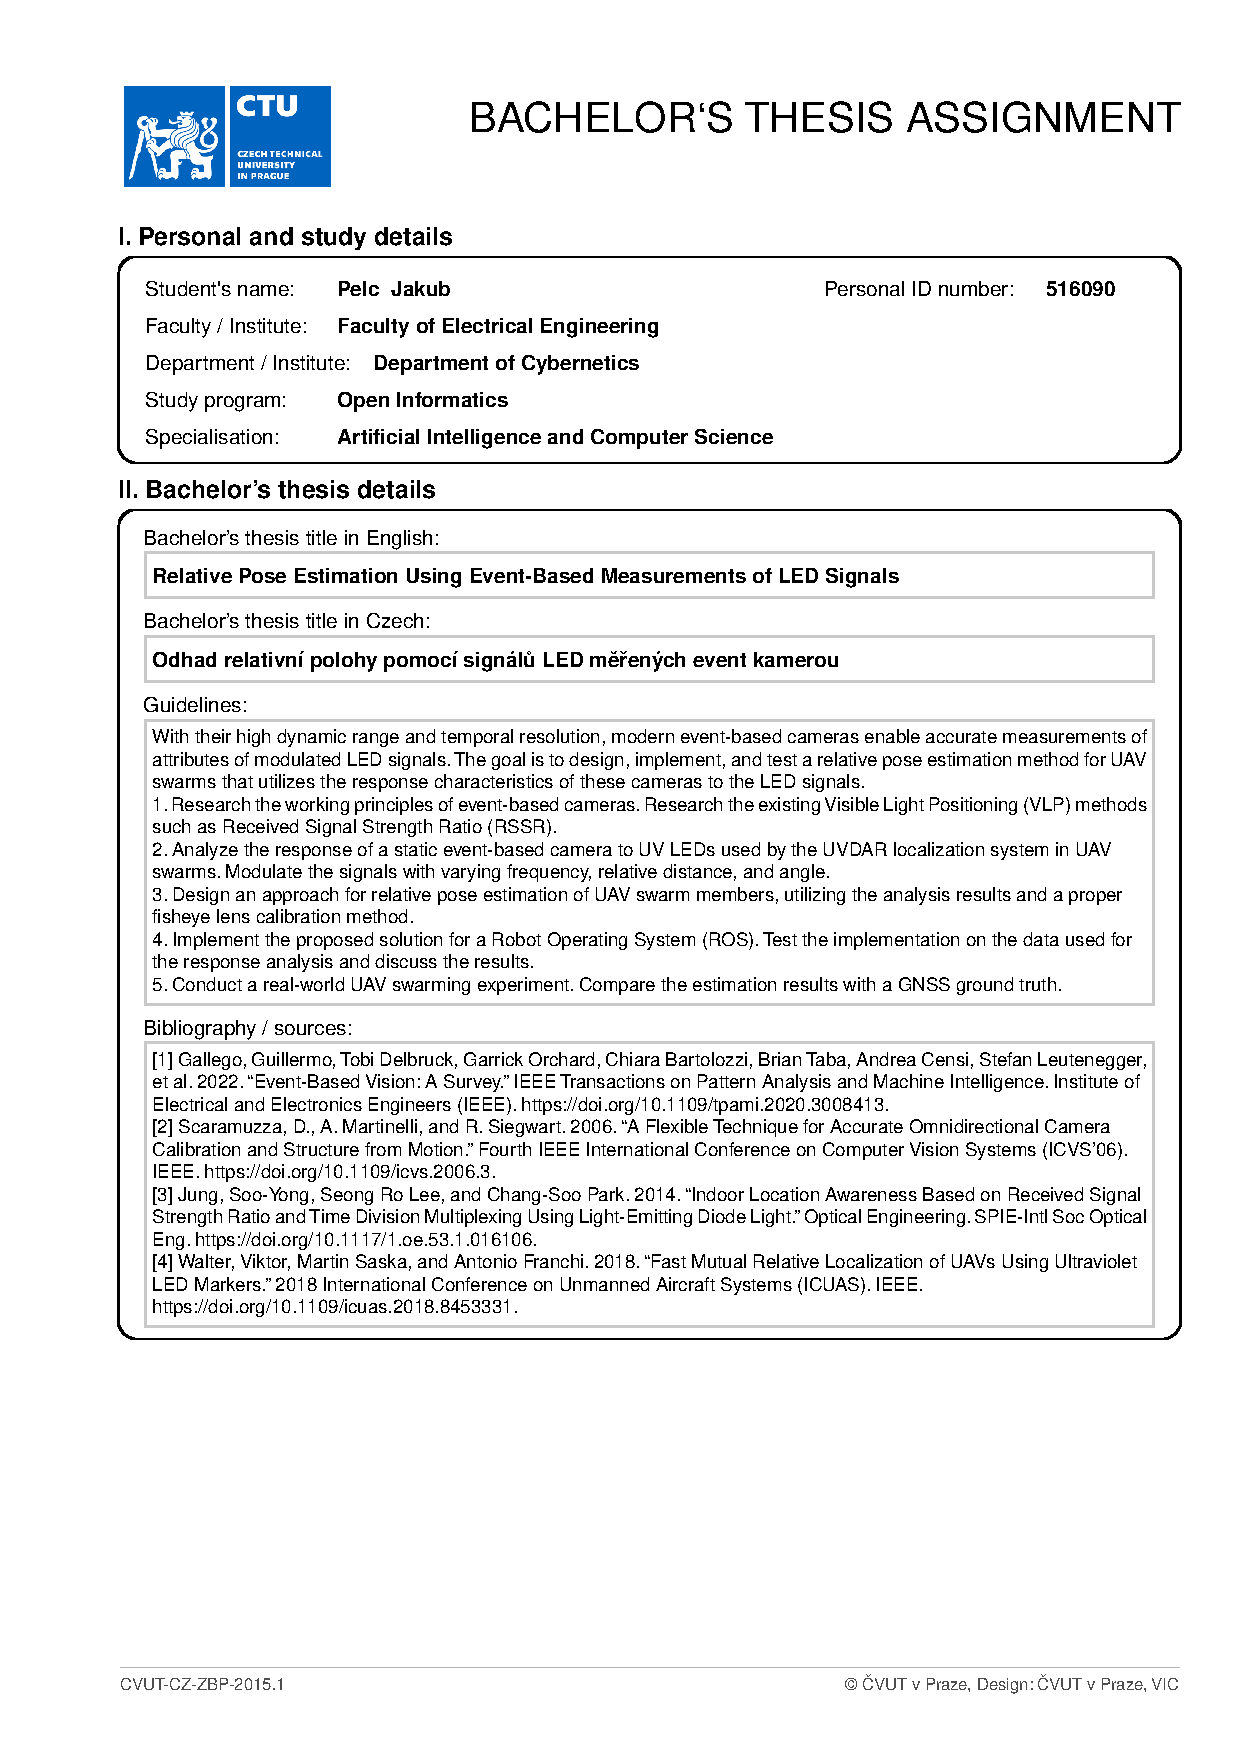
\includepdf{src/assignment.pdf}

%% --------------------------------------------------------------
%% |                         Declaration                        |
%% --------------------------------------------------------------

\conditionalClearPage

~\vfill{}

\section*{Declaration}
%\section*{Prohlášení autora práce}

I declare that presented work was developed independently, and that I have listed all sources of information used within, in accordance with the Methodical instructions for ob-serving ethical principles in preparation of university theses.
% Prohlašuji, že jsem předloženou práci vypracoval samostatně a že jsem uvedl veškeré použité informační zdroje v souladu s Metodickým pokynem o dodržování etických principů při přípravě vysokoškolských závěrečných prací.

\vspace{1.5cm}
~\\

Date .............................\hfill{}...............................................
% Dne.............................\hfill{}...............................................

\hfill{}~~~~~~~~~~~~~~~

\newpage{}


%% --------------------------------------------------------------
%% |                          Abstracts                         |
%% --------------------------------------------------------------

\conditionalClearPage

%!TEX root = ../main.tex

\begin{changemargin}{0.8cm}{0.8cm}

~\vfill{}

\section*{Abstract}
\vskip 0.5em
This thesis presents a way to estimate the relative pose of an object equipped with modulated light emitters
using an event-based camera as the sensor. Our approach begins by detecting and clustering the asynchronous events into blobs of
pixels, for which their centroids are computed. By associating these centroids with the known geometry of the light
emitters, the rotation and translation of the object is solved for via the Perspective-n-Point algorithm.
To ensure accurate measurements, a customized camera and lens calibration procedure is first performed, which
consists of a target with equally spaced diodes that provide bright reference points during calibration.
Experimental validation on static and dynamically moving quadrotors demonstrates an average localization accuracy of tens of
centimeters in stationary scenarios and a meters-level precision at large distances during active motion.

\vskip 1em

{\bf Keywords} \Keywords

\vskip 2.5cm

\end{changemargin}


\conditionalClearPage

%!TEX root = ../main.tex

\begin{changemargin}{0.8cm}{0.8cm}

~\vfill{}

\section*{Abstrakt}
\vskip 0.5em

\sloppy
Výzkum na poli autonomních bezpilotních prostředků (UAV) se stal významným oborem mobilní robotiky.

\vskip 1em

{\bf Klíčová slova} \KlicovaSlova

\vskip 2.5cm

\end{changemargin}


%% --------------------------------------------------------------
%% |                        Abbreviations                       |
%% --------------------------------------------------------------

\conditionalClearPage

\begin{changemargin}{0.8cm}{0.8cm}

~\vfill{}

\section*{Abbreviations}

% this will print only the used abbreviations
%!TEX root = ../main.tex

\begin{acronym}
  \acro{API}[API]{Application Programming Interface}
  \acro{CTU}[CTU]{Czech Technical University}
  \acro{DOF}[DOF]{degree-of-freedom}
  \acro{DVS}[DVS]{Dynamic Vision Sensors}
  \acro{FOV}[FOV]{Field of View}
  \acro{FPS}[FPS]{Frames Per Second}
  \acro{GNSS}[GNSS]{Global Navigation Satellite System}
  \acro{GPS}[GPS]{Global Positioning System}
  \acro{IMU}[IMU]{Inertial Measurement Unit}
  \acro{LED}[LED]{Light Emitting Diode}
  \acro{LKF}[LKF]{Linear Kalman Filter}
  \acro{LTI}[LTI]{Linear time-invariant}
  \acro{LiDAR}[LiDAR]{Light Detection and Ranging}
  \acro{MAV}[MAV]{Micro Aerial Vehicle}
  \acro{MPC}[MPC]{Model Predictive Control}
  \acro{MRS}[MRS]{Multi-robot Systems Group}
  \acro{P3P}[P3P]{Perspective-Three-Point}
  \acro{PnP}[PnP]{Perspective-n-Point}
  \acro{ROI}[ROI]{Region of Interest}
  \acro{ROS}[ROS]{Robot Operating System}
  \acro{RSSR}[RSSR]{Received Signal Strength Ratio}
  \acro{RTK}[RTK]{Real-time Kinematics}
  \acro{SLAM}[SLAM]{Simultaneous Localization And Mapping}
  \acro{TDOA}[TDOA]{Time Difference of Arrival}
  \acro{UAV}[UAV]{Unmanned Aerial Vehicle}
  \acro{UGV}[UGV]{Unmanned Ground Vehicle}
  \acro{UKF}[UKF]{Unscented Kalman Filter}
  \acro{UV}[UV]{Ultra Violet}
  \acro{VLP}[VLP]{Visible Light Positioning}
\end{acronym}


\vskip 2.5cm

\end{changemargin}

\conditionalClearPage

%% --------------------------------------------------------------
%% |                      Table of contents                     |
%% --------------------------------------------------------------

\tableofcontents

\conditionalClearPage

% set up the full page style with normal page numbering
\pagestyle{full}
\pagenumbering{arabic}

%% --------------------------------------------------------------
%% |            introduction (and working principles)           |
%% --------------------------------------------------------------

%!TEX root = ../main.tex

\chapter{Introduction\label{chap:introduction}}

The rapid advancement of \ac{UAV} swarms has intensified the demand for robust and scalable relative pose estimation methods.
Traditional solutions relying on \ac{GNSS} suffer from limitations in indoor environments, signal occlusion, and interference that arises from
multi-agent communication.
\ac{VLP} systems, which leverage modulated \ac{LED} signals and optical sensors, offer a promising alternative due to their immunity to radio
frequency interference and high precision.

However, conventional frame-based cameras used in \ac{VLP} systems struggle with motion blur, latency,
and dynamic range constraints. For example, under bright illumination, \ac{LED}s may not produce a sufficiently detectable signal,
which may lead to localization failure. In contrast, event-based cameras overcome these limitations by asynchronously detecting pixel-level
brightness changes, providing microsecond temporal resolution, high dynamic range, and minimal latency. These attributes make them ideal for
capturing high-frequency LED signals, even in challenging lighting conditions or during aggressive \ac{UAV} maneuvers in agile swarming applications.

\todo{maybe write more}

\section{Related works}
Recent advances in relative pose estimation for UAV swarming applications
have focused on GNSS-denied environments and the overcoming of limitations
the navigation faces in these environments.
%In GNSS-denied environments various techniques, including visual odometry, radio communication

Shiba et al. \cite{Shiba25cvprw} released E-VLC dataset for visible light communication, a dataset combining an event camera, a frame camera, and synchronized ground-truth poses in various recording conditions for modulated visible-\ac{LED} communication and localization tasks.

Ebmer et al. \cite{ebmer2023} proposed an event-based camera pipeline for real-time 6-\ac{DOF} pose estimation using visible active LED markers. Their system achieved a latency below \SI{0.5}{\milli\second}, with a mean tracking accuracy of \SI{34.5}{\milli\meter} (translation) and \SI{0.738}{\degree} (rotation). The detection mode showed higher errors, with mean values of \SI{64.9}{\milli\meter} and \SI{1.55}{\degree} for translation and rotation, respectively. Standard deviations were \SI{16.2}{\milli\meter} and \SI{0.146}{\degree} for tracking, but increased significantly to \SI{121}{\milli\meter} and \SI{5.12}{\degree} for detection. Maximum observed errors reached \SI{87.8}{\milli\meter} (tracking) and \SI{1.233}{\meter} (detection) in translation, and up to \SI{71.9}{\degree} in rotation during detection.

Gou et al. \cite{GOU2025328} proposed a hybrid framework fusing depth-sensor data and event-based camera streams in a joint random-optimization scheme to achieve robust camera tracking and dense reconstruction under fast motion for agile robotics tasks.

\section{Contributions}

In this thesis, we present a method for estimating the pose of a \ac{UAV} equipped with \ac{UV} \ac{LED} light sources as in the UVDAR system. \cite{walteruvdar}
These \ac{LED}s are modulated at select frequencies, which aids in their identification and also helps with their prevalence
on the scene observed by the camera. After the camera is properly calibrated and the LED source locations are identified, a Perspective-n-Point 
algorithm is used to estimate the location of the \ac{UAV} in the 3D space. This estimation is then compared with the ground truth positions obtained
from the \ac{GNSS}.

\section{Mathematical notation}

\todo{reword this if necessary}

The following mathemathical notation in \reftab{tab:mathematical_notation} is used, unless specified otherwise.

\begin{table*}[!h]
  \scriptsize
  \centering
  \noindent\rule{\textwidth}{0.5pt}
  \begin{tabular}{lll}
    $\mathbf{x}$, $\bm{\alpha}$ & vector, pseudo-vector, or tuple\\
    %$\mathbf{\hat{x}}$, $\bm{\hat{\omega}}$& unit vector or unit pseudo-vector\\
    %$\mathbf{\hat{e}}_1, \mathbf{\hat{e}}_2, \mathbf{\hat{e}}_3$ & elements of the \emph{standard basis} \\
    $\mathbf{X}$ & matrix \\
    $\mathbf{I}$ & identity matrix \\
    $\mathbf{R}$ & rotation matrix \\
    $\mathbf{t}$ & translation vector \\
    %$x = \mathbf{a}^\intercal\mathbf{b}$ & inner product of $\mathbf{a}$, $\mathbf{b}$ $\in \mathbb{R}^3$\\
    %$\mathbf{x} = \mathbf{a}\times\mathbf{b}$ & cross product of $\mathbf{a}$, $\mathbf{b}$ $\in \mathbb{R}^3$\\
    %$\mathbf{x} = \mathbf{a}\circ\mathbf{b}$ & element-wise product of $\mathbf{a}$, $\mathbf{b}$ $\in \mathbb{R}^3$ \\
    %$\mathbf{x}_{(n)}$ = $\mathbf{x}^\intercal\mathbf{\hat{e}}_n$ & $\mathrm{n}^{\mathrm{th}}$ vector element (row), $\mathbf{x}, \mathbf{e} \in \mathbb{R}^3$\\
    %$\mathbf{X}_{(a,b)}$ & matrix element, (row, column)\\
    %$x_{d}$ & $x_d$ is \emph{desired}, a reference\\
    %$\dot{x}, \ddot{x}, \dot{\ddot{x}}$, $\ddot{\ddot{x}}$ & ${1^{\mathrm{st}}}$, ${2^{\mathrm{nd}}}$, ${3^{\mathrm{rd}}}$, and ${4^{\mathrm{th}}}$ time derivative of $x$\\
    %$x_{[n]}$ & $x$ at the sample $n$ \\
    %$\mathbf{A}, \mathbf{B}, \mathbf{x}$ & LTI system matrix, input matrix and input vector\\
    \emph{SO(3)} & 3D special orthogonal group of rotations\\
    %\emph{SE(3)} & \emph{SO(3)}~$\times~\mathbb{R}^3$, special Euclidean group\\
    $\delta(t)$ & Dirac delta function \\
    $\operatorname{Conv}(\cdot)$ & convex hull of points \\
  \end{tabular}
  \noindent\rule{\textwidth}{0.5pt}
  \caption{Mathematical notation, nomenclature and notable symbols.}
  \label{tab:mathematical_notation}
\end{table*}

%{\tiny\todo{REMOVE THIS\section{Document Statistics}\wordcount}}

%% --------------------------------------------------------------
%% |                   Event camera response                    |
%% --------------------------------------------------------------

%!TEX root = ../main.tex

\chapter{Response of an event-based camera\label{chap:response}}

\section{Event-based cameras compared to frame-based cameras}

Traditional frame-based (sometimes called global shutter) cameras capture the scene as a sequence of still image frames at fixed intervals with fixed settings, providing a synchronous representation of the visual world. 
In terms of ease of use and the simplicity of the post-processing of data obtained from such cameras, they are wildly applicable across many fields.
A single frame obtained from a frame-based camera may be described by the following equation \refeq{eq:frame} \cite{scheerlinck2018event}
\begin{equation}
Y_j(\boldsymbol{p}) := \frac{1}{\epsilon} \int_{t_j - \epsilon}^{t_j} Y(\boldsymbol{p}, \tau) \mathrm{d} \tau, \quad j \in 1, 2, 3 ...
\label{eq:frame}
\end{equation}
where $Y(\boldsymbol{p}, t)$ denotes the irradiation intensity of a camera pixel at a specific time $t$, $t_j$ is the time-stamp of the image capture and $\epsilon$ is the exposure time.
As we can see, each frame is represented by a temporal average of irradiance over the exposure time $\epsilon$. Although this model simplifies image formation, it introduces artifacts such as motion blur, particularly when fast-moving objects are captured with an exposure time mismatched to their dynamics.

\ac{DVS} (or event-based cameras), are vision sensors that draw their inspiration from nature bio-receptors, where each pixel reacts
to the change of illumination in the scene. Each pixel individually recognizes the log intensity and compares it to the previously
recorded value. When a predefined threshold is crossed, this value is reset to the current one and a new event is generated. This event can be expressed as $e = \begin{bmatrix} x & y & \sigma & t \end{bmatrix}$, where $\begin{bmatrix} x & y \end{bmatrix}$
is the camera pixel coordinate, $\sigma$ is the polarity of change (where $\sigma = \pm 1$ for increasing or decreasing change, respectively) and $t$ is the timestamp of the event. \cite{gallego22event} \cite{scheerlinck2018event} We can model the single event as a Dirac-delta function $\delta(t)$ and can define an event stream
$e_i(\boldsymbol{p}, t)$ at a pixel $\boldsymbol{p}$ by \refeq{eq:event_eq} \cite{scheerlinck2018event}
\begin{equation}
e_i(\boldsymbol{p}, t) := \sigma_i^{\boldsymbol{p}} c \, \delta(t - t_i^{\boldsymbol{p}}), \ i \in 1, 2, 3 ...
\label{eq:event_eq}
\end{equation}
where $\sigma_i^{\boldsymbol{p}}$ is the polarity and $t_i^{\boldsymbol{p}}$ is the time-stamp of the $i$-th event at a pixel.
The magnitude $c$ is the contrast threshold, a preset constant (similar to exposure time in frame-based cameras), which defines a change in light intensity that is encoded by a singular event, at each pixel. Event-based cameras thus circumvent many common issues found in traditional frame-based cameras, such as the motion blur mentioned before. They offer significant advantages, including high dynamic range, low latency,
and energy efficiency.
This makes them perfect for the application of agile robotics,
where the fast response time is crucial (especially in UAV swarming situations). With their submillisecond response time,
event cameras can provide a significant advantage over traditional cameras in these applications.
However, they also come with some drawbacks, such as the need for a different approach to
data processing (images can be reconstructed from the event stream by simply integrating the events over time,
making the usage of normal vision algorithms possible, but it also goes against the main advantage of event cameras)
and the higher cost of the camera units themselves. \cite{gallego22event}

\section{Equipment used}

The event-based camera used in this thesis is the Prophesee EVK4\footnote{Prophesee EVK4 website: \url{https://www.prophesee.ai/event-camera-evk4/}.}, featuring a resolution of $1280 \times 720$ pixels, with a maximum frame rate equivalent of $10.000 \text{FPS}$ and a 120 dB dynamic range.
A fish eye lens with an integrated UV filter was used during the measurements to target the specific wavelength of the LEDs
that are used on the \ac{UAV}s. The \ac{UAV} used for measurements was a unit from the \ac{MRS} UVDAR system, with \ac{UV} \ac{LED} light sources,
mounted at each arm of the \ac{UAV}, which are used for localization and communication purposes.
Both can be seen in \reffig{fig:uavcam}.

\begin{figure}[H]
	\centering
	\subfloat[The event-based camera EVK4 from Prophesee with a fish eye lens.] {
	  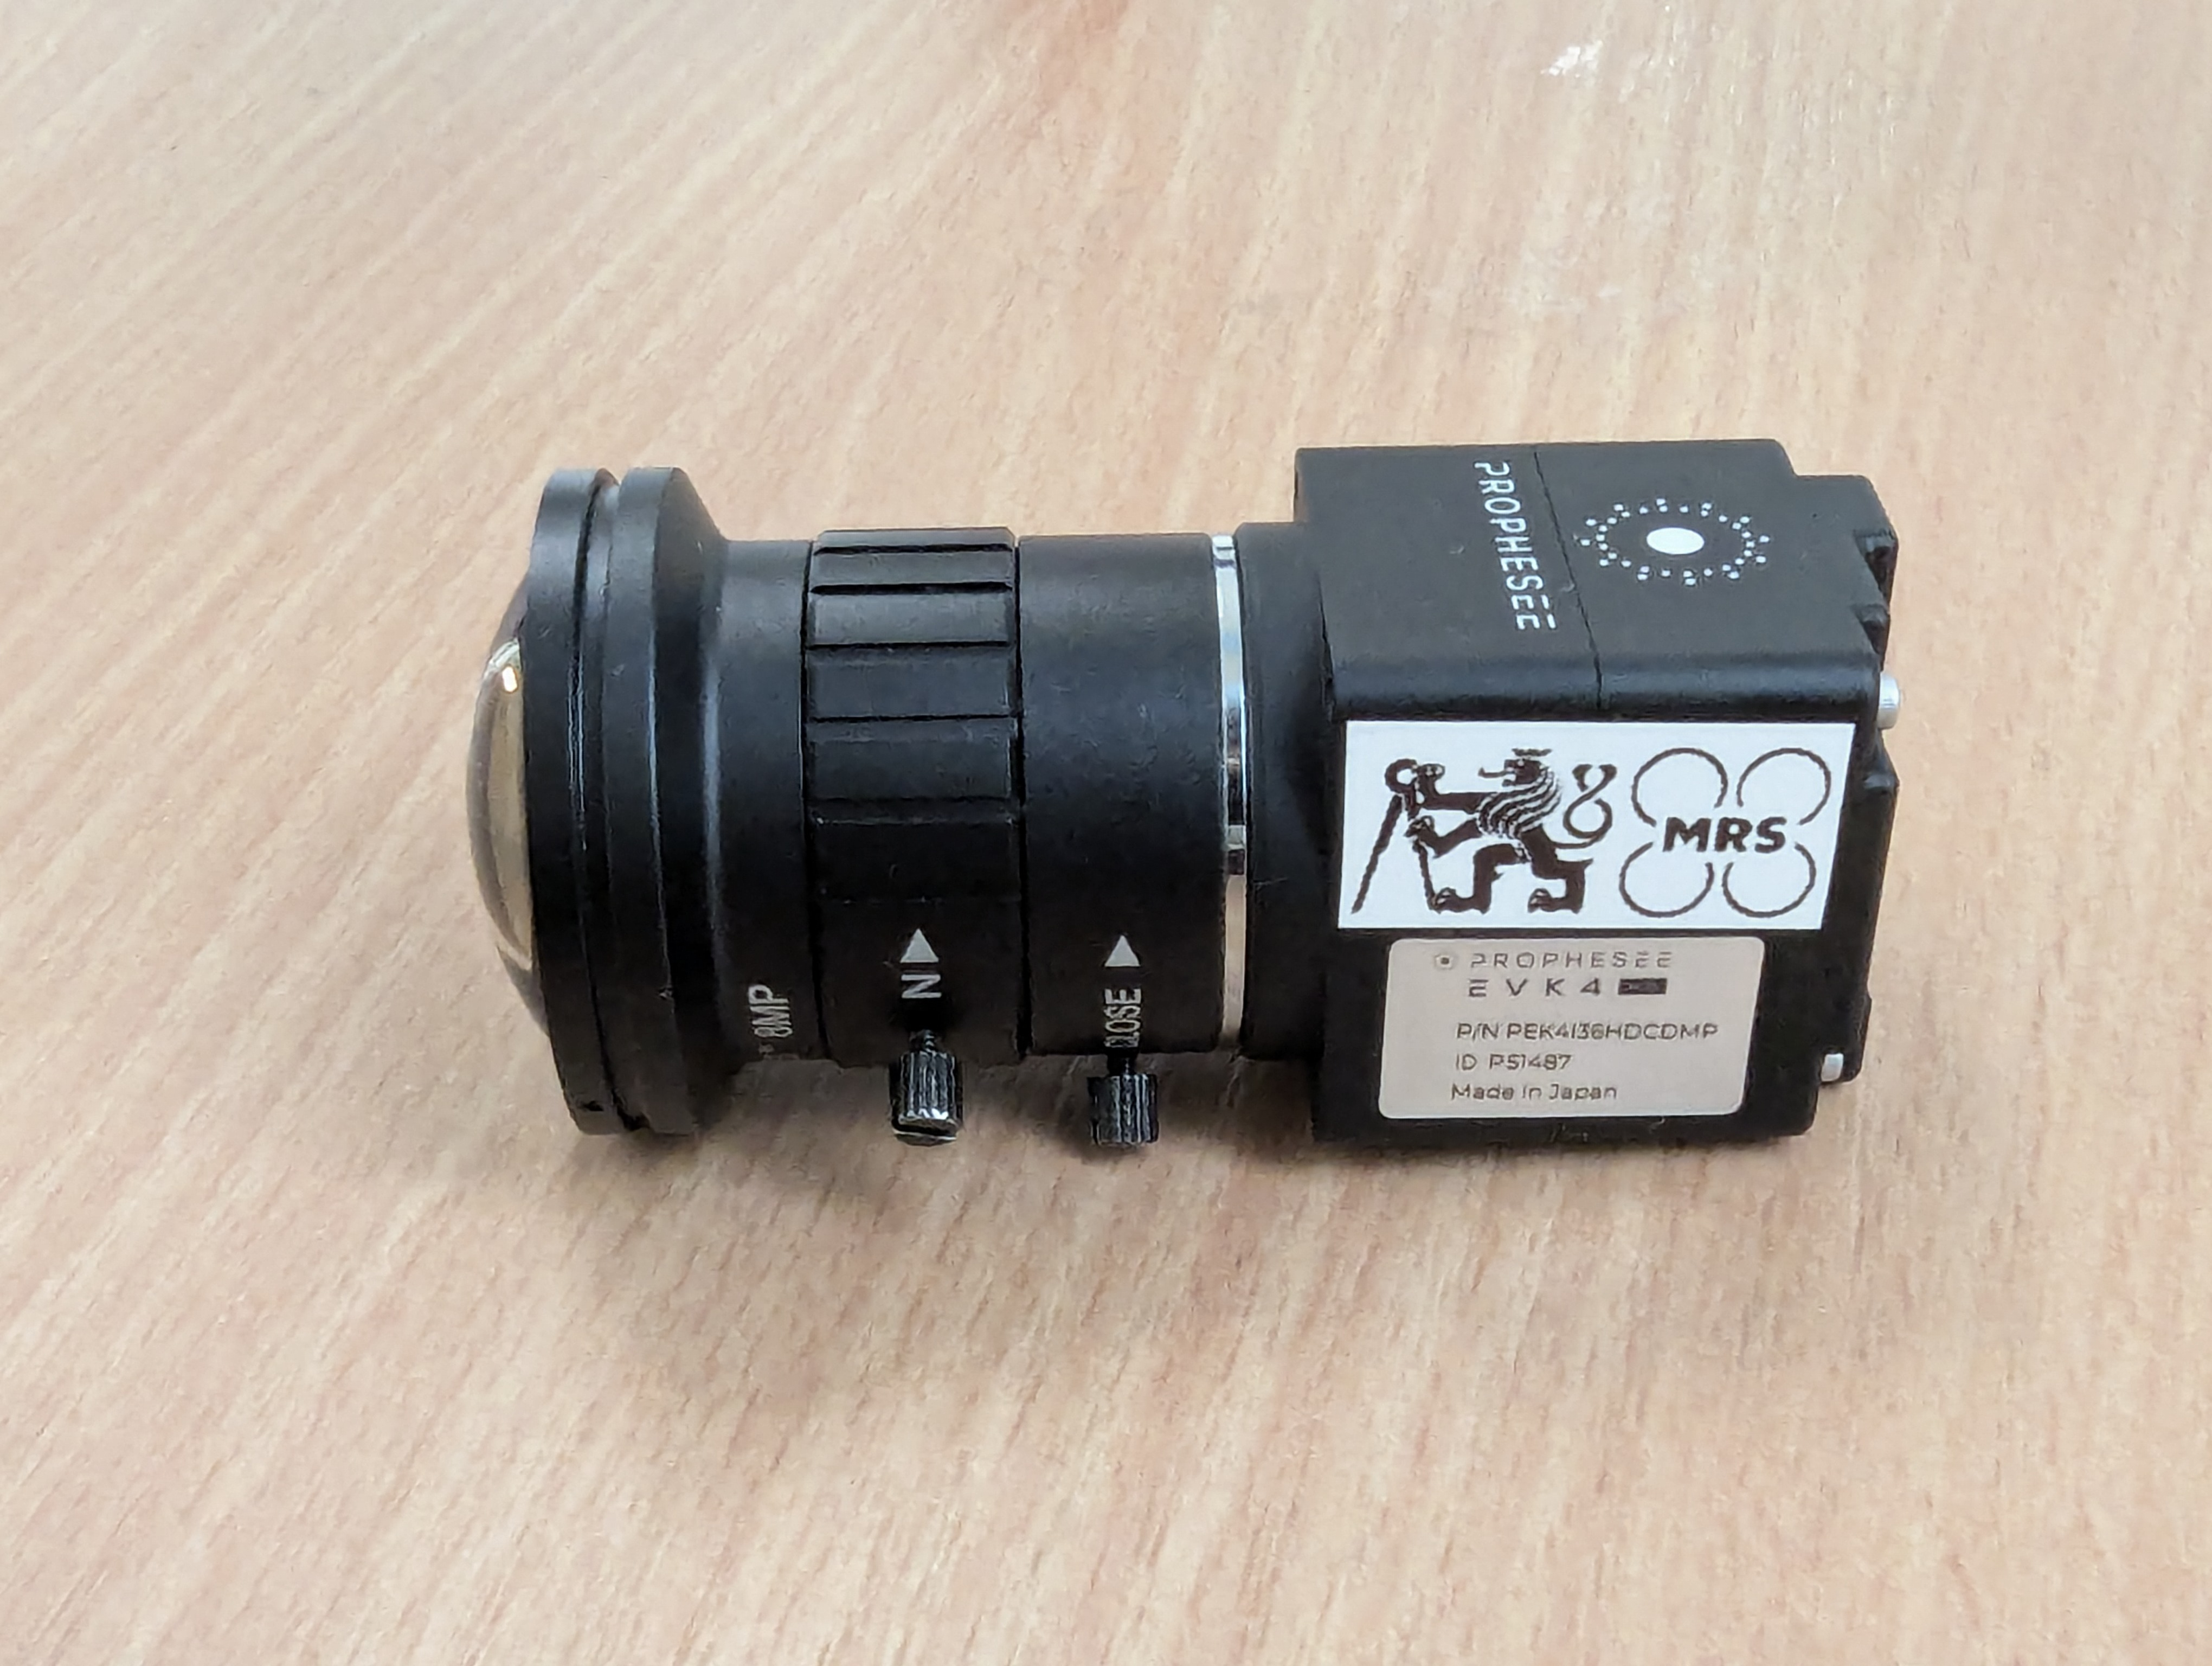
\includegraphics[width=0.5\textwidth]{./fig/photos/evk4.jpg}
	  \label{fig:evk4}
	}
	\subfloat[MRS UVDAR UAV unit] {
	  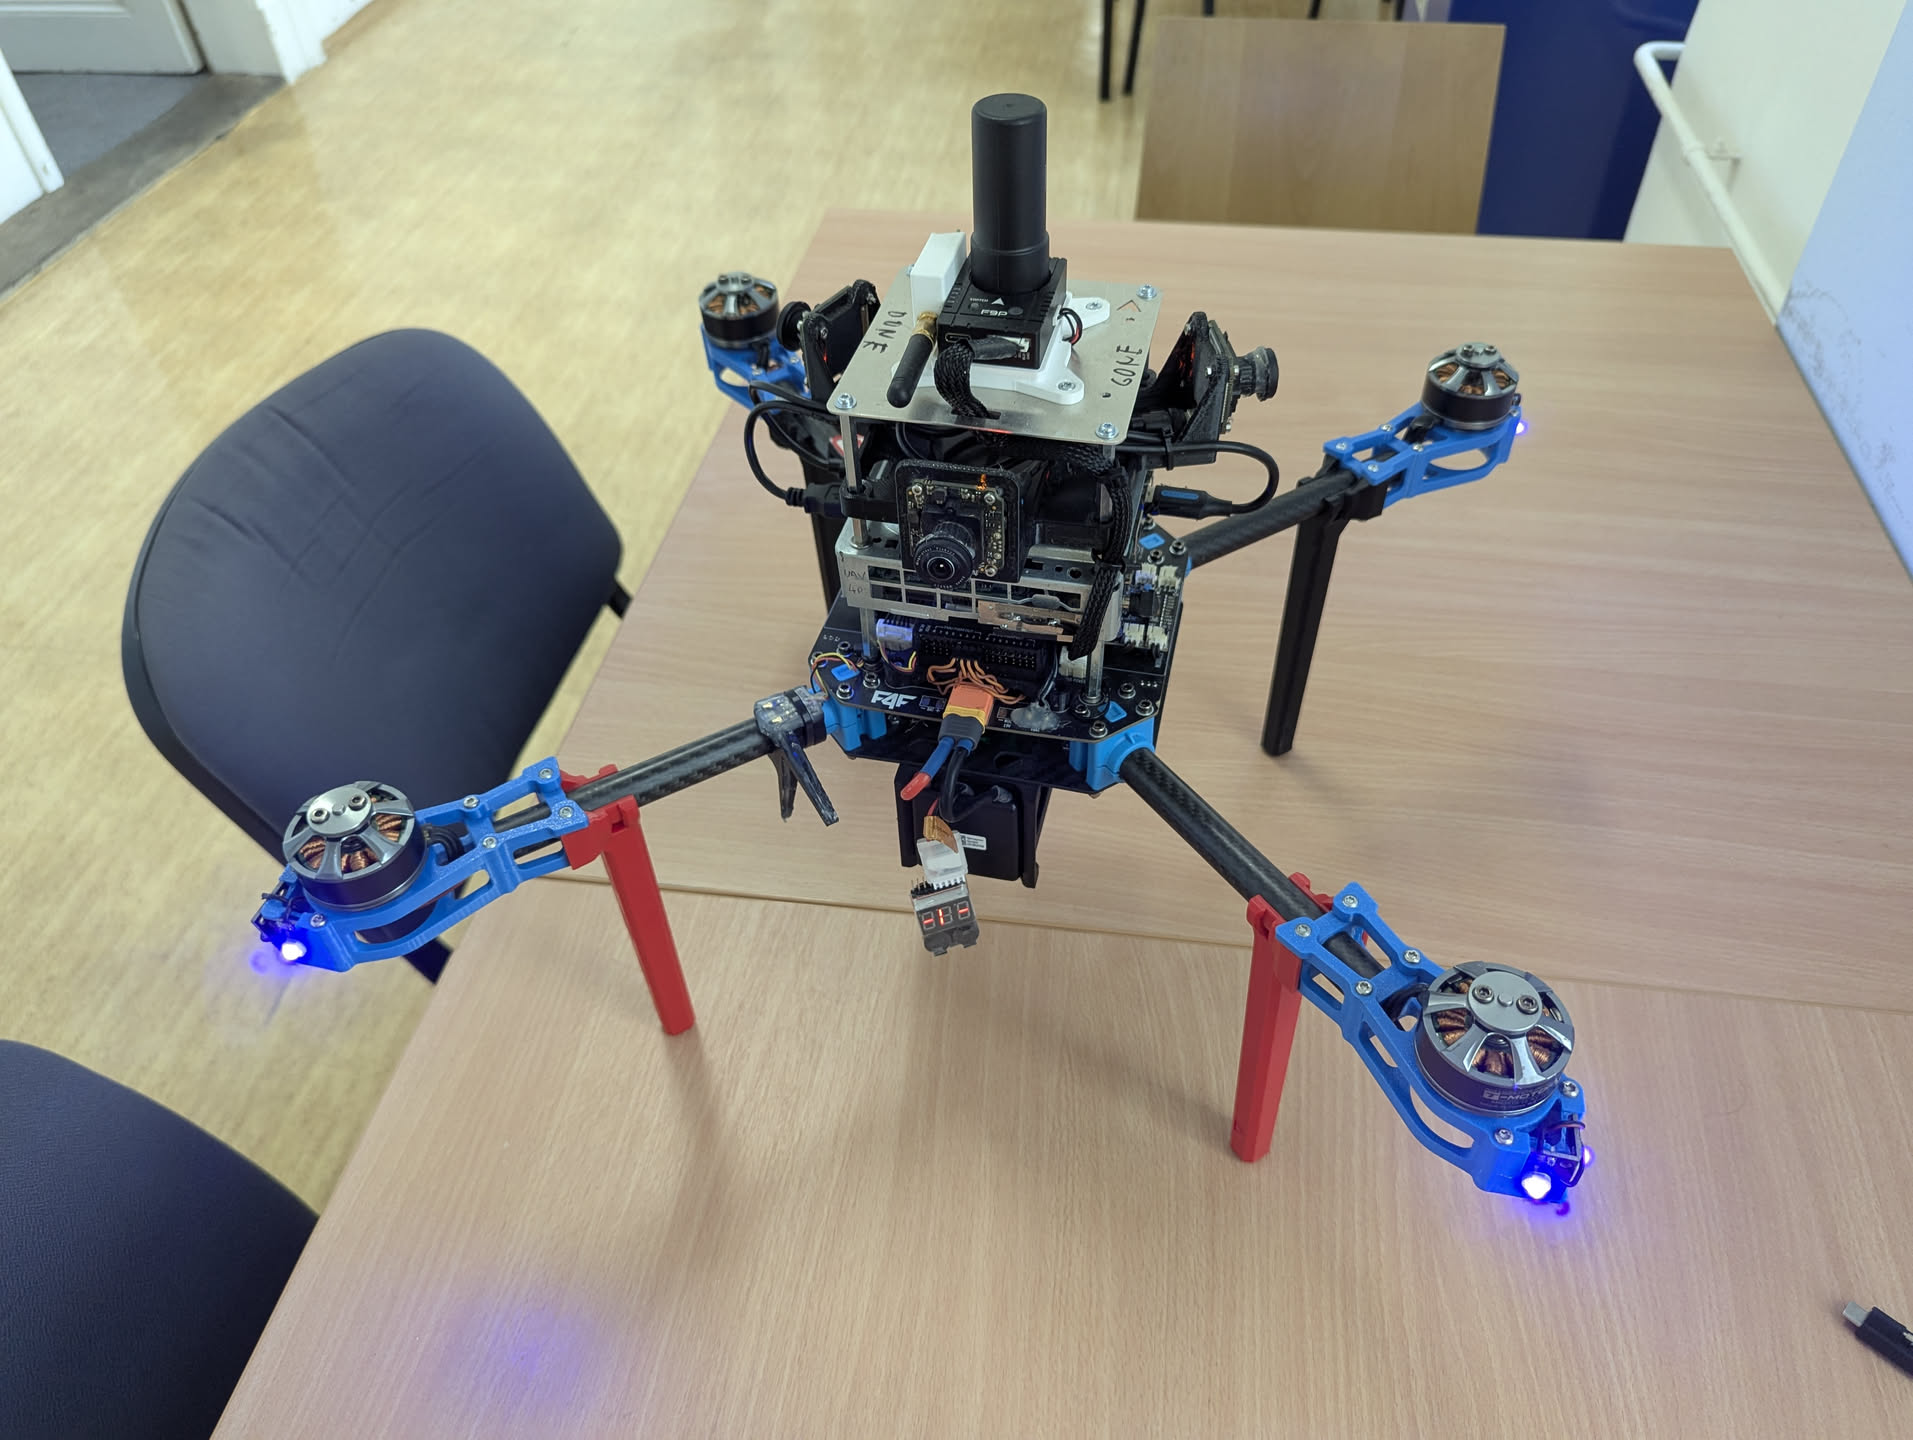
\includegraphics[width=0.5\textwidth]{./fig/photos/uav1.jpeg}
	  \label{fig:uav1}
	}
	\caption{
  An event-based camera with a fish eye lens can be seen on \reffig{fig:evk4}, which was used to measure the UV LEDs mounted on the UAV unit from the MRS UVDAR system as seen on \reffig{fig:uav1}.
  }
	\label{fig:uavcam}
\end{figure}

\section{Data collection}

The data have been collected on several occasions by measuring a stationary UAV at various distances and rotations from the camera.
Each UAV is equipped with 8 UV LEDs, with 2 LEDs on each arm of the UAV. Each of the LEDs can be individually controlled
and can be set to various sequences of blinking, and a common modulation frequency can be set for all LEDs.

\subsection{Initial measurements}

The initial measurements were made by securing the event camera on a tripod and placing the UAV at distances ranging from
$0.5$ to $2.5$ meters. The LEDs were set to blink at a frequency in the range of $1$ to $30$ kHz. No \ac{ROI} was set
and the whole visible area was recorded during the testing.

This first experiment proved to be rather inefficient as the LEDs need to be isolated from each other's influence, which
was not done properly at this time. This problem is solvable in the post-processing, by filtering out the events
by using an ROI filter (it is possible to filter the events by finding bounding boxes
that encapsulate light sources, but on a more complex scene this approach becomes relatively hard).
The other issue turned out to be the reflections of surrounding objects (as seen in \reffig{fig:meas1}), which caused
another source of unwanted events in the recording, which may in turn confuse some blob detection methods.

\begin{figure}[H]
	\centering
	\subfloat[An event-camera view of the UAV with UV LEDs.] {
	  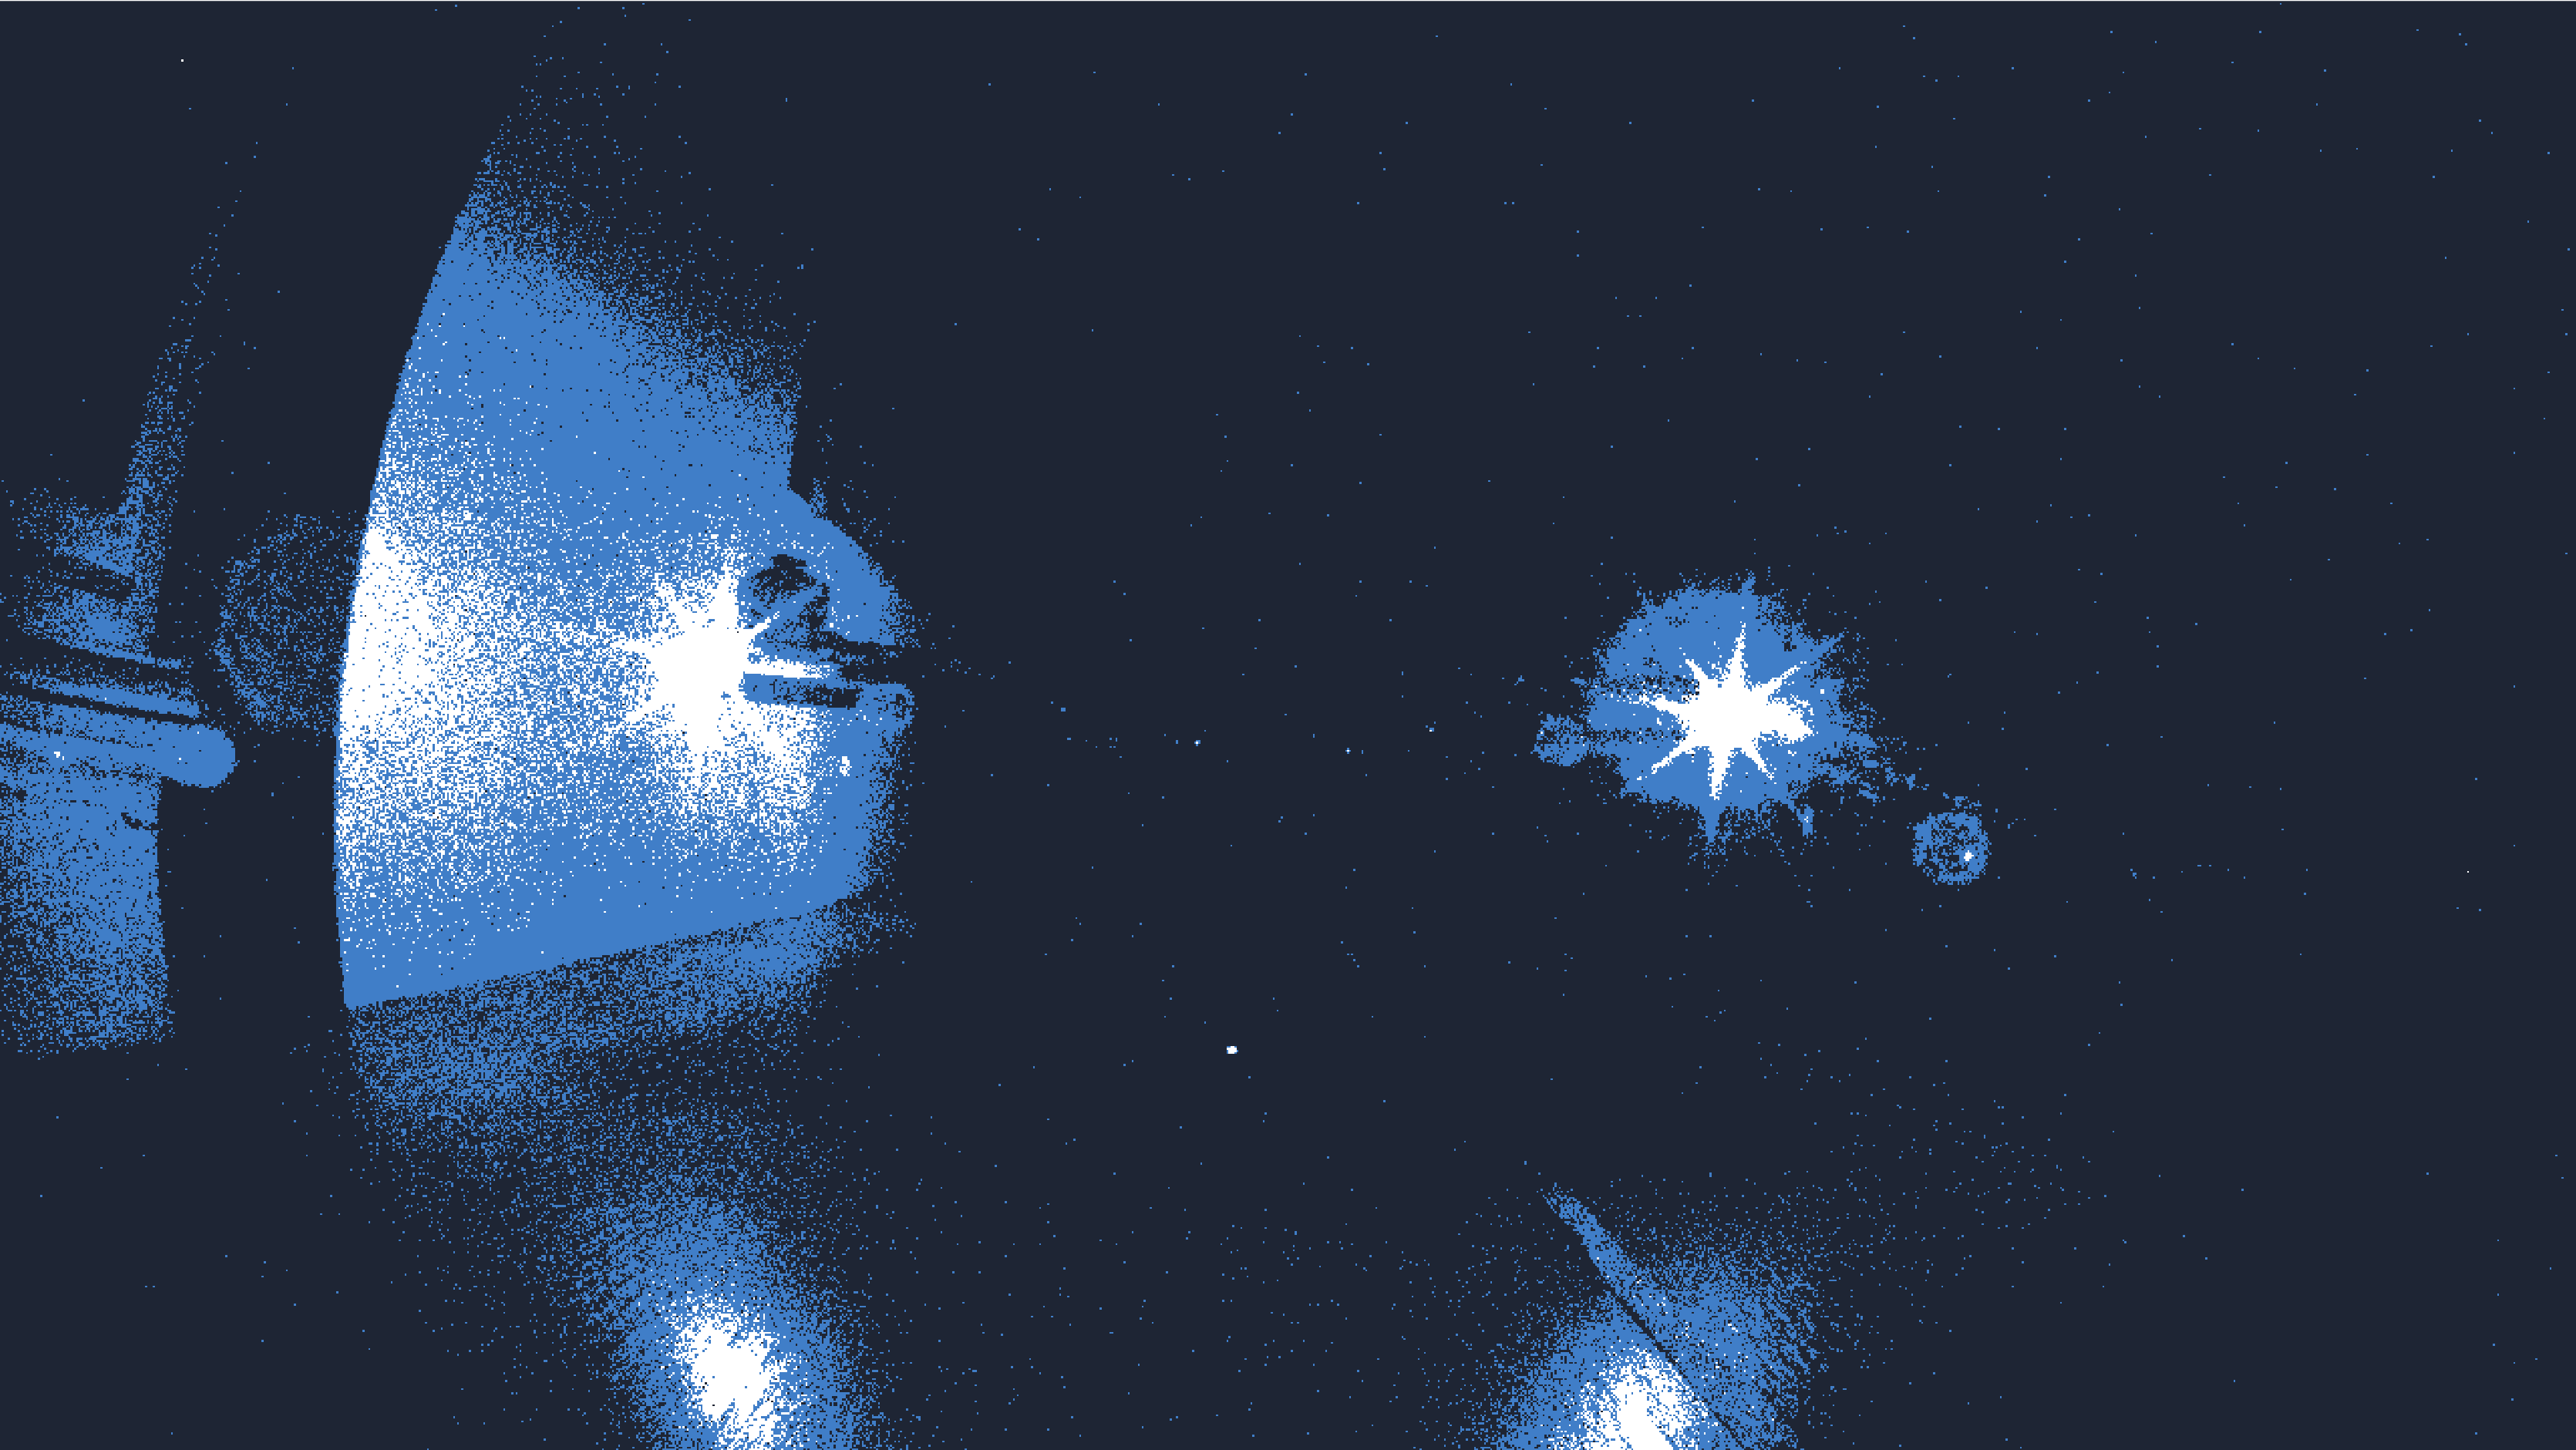
\includegraphics[width=0.5\textwidth]{./fig/photos/meas1.png}
	  \label{fig:meas1_e}
	}
	\subfloat[View of the experiment setup.] {
	  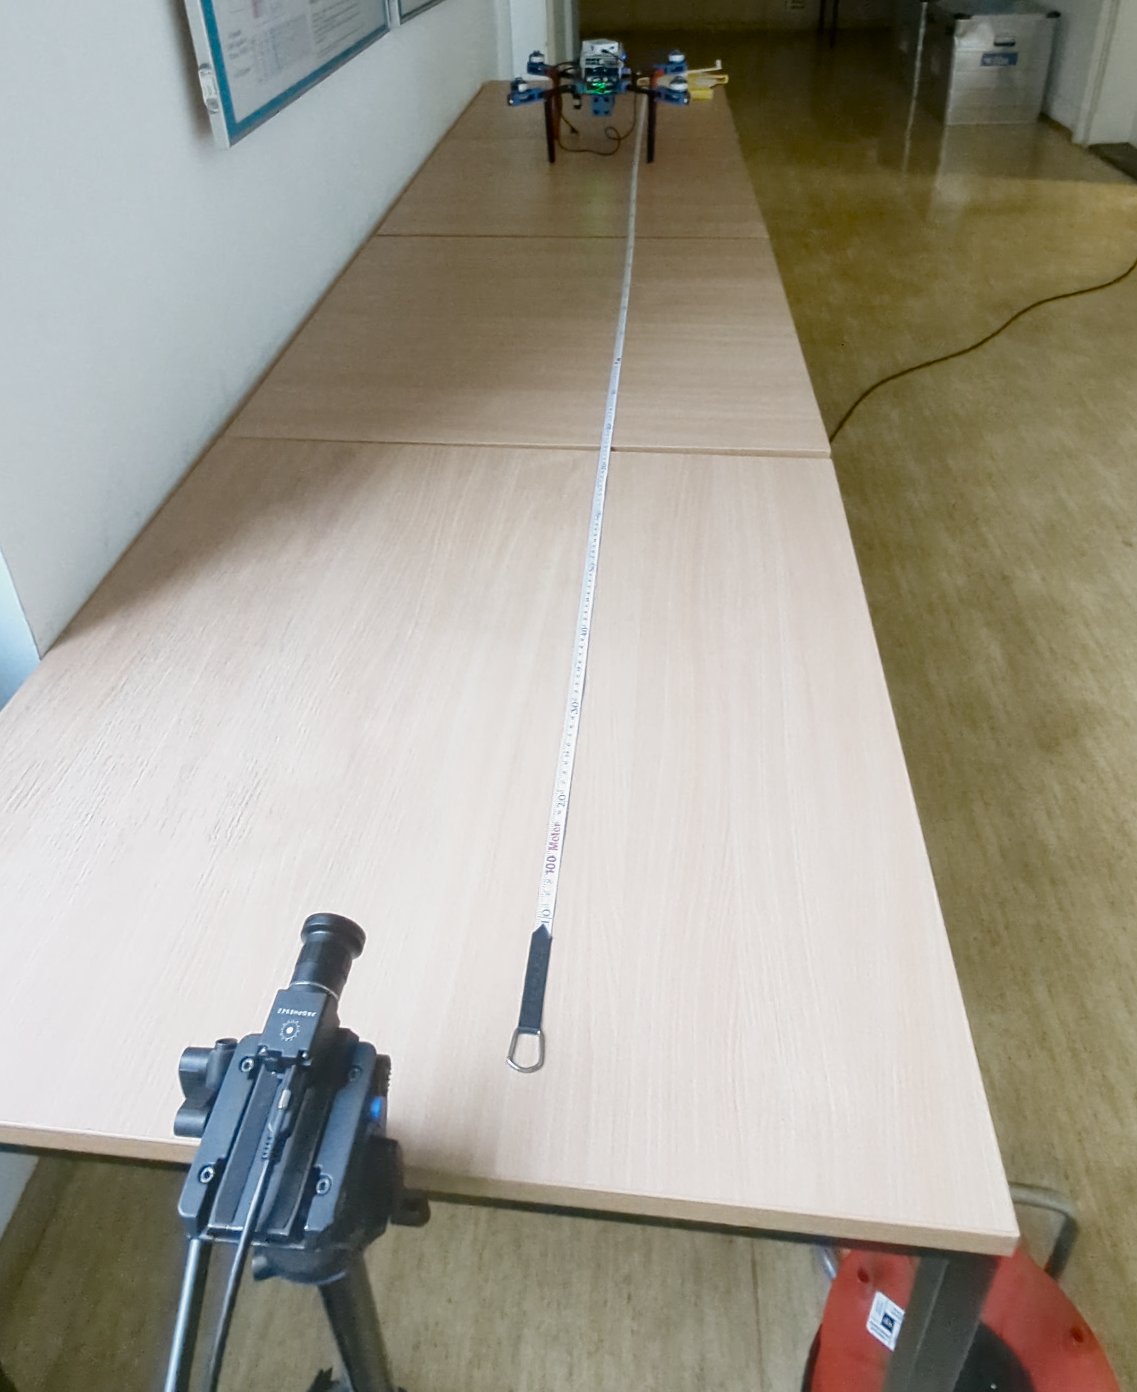
\includegraphics[width=0.5\textwidth]{./fig/photos/meas1_c.png}
	  \label{fig:meas1_c}
	}
	\caption{
  The setup for measuring the event-camera response with a EVK4 camera. Visible reflections from a wall can be seen on \reffig{fig:meas1}. The setup is shown on \reffig{fig:meas1_c}.
  }
	\label{fig:meas1}
\end{figure}


\subsection{Distance - frequency influence}

In the following measurements, we consider only one source of light as the whole end of the arm of the UAV (with 2 UV LEDs). Other arm light sources were turned off during the measurements.
Measurements were done on areas isolated by ROI filter directly in Metavision Studio, events were collected only on one select area around the light source, with the
rest of the events being discarded.
This time, the position of the UAV was fixed relative to the camera on a blank background. The camera was placed on a tripod
and moved in increments of $0.2$ meters, starting from $1$ meter and ending at $3$ meters, with additional measurements made
at $4$ and $5$ meters.
The frequency range of the LED modulation was set in a range of $10$ Hz to $30$ kHz, with the blinking sequence set to \texttt{0, 1}.

\subsection{Rotation angle influence}

In addition to distance and frequency influence, the rotation angle influence also needs to be considered, to
verify the emitting characteristics of the light sources - if they can or cannot be considered lambertian.
The UAV was rotated by increments of $45$ degrees relative to the event camera, at distances of $0.5$, $1$ and $2$ meters,
with frequencies ranging from $10$ Hz to $10$ kHz and the blinking sequence was set to \texttt{0, 1}.

\subsection{RSSR Data collection}

TODO: Rewrite this section

Another dataset was collected for the application of \ac{RSSR} \cite{sooyongrssr}, which we analyze more in \refchap{chap:rssr}.
The data includes calibration data, which is necessary for the optical system parameter estimation. This calibration is done by
recording a video using a calibration lattice of LEDs with known spacing, and observing the pattern distortion in the
resulting video.
The UAV was placed at increasing distances and various angles relative to the event camera, with the LEDs blinking at frequencies different from
each other. 
The blinking sequences were set to the following values:
\begin{lstlisting}
	led_1 = [0, 0, 0, 0, 0, 0, 0, 0, 1, 1, 1, 1, 1, 1, 1, 1]
	led_2 = [0, 0, 0, 0, 1, 1, 1, 1, 0, 0, 0, 0, 1, 1, 1, 1]
	led_3 = [0, 0, 1, 1, 0, 0, 1, 1, 0, 0, 1, 1, 0, 0, 1, 1]
	led_4 = [0, 1, 0, 1, 0, 1, 0, 1, 0, 1, 0, 1, 0, 1, 0, 1]
\end{lstlisting}
with a common modulation frequency of $250$ Hz.
This allows for the measurement of the ratio
%explain why to use the ratio, not the absolute value
\footnote{Using the absolute value of the LED power is not suitable, as it also depends of the camera settings, surrounding
environment and other factors. Finding such ratio (or property) that stays constant is crucial for correct distance estimation.}
between the responses for each of the LEDs, which is necessary
for the estimation of the UAV position using RSSR.

\section{Event response data processing}

The event-based camera response data was analyzed using Python in a Jupyter notebook
\footnote{Source code is available at: \url{https://github.com/kubakubakuba/mrs-uvdar-distance-estimator/blob/main/main.ipynb}},
with libraries from Metavision SDK\footnote{Metavision SDK Docs: \url{https://docs.prophesee.ai/stable/index.html}}.

TODO: MAYBE REMOVE THIS

The notebook is divided into sections that represent several datasets that were recorded during the measurements.
The precomputed average number of events with standard deviation is stored in the \texttt{. npz} files in the \texttt{./data} directory to speed up the visualization process.

\subsection{Distance - frequency influence}

The distance frequency dataset has recordings of the UAV placed in front of the camera at distances $\mathcal{D}$ and with one LED being modulated
at frequencies $\mathcal{F}$ \footnote{The frequencies represented in this list are the actual frequencies sent to the UVDAR unit. The preserved frequencies
are half of the values in this list - UVDAR interprets the frequency with a reference to the length of the sequence (here the sequence being \texttt{[0, 1]}).}. To minimize interference, only one LED was active during each recording, enabling isolated characterization of the diode’s response. The tested ranges were:
\[
\mathcal{F} = \{10, 25, 50, 100, 250, 500, 1000, 2500, 5000, 10000, 20000, 30000\} \, \text{Hz},
\]
\[
\mathcal{D} = \{1.0 + 0.2k \mid k \in \{0, \dots, 10\}\} \cup \{4.0, 5.0\} \, \text{m}.
\]
%\begin{lstlisting}
%frequencies_Hz = [10, 25, 50, 100, 250, 500, 1000, 2500, 5000, 10000, 20000, 30000]
%distances_m = [1.0, 1.2, 1.4, 1.6, 1.8, 2.0, 2.2, 2.4, 2.6, 2.8, 3.0, 4.0, 5.0]
%\end{lstlisting}
We can load the dataset into a matrix representing the distances and frequencies, then load a select number of events from each recording.
The data is then resampled into a 1D array by summing polarities over a selected bin width
\footnote{The bin width should be adjusted appropriately, as the farther the event camera is from the source, the fewer events are generated.}.
Peaks in this signal are then analyzed by SciPy's \texttt{findpeaks} function,
and the average number of events with the standard deviation is calculated for each frequency and distance.

We can see the influence of distance and frequency on the average number of events in \reffig{fig:dist} and \reffig{fig:freqs}, respectively. The data show a decreasing trend of the average number of events
with the increase of distance or frequency. The drop related to the distance can be explained by the perceived decrease in the intensity of the light source with increasing distance. With an increasing frequency, the camera cannot capture
all the changes that are generated by the light source. On very high frequencies and distances, the camera is not able
to detect any real events at all, as there is more noise generated by the camera itself at this point. This can be observed
at \reffig{fig:dist_2} with a frequency of $30$ kHz at $3$ meters.
If we now select one frequency and try to fit it with a curve,
we can see that the data can be approximated with a rational or exponential function, as shown in \reffig{fig:fit1}.
The best fit without being too complex is the inverse square law, which can be expressed as
\begin{equation}
	\text{intensity} \propto \frac{1}{\text{distance}^2}
\end{equation}

\begin{figure}[H]
	\centering
	\subfloat[Influence of distance on the average number of events.] {
	  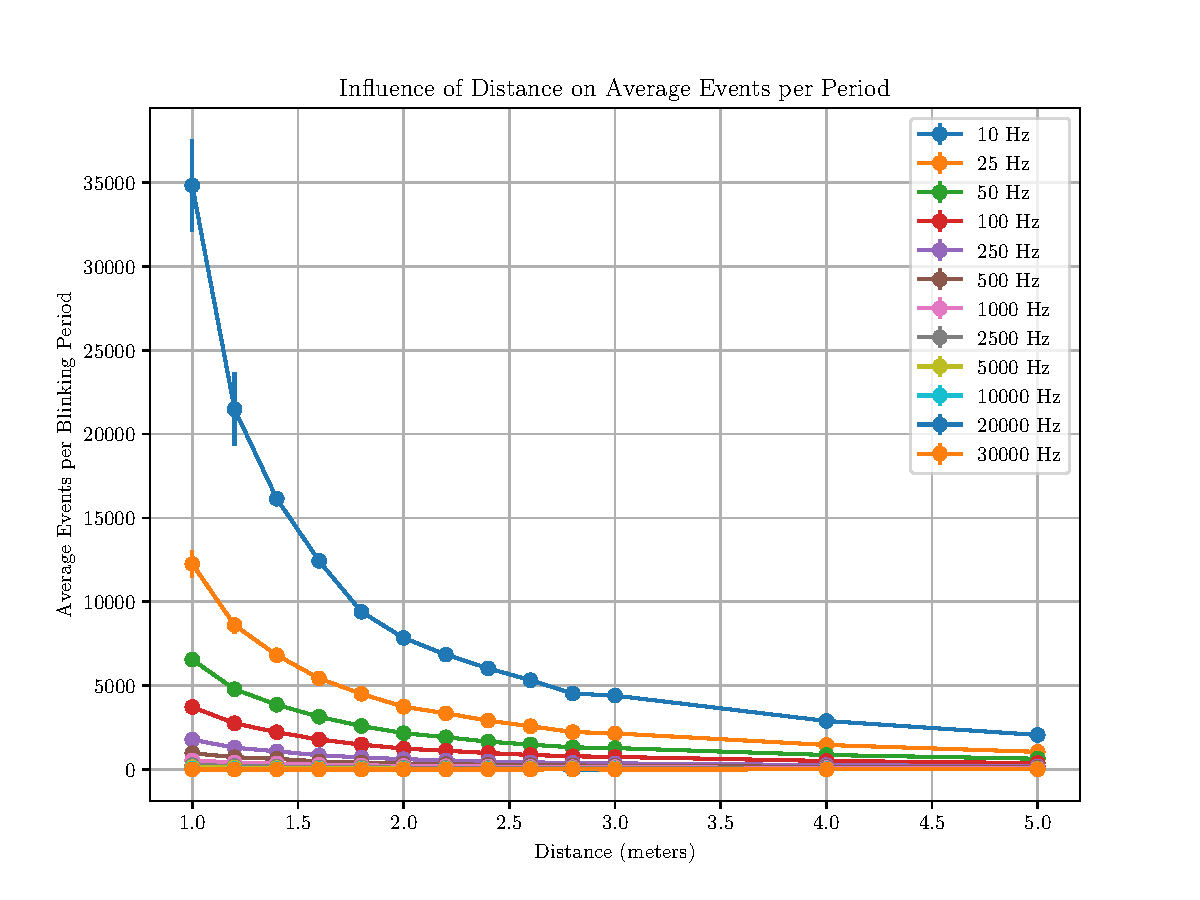
\includegraphics[width=0.5\textwidth]{./fig/semestral/dist.pdf}
	  \label{fig:dist_1}
	}
	\subfloat[Influence of distance on the log of average number of events.] {
	  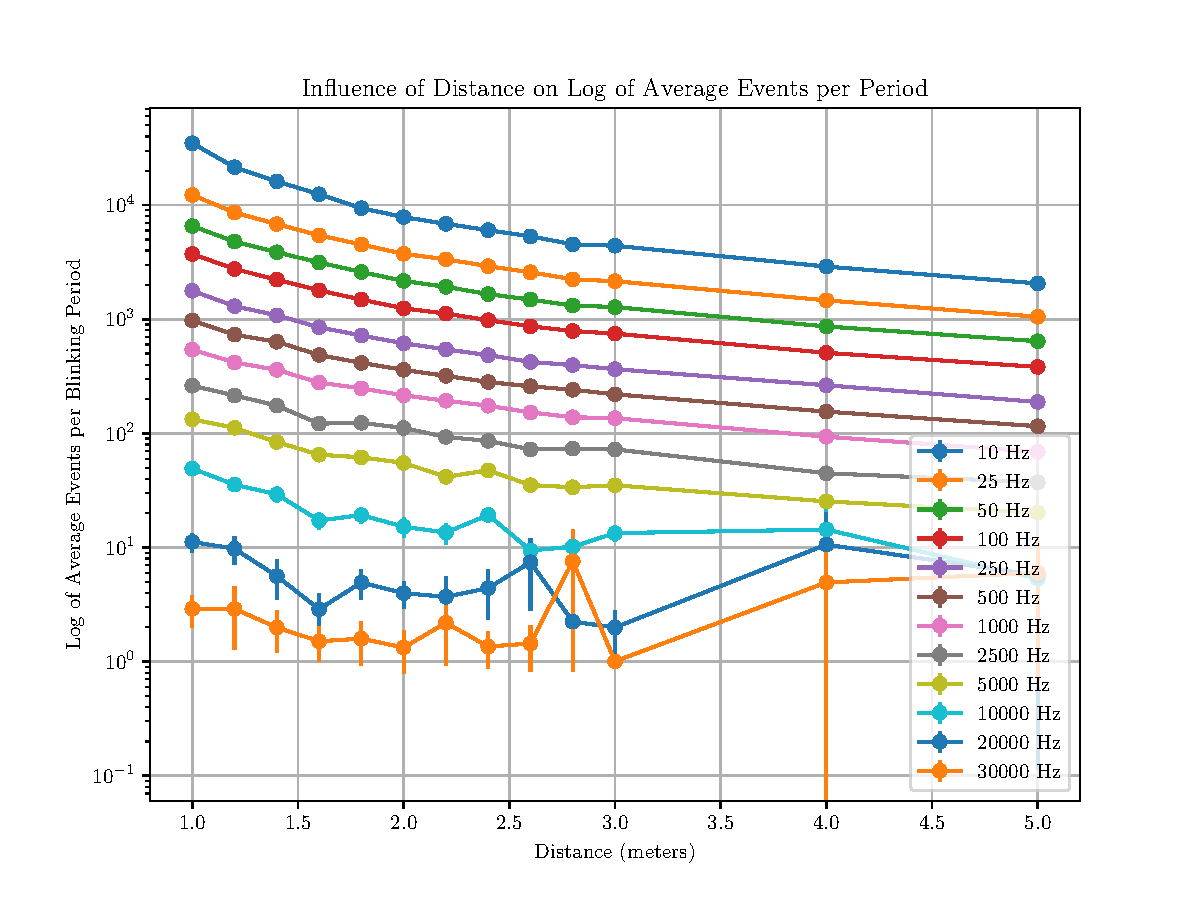
\includegraphics[width=0.5\textwidth]{./fig/semestral/distlog.pdf}
	  \label{fig:dist_2}
	}
	\caption{
  The influence of distance on the average number of events with the UAV rotated 0 degrees relative to the event camera on \reffig{fig:dist_1}, and with the log of the average number of events on \reffig{fig:dist_2}.
  }
	\label{fig:dist}
\end{figure}
\begin{figure}[H]
	\centering
	\subfloat[Influence of frequency on the average number of events.] {
	  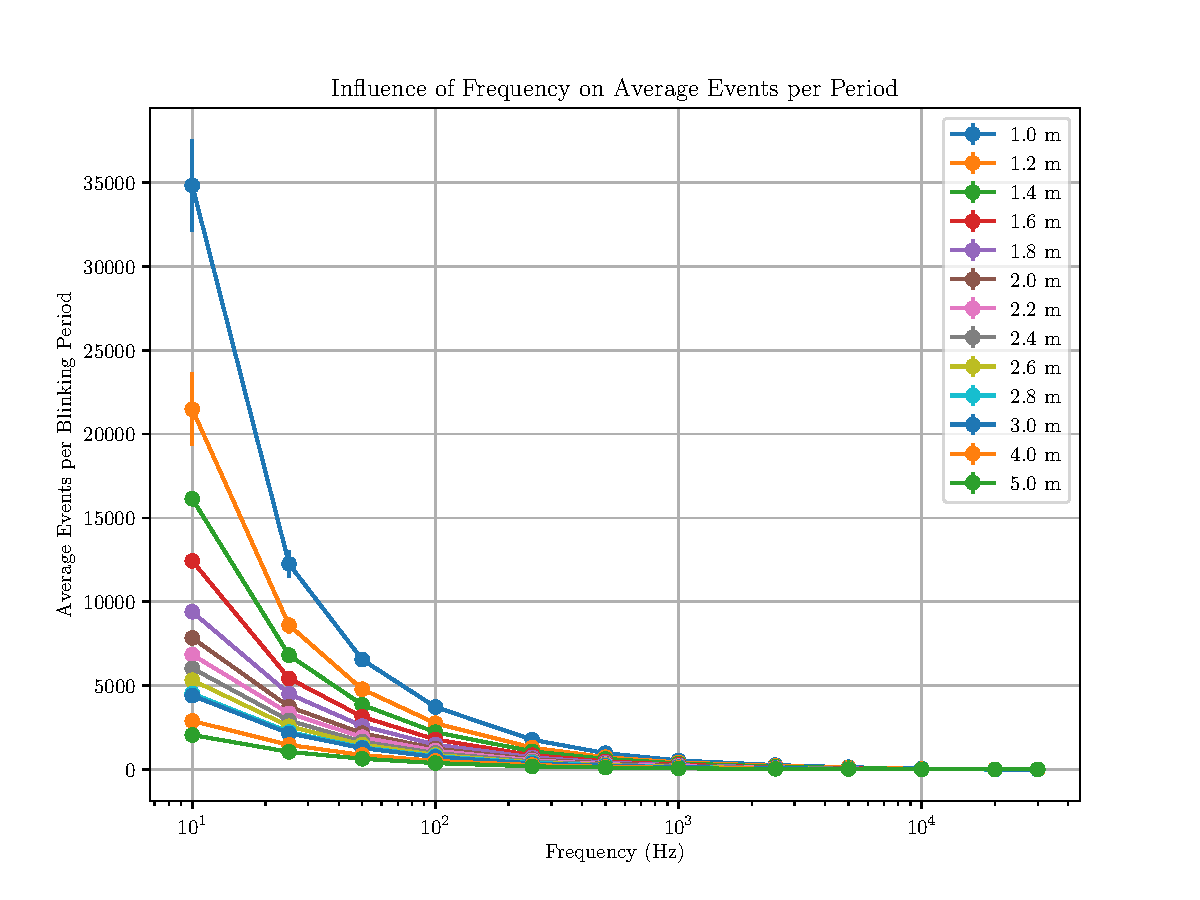
\includegraphics[width=0.5\textwidth]{./fig/semestral/freq.pdf}
	  \label{fig:freqs_1}
	}
	\subfloat[Influence of frequency on the log of average number of events.] {
	  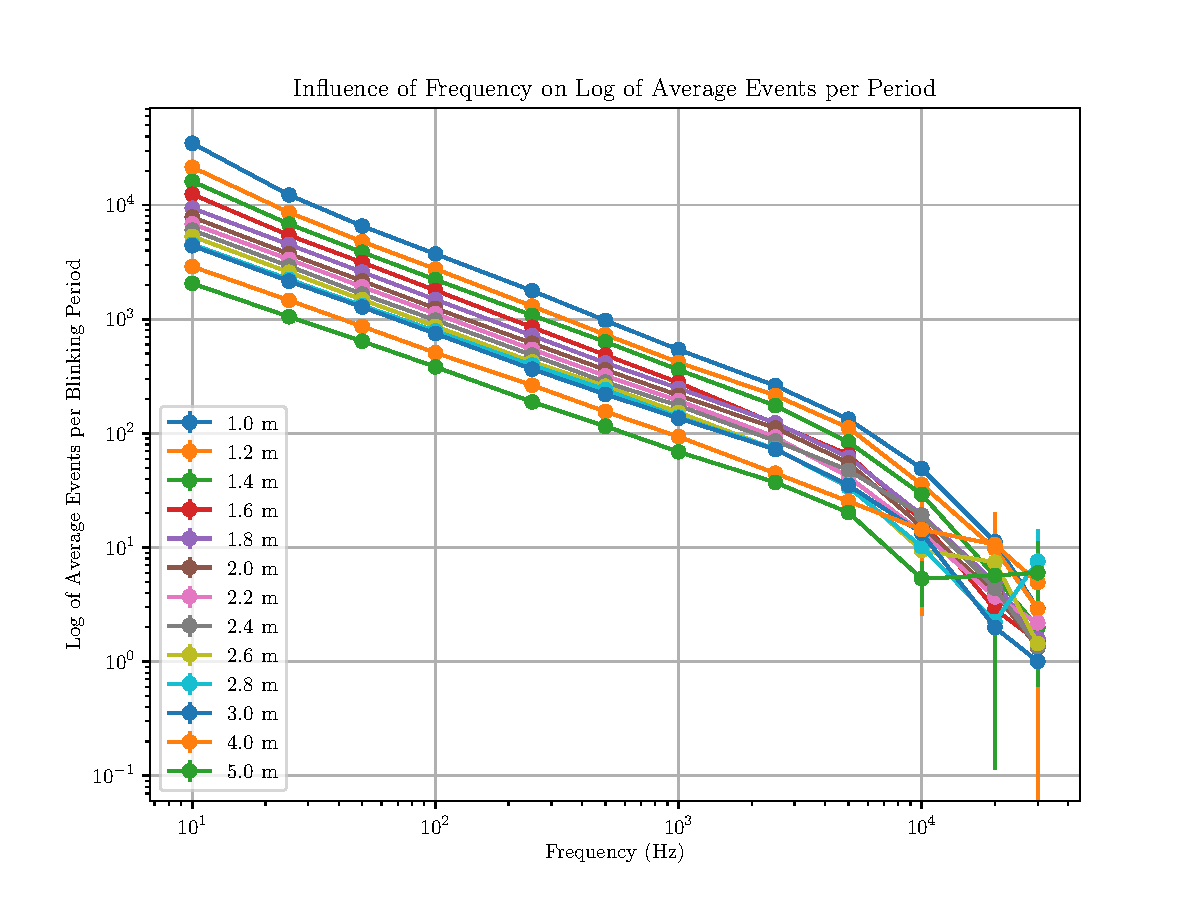
\includegraphics[width=0.5\textwidth]{./fig/semestral/freqlog.pdf}
	  \label{fig:freqs_2}
	}
	\caption{
  The influence of frequency on the average number of events with the UAV rotated 0 degrees relative to the event camera on \reffig{fig:freqs_1}, and with the log of the average number of events on \reffig{fig:freqs_2}.
  }
	\label{fig:freqs}
\end{figure}

\begin{figure}[H]
	\centering
	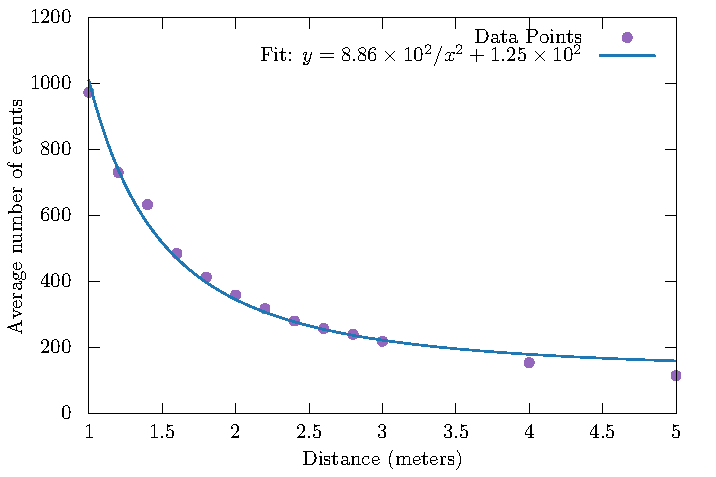
\includegraphics[width=0.90\textwidth]{./fig/semestral/inverse_square/square.pdf}
	\caption{Influence of distance data fitted with various curves.}
	\label{fig:fit1}
\end{figure}
More complex functions could be used to fit the data, but they would likely lead to overfitting rather than capturing the underlying trend in a generalizable way.
The inverse square law provides a relatively good approximation of the data.

\subsection{Rotation angle influence}
From the manufacturers datasheet for the UV LEDs\footnote{The datasheet of ProLight PM2B-1LLE 1W UV Power LED can be obtained from \url{https://www.tme.eu/Document/9dfb498784ffdd07892a42f4f17c6f37/PM2B-1LLE-DTE.pdf}}
used in the UVDAR system, we can learn that the LEDs have a Lambertian radiation pattern,
which can be seen on \reffig{fig:lambertian}.
\begin {figure}[H]
	\centering
	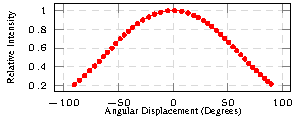
\includegraphics[width=0.75\textwidth]{./fig/semestral/lambertian/lambertian.pdf}
	\caption{Lambertian radiation pattern of the UV LED.}
	\label{fig:lambertian}
\end{figure}

This means that the intensity of the light emitted from the LED decreases with the cosine
of the angle between the normal of the LED and the direction of the light \refeq{eq:lambertian}.
\begin{equation}
	I(\theta) = I_0\cos(\theta)
	\label{eq:lambertian}
\end{equation}
If we shift those distributions by $\pm 45$ degrees and sum them together, we can see the
theoretical distribution of the light emmited from the singular UAV arm \reffig{fig:lambert_combined}.
\begin {figure}[H]
	\centering
	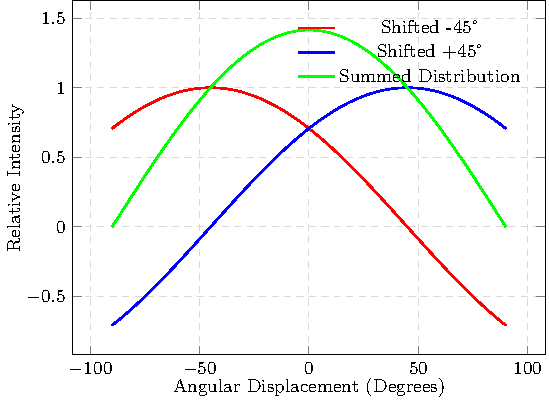
\includegraphics[width=0.50\textwidth]{./fig/semestral/lambertian/3lambertian.pdf}
	\caption{Radiation pattern of two lambertian light sources shifted by $\pm 45$ degrees.}
	\label{fig:lambert_combined}
\end{figure}
With the dataset of the rotation of the UAV relative to the camera we will get the following results
on \reffig{fig:angles}.

\begin{figure}[H]
	\centering
	\subfloat[Influence of rotation of the UAV on the log of average number of events at 0.5 m.] {
	  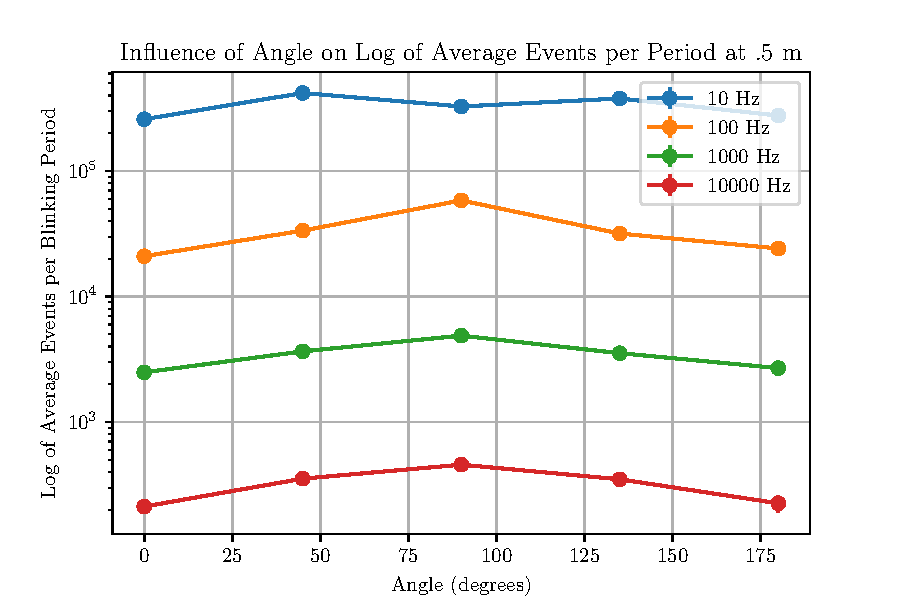
\includegraphics[width=0.5\textwidth]{./fig/semestral/angle1.pdf}
	  \label{fig:angle_1}
	}
	% \subfloat[Influence of rotation of the UAV on the log of average number of events at 1 m.] {
	%   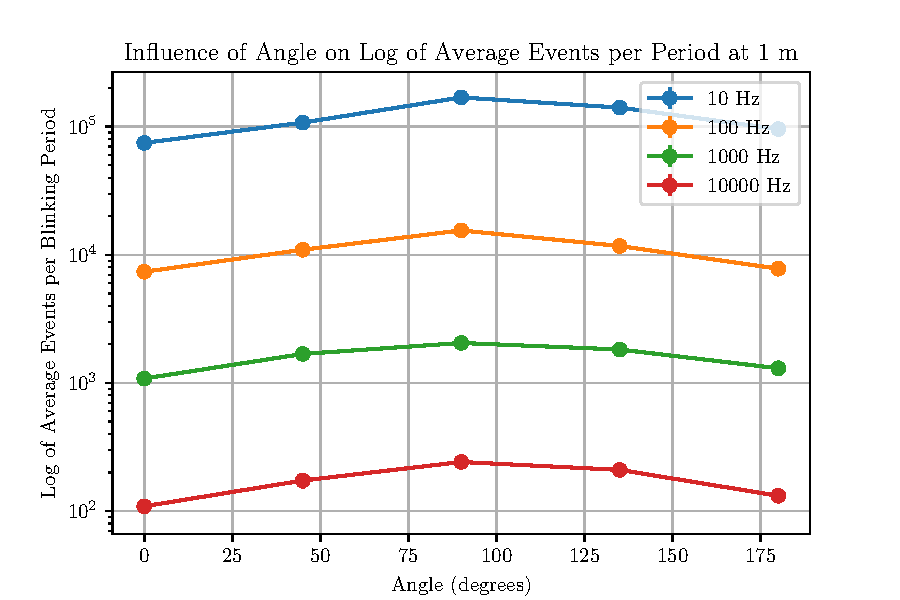
\includegraphics[width=0.5\textwidth]{./fig/semestral/angle2.pdf}
	%   \label{fig:angle_2}
	% }
	\subfloat[Influence of rotation of the UAV on the log of average number of events at 2 m.] {
	  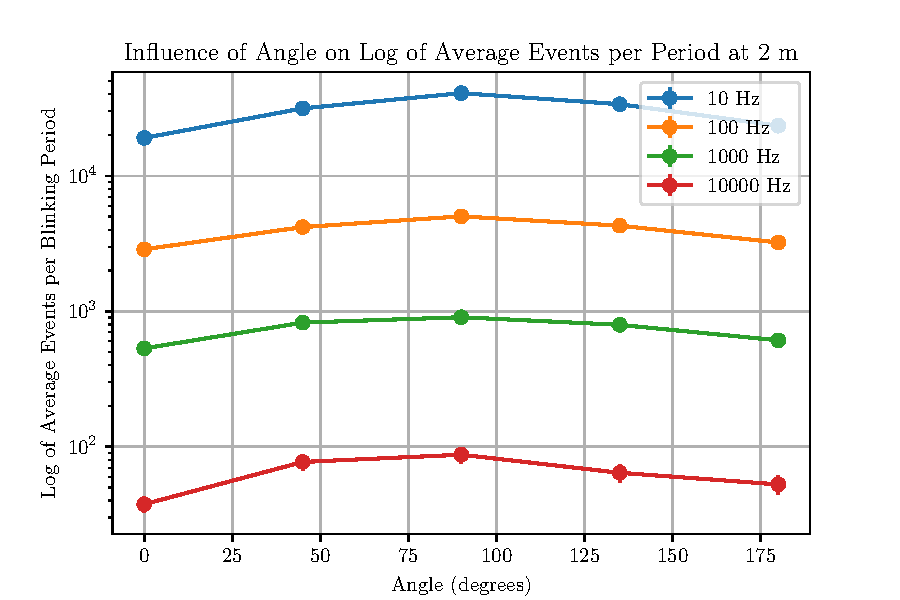
\includegraphics[width=0.5\textwidth]{./fig/semestral/angle3.pdf}
	  \label{fig:angle_3}
	}
	\caption{
  The influence of rotation angle on the log of average number of events at 0.5 m on \reffig{fig:angle_1} and at 2 m on \reffig{fig:angle_3}.
  }
	\label{fig:angles}
\end{figure}
The data show a rough approximation of the theoretical distribution on \reffig{fig:lambert_combined},
but with a drop of intensity at the middle of the distribution. This could be caused
by the fact that LEDs, when close to the camera, can be perceived as multiple light sources,
but when moved further away, they merge into one source as shown on \reffig{fig:leds}.

\begin{figure}[H]
	\centering
	\subfloat[2 LEDs with blinking frequency of 10 Hz at 0.5 m.] {
	  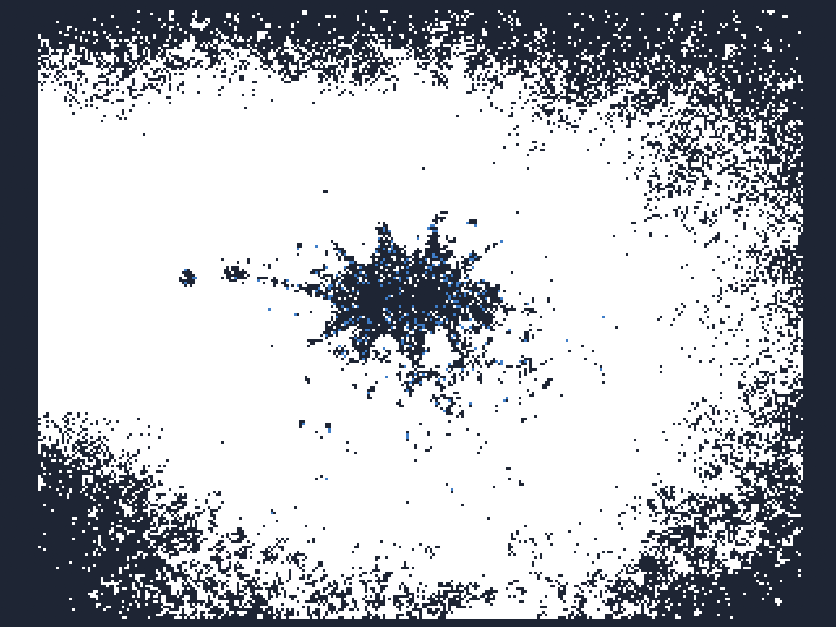
\includegraphics[width=0.5\textwidth]{./fig/photos/2leds_05m.png}
	  \label{fig:leds_1}
	}
	\subfloat[2 LEDs with blinking frequency of 10 Hz at 2 m.] {
	  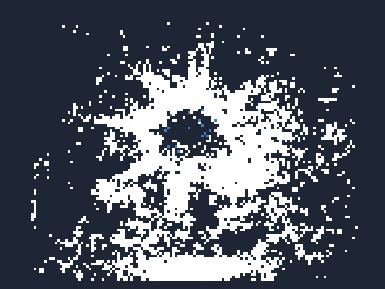
\includegraphics[width=0.5\textwidth]{./fig/photos/2leds_2m.png}
	  \label{fig:leds_2}
	}
	\caption{
  The light source on one arm of the UAV, consisting of two UV LEDs, blinking at a frequency of 10 Hz,
  placed at 0.5 m on \reffig{fig:leds_1} and 2 m at \reffig{fig:leds_2}.
  }
	\label{fig:leds}
\end{figure}
What we can also observe from \reffig{fig:leds} are the star-like shapes of the LEDs, which are supposed to be circular.
Those shapes are caused by light diffraction (and are named diffraction spikes), which are, in turn, caused by the aperture
blades in the lens of the camera. The number
of star spikes depend on the number of blades, the set aperture and the light source intensity then causes stars of different
levels of profoundness.\cite{lendermann2018computational} We can observe this by comparing how profound the star shapes are on different
frequencies, as shown on \reffig{fig:stars}.

\begin{figure}[H]
	\centering
	\subfloat[LED blinking at 10 Hz at 1.0 m] {
	  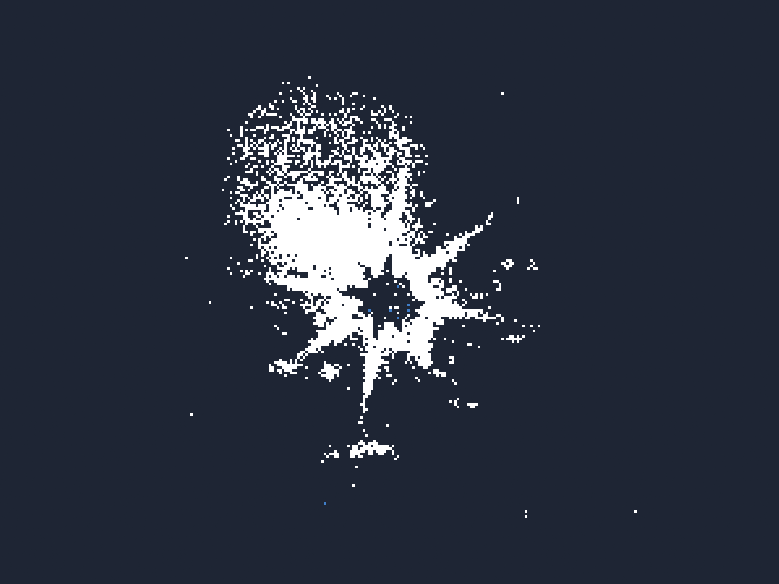
\includegraphics[width=0.5\textwidth]{./fig/photos/led_10hz.png}
	  \label{fig:stars_1}
	}
	\subfloat[LED blinking at 1 kHz at 1.0 m] {
	  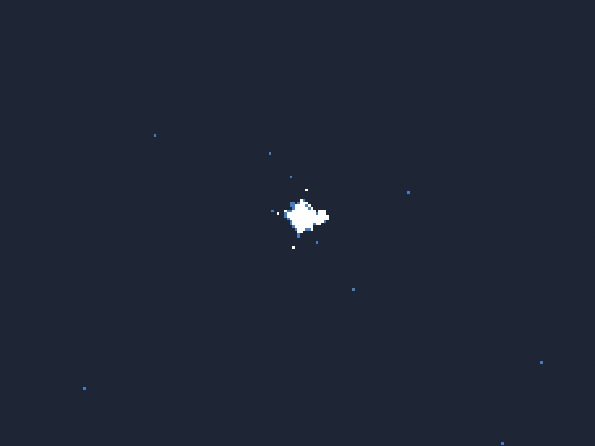
\includegraphics[width=0.5\textwidth]{./fig/photos/led_1000hz.png}
	  \label{fig:stars_2}
	}
	\caption{
  Two same LED light sources at 1.0 meters, blinking at 10 Hz and 1 kHz.
  \reffig{fig:stars_1} shows a visible diffraction star (while being much brighter), while \reffig{fig:stars_2} shows a
  much more cicular source of light that is not as bright.
  }
	\label{fig:stars}
\end{figure}

%% --------------------------------------------------------------
%% |                   Relative pose estimation                 |
%% --------------------------------------------------------------

%!TEX root = ../main.tex

\chapter{Camera calibration\label{chap:calib}}

\section{Method used}

For the correct representation of distances and angles in the received data from the camera, a camera calibration needs to be performed.
The lens used to obtain the data is a 2.5mm f / 1.6 fisheye lens, with a FOV of more than 90 degrees, which can be seen in \reffig{fig:fisheye_lens}.
\begin{figure}[H]
  \centering
  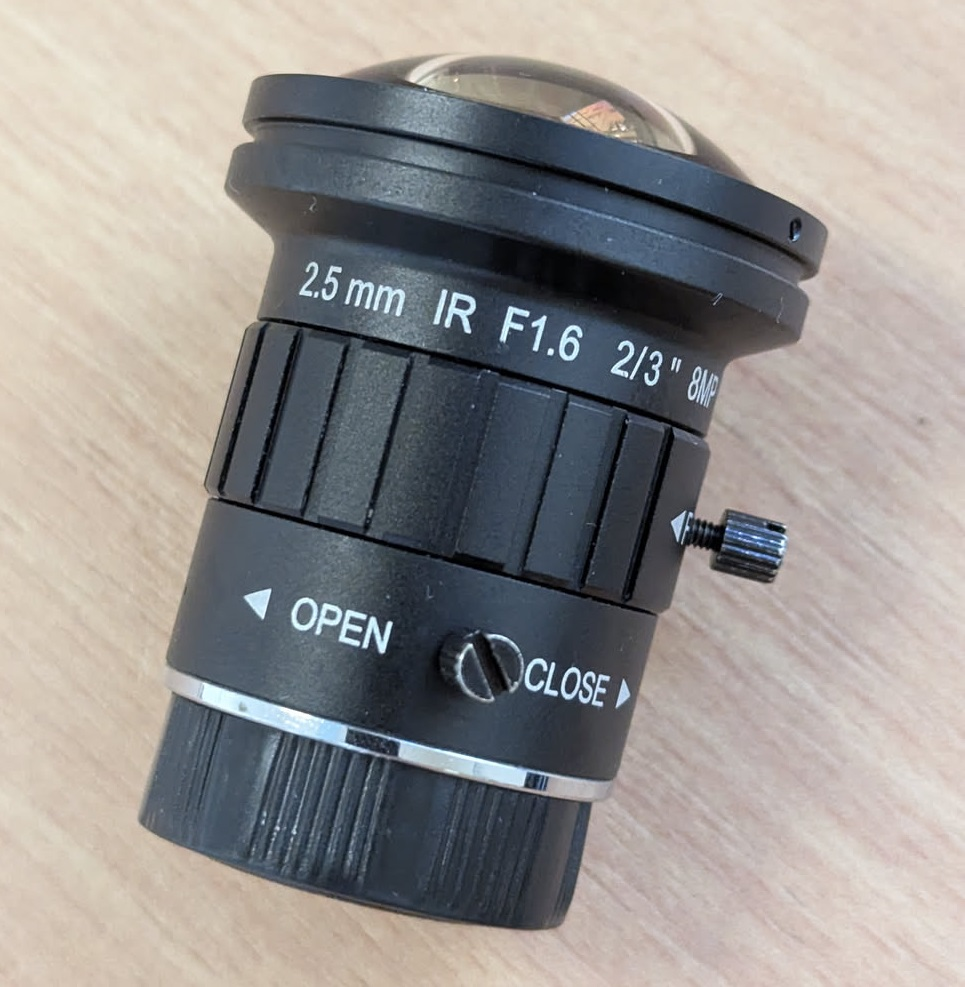
\includegraphics[width=0.5\textwidth]{./fig/photos/lens.jpeg}
  \caption{2.5mm f/1.6 fish eye lens.}
  \label{fig:fisheye_lens}
\end{figure}
In this work a calibration method proposed by Scaramuzza et al. \cite{scaramuzzacalibration} is used, which is based on the pinhole camera model, and is
used to calibrate fish eye lenses. The implementation used for calibration is a Python library py-OCamCalib \footnote{py-OCamCalib is available at \url{https://github.com/jakarto3d/py-OCamCalib}}.%TODO: maybe cite the github repo
For calibration purposes, a calibration chessboard pattern is usually used, which offers high contrast between squares (and thus easy detections of square corners) and
a known square size. Multiple images are usually taken, at various rotations and distances, to obtain good calibration results.
In our calibration procedure, we use a 5x7 lattice of UV LEDs, which are spaced 50 mm apart from each other. With this pattern, events are generated at the center of the
LEDs and can be detected by any kind of blob detector. The LED lattice is used, so the event camera can easily detect events from bright LEDs, as opposed to
the light being reflected from the chessboard pattern (which does not produce any light on its own).
The calibration lattice can be seen in \reffig{fig:lattice}.

\begin{figure}[H]
	\centering
	\subfloat[Calibration lattice] {
	  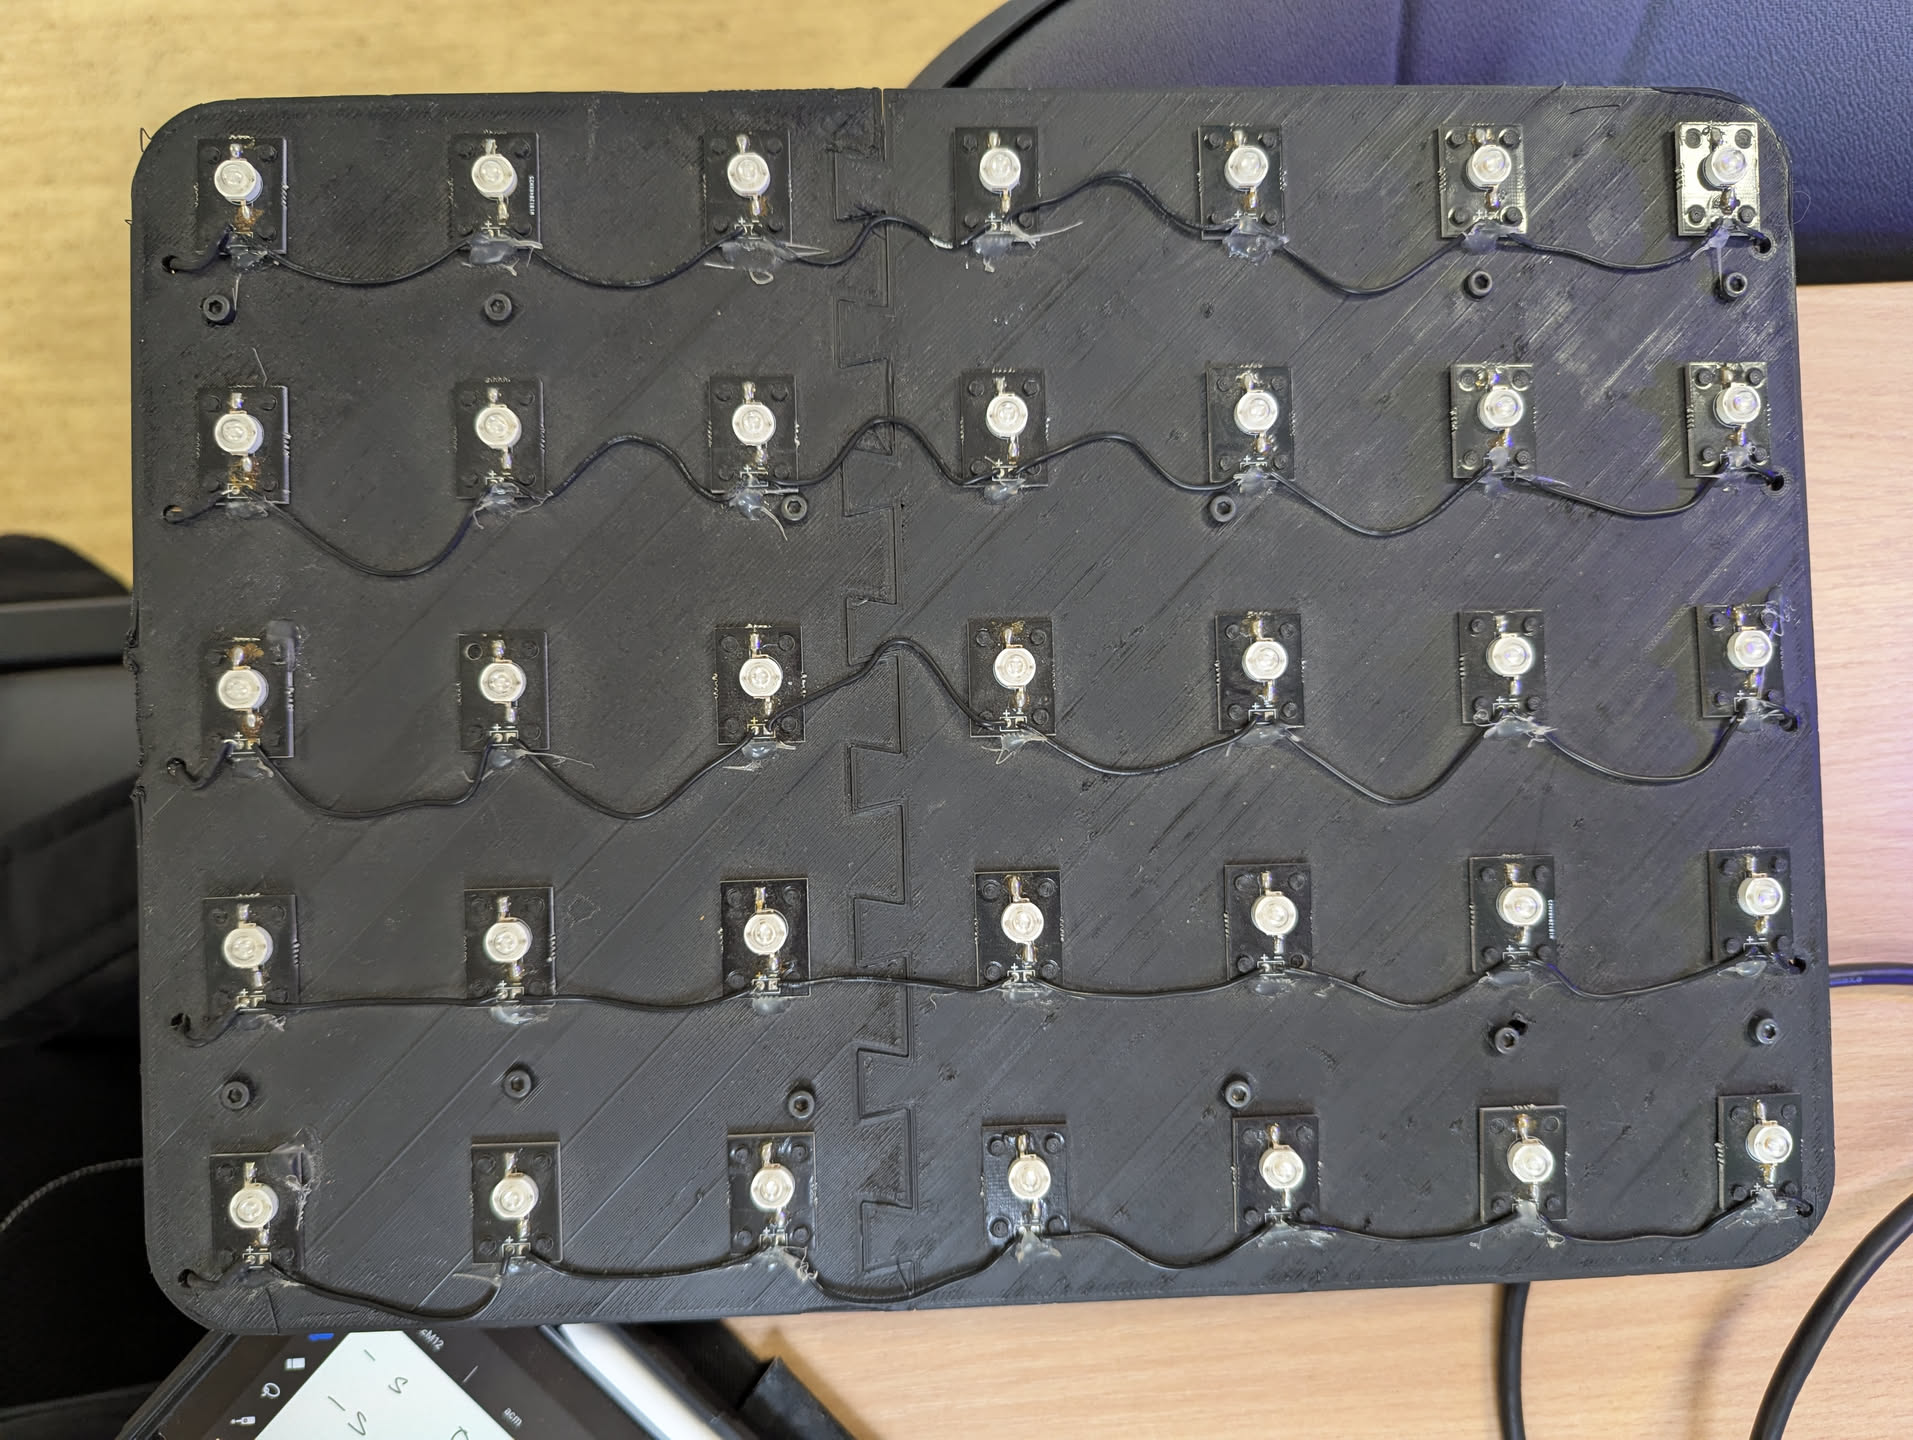
\includegraphics[width=0.5\textwidth]{./fig/photos/lattice.jpeg}
	  \label{fig:lattice_1}
	}
	\subfloat[Image from the event camera of the calibration lattice] {
	  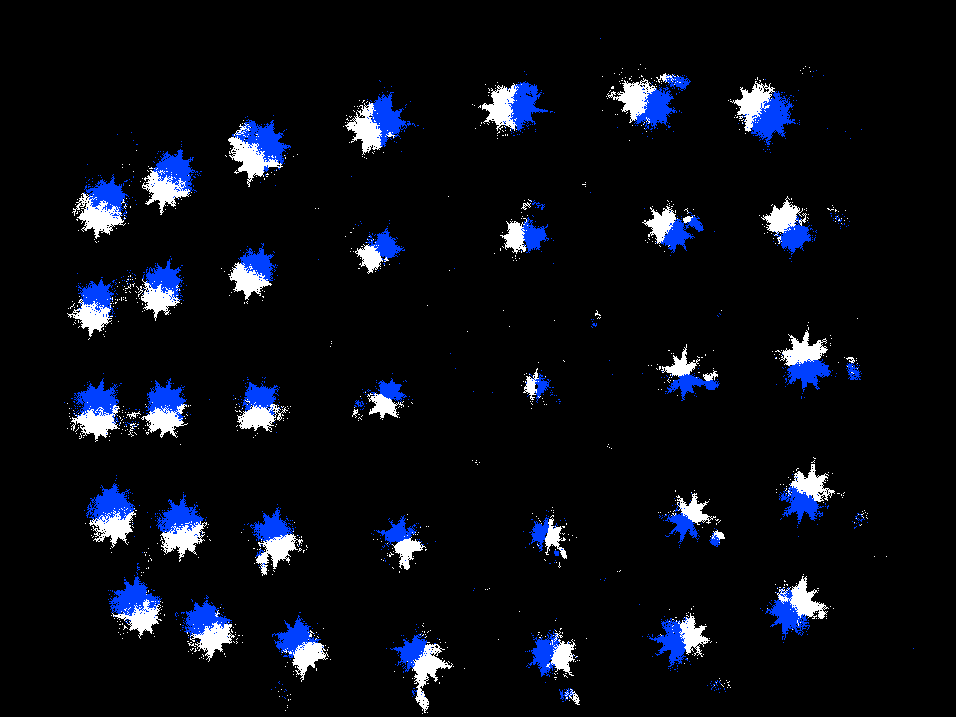
\includegraphics[width=0.5\textwidth]{./fig/photos/lattice_evs.png}
	  \label{fig:lattice_2}
	}
	\caption{
		Calibration lattice of 5x7 UV LEDs on \reffig{fig:lattice_1} and the events being produced when placed in front of the camera at \reffig{fig:lattice_2},
		with typical fish-eye lens distortion.
  }
	\label{fig:lattice}
\end{figure}
The downside of using an LED lattice instead of a chessboard pattern is that at a very high FOV, the distortion of the fish eye lens sometimes does not allow
reliable detection of the exact blob centers (or which events correspond to which LED), as can be seen at \reffig{fig:calibration_pattern_distorted}.
\begin{figure}[H]
  \centering
  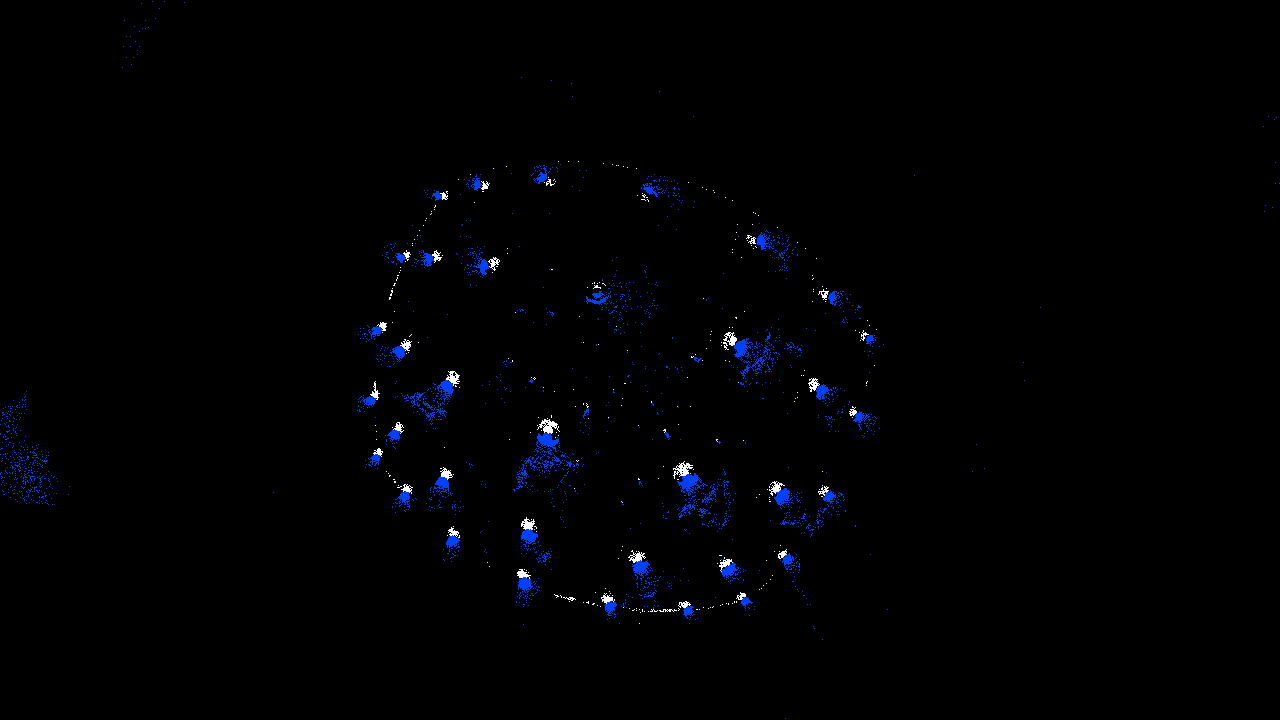
\includegraphics[width=0.7\textwidth]{./fig/photos/lattice_280.png}
  \caption{Calibration pattern with 5x7 lattice of UV LEDs, taken with a lens with FOV of 280 degrees.}
  \label{fig:calibration_pattern_distorted}
\end{figure}

As we are not using a regular image of a chessboard pattern, rather a recording of accumulated events, some data preprocessing has to be done beforehand.
For the purpose of this, a simple Python app has been written. An event raw recording is loaded, and events are accumulated over a select period of time.
The accumulated events are then saved to a grayscale image, where each pixel corresponds to the number of events that occurred in that
pixel \footnote{\url{https://github.com/kubakubakuba/metavision-pyocamcalib/blob/main/generate_frames.py}}. The image is then normalized,
and the LED centers are detected using the \texttt{findContours} function of OpenCV \footnote{\url{https://github.com/kubakubakuba/metavision-pyocamcalib/blob/main/detect_blob_centers.py}}.
The detected centers can then be manually labeled (with optional corrections) row-wise, so the calibration script can then perform the calibration.
After this, the regular calibration script from py-OCamCalib can be used. The labeling of the LED centers can be seen in \reffig{fig:calibration_pattern_labeled}.

\begin{figure}[H]
  \centering
  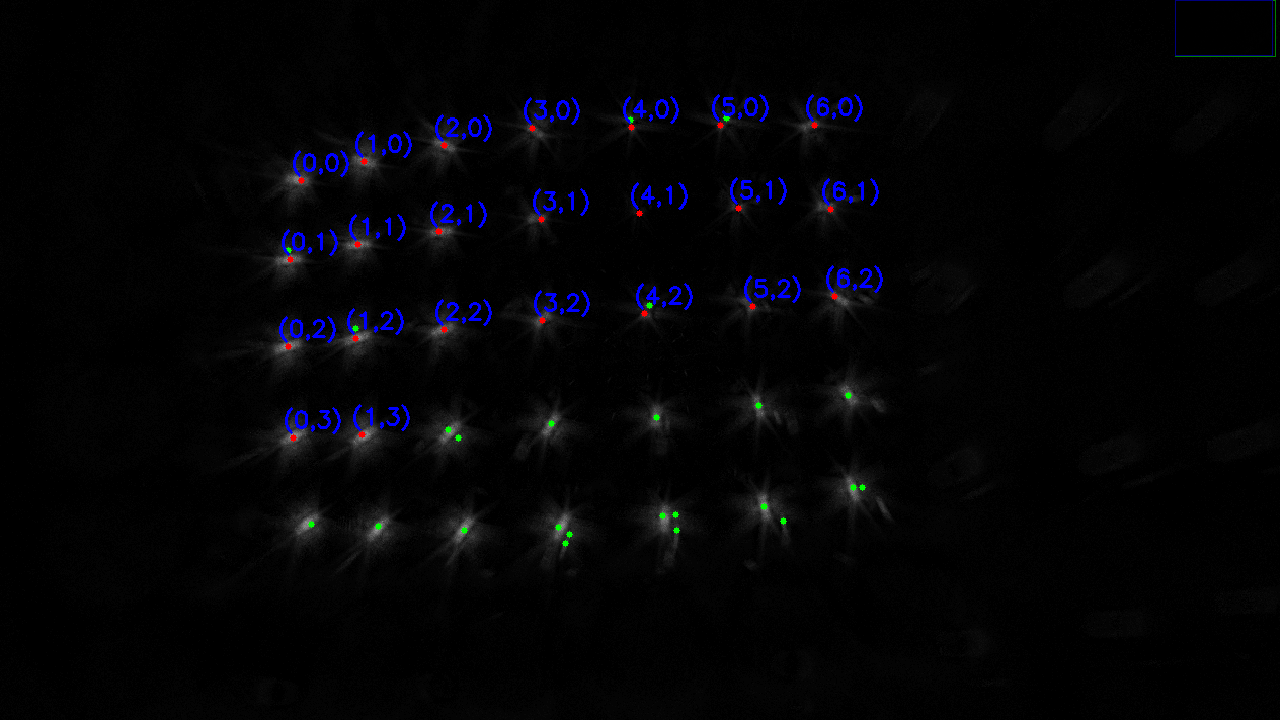
\includegraphics[width=0.7\textwidth]{./fig/photos/lattice_blobs.png}
  \caption{Calibration pattern with 5x7 lattice of UV LEDs, with the centers of the LEDs being labeled.}
  \label{fig:calibration_pattern_labeled}
\end{figure}

\section{Principles of the calibration}

After the calibration is performed, we are able to map the 3D world coordinates to the 2D image plane. For this, the calibration method needs to obtain the extrinsic
and intrinsic parameters of the camera, where the extrinsic parameters are the rotation and translation of the camera with respect to the world frame and can be expressed by equation \ref{eq:extrinsic},
\begin{equation}
	\begin{bmatrix}
		X_{camera} \\
		Y_{camera} \\
		Z_{camera}
	\end{bmatrix}
	= R 
  \begin{bmatrix}
	X_{world} \\
	Y_{world} \\
	Z_{world}
  \end{bmatrix}
  + T
  \label{eq:extrinsic}
\end{equation}
which is an affine transformation that uses a rotation matrix $R$ and a translation vector $T$. The origin of the camera's coordinate system is at the optical center,
that is, at the intersection of the optical axis from the center of the image with the image plane. This can be represented by \reffig{fig:camera_extrinsic}.

\begin{figure}[H]
  \centering
  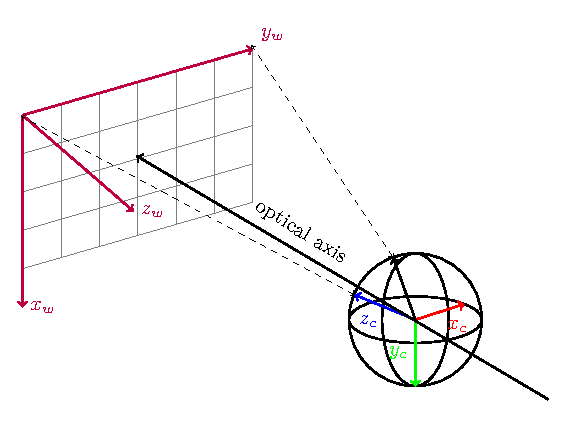
\includegraphics[width=0.7\textwidth]{./fig/tikz/extrinsic.pdf}
  \caption{Extrinsic parameters of the camera.}
  \label{fig:camera_extrinsic}
\end{figure}

The next step in the camera calibration is to fit an encompassing ellipse to the received data. The purpose of this is to see the center of distortion of the fish eye lens, as well
as the stretching of the image on both the x and y axes. This process can be seen in \reffig{fig:ellipse}. This ellipse is then used to calculate the point-mapping functions, which allows for tranformation of points from
the image plane to their respective 3D coordinates.

\begin{figure}[H]
	\centering
	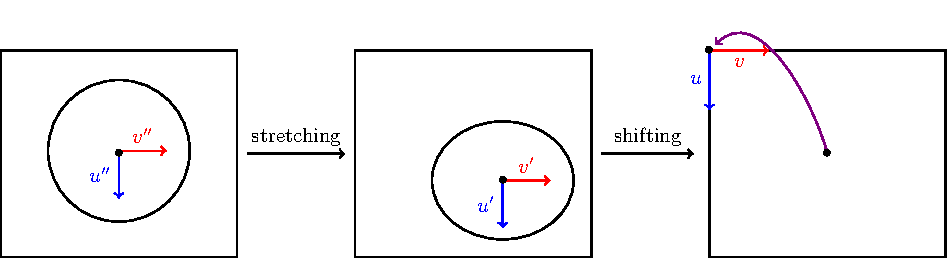
\includegraphics[width=0.9\textwidth]{./fig/tikz/ellipse.pdf}
	\caption{}
	\label{fig:ellipse}
  \end{figure}

The intrinsic parameters of the camera specify the image format itself, which is influenced by the focal length, sensor size, and optical center. As there are many mapping
functions that can be used while modeling the lens (their precision is limited by the manufacturing process), Scaramuzza et al. \cite{scaramuzzacalibration} proposed
fitting a polynomial to find the optimal model for lens calibration. The mapping functions are shown in \reffig{fig:mapping_functions}.
\begin{figure}[H]
  \centering
  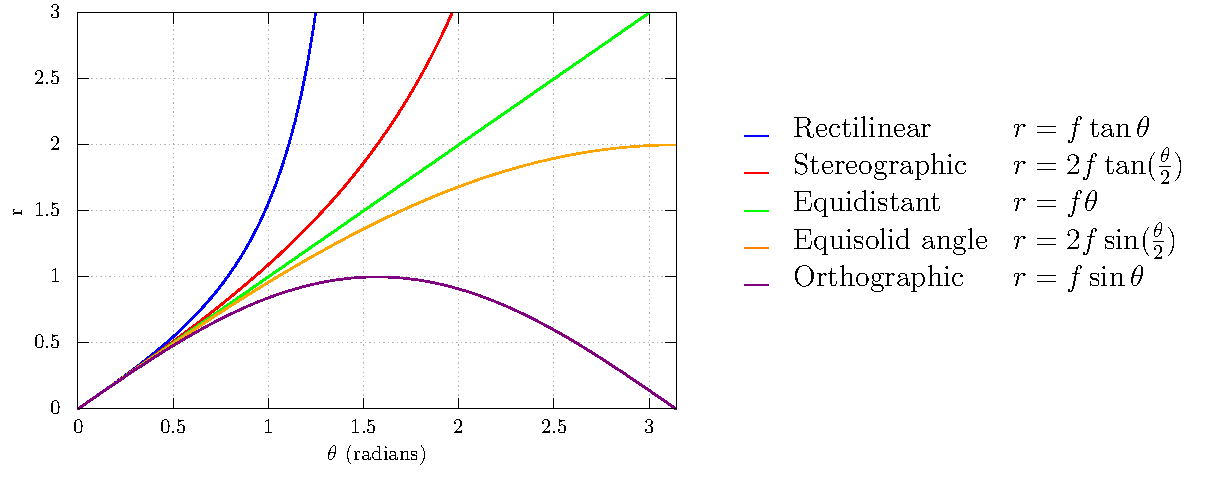
\includegraphics[width=0.9\textwidth]{./fig/tikz/mapping.pdf}
  \caption{Fisheye mapping functions, $f$ is a parameter (focal length).}
  \label{fig:mapping_functions}
\end{figure}

After we fit a polynomial, we can map the image points to their corresponding 3D vectors by an equation \ref{eq:intrinsic}.
\begin{equation}
	\lambda \cdot \alpha \cdot
	\begin{bmatrix}
		u' \\
		v' \\
		a_0 + a_1 \rho + \dots + a_{N} \rho^{N} 
	\end{bmatrix}
	= \mathbf{P} \cdot \mathbf{X_w} = %TODO: DOUBLE CHECK X_w is really the world point 
	\begin{bmatrix}
		X_c \\
		Y_c \\
		Z_c
	\end{bmatrix}
	\label{eq:intrinsic}
\end{equation}
where:

$\lambda$ is a scalar factor

$\alpha$ is a scaling factor that we obtain from \reffig{fig:ellipse} by stretching the ellipse back to a circle and performing
the affine transformation; $\alpha, \lambda > 0$

$\rho$ is the Euclidean distance of a point from the center; $\rho = \sqrt{u^2 + v^2}$

$a_0, \dots a_N$ are the polynomial coefficients and $\mathbf{P}$ is 
the perspective projection matrix.

We can also write another relation between a point $\textbf{m}' = \begin{bmatrix} u' & v' \end{bmatrix}^{T}$ in the image plane
and its corresponding point on the sensor plane $\textbf{m} = \begin{bmatrix} u & v \end{bmatrix}^{T}$. The coordinates of
$\textbf{m}'$ have the origin at the top left corner of the image, whereas the coordinates of $\textbf{m}$ have the origin in the center of the image.
This can be represented by an affine transformation $\textbf{m}' = \textbf{Am} + \textbf{O}_c$, on \ref{eq:affine} \cite{URBAN201572}.

\begin{equation}
	\begin{bmatrix}
		u' \\
		v'
	\end{bmatrix}
	= 
	\begin{bmatrix}
		c & d \\
		e & 1
	\end{bmatrix}
	\begin{bmatrix}
		u \\
		v
	\end{bmatrix}
	+
	\begin{bmatrix}
		o_u \\
		o_v
	\end{bmatrix}
\label{eq:affine}
\end{equation}

where matrix A accounts for lens-sensor misalignment, and the vector $\textbf{O}_c$ captures the relation with the center of the distortion. 

\section{Calibration results}

The camera calibration was performed on a series of images, where the calibration lattice was placed as various angles and distances from the camera.
For ideal calibration results, the lattice should be placed in all visible parts of the image, as the distortion of the fish eye is more pronounced at the edges
of the visible area. The calibration was performed on a polynomial of degree 4, more would lead to overfitting and is also not necessary.
The calibration results can be seen in \reffig{fig:calib_r}.

\begin{figure}[H]
	\centering
	\subfloat[Calibrated lens model function] {
	  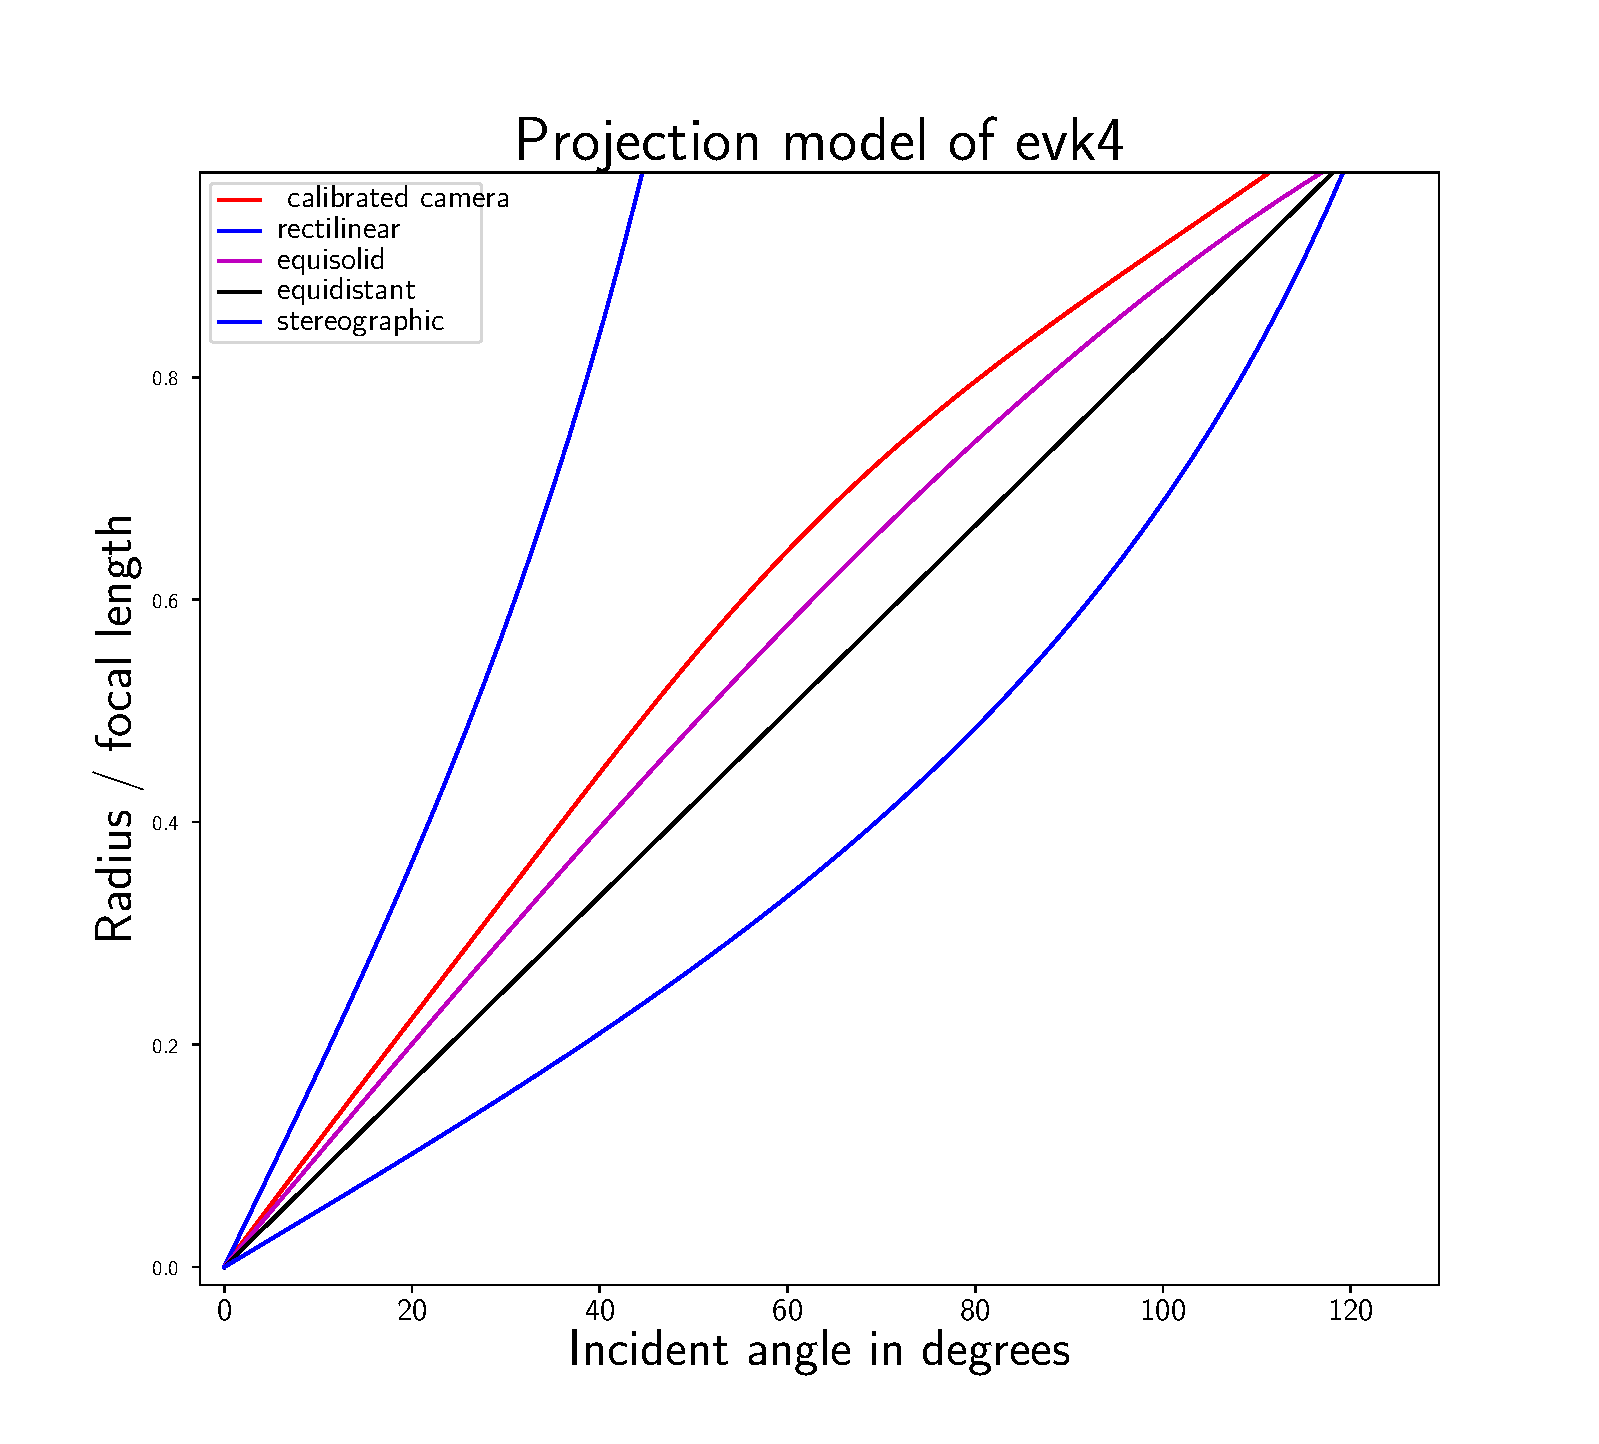
\includegraphics[width=0.5\textwidth]{./fig/pgfplot/evk4_projection.pdf}
	  \label{fig:calib_r_1}
	}
	\subfloat[Calibration images mean reprojection errors] {
	  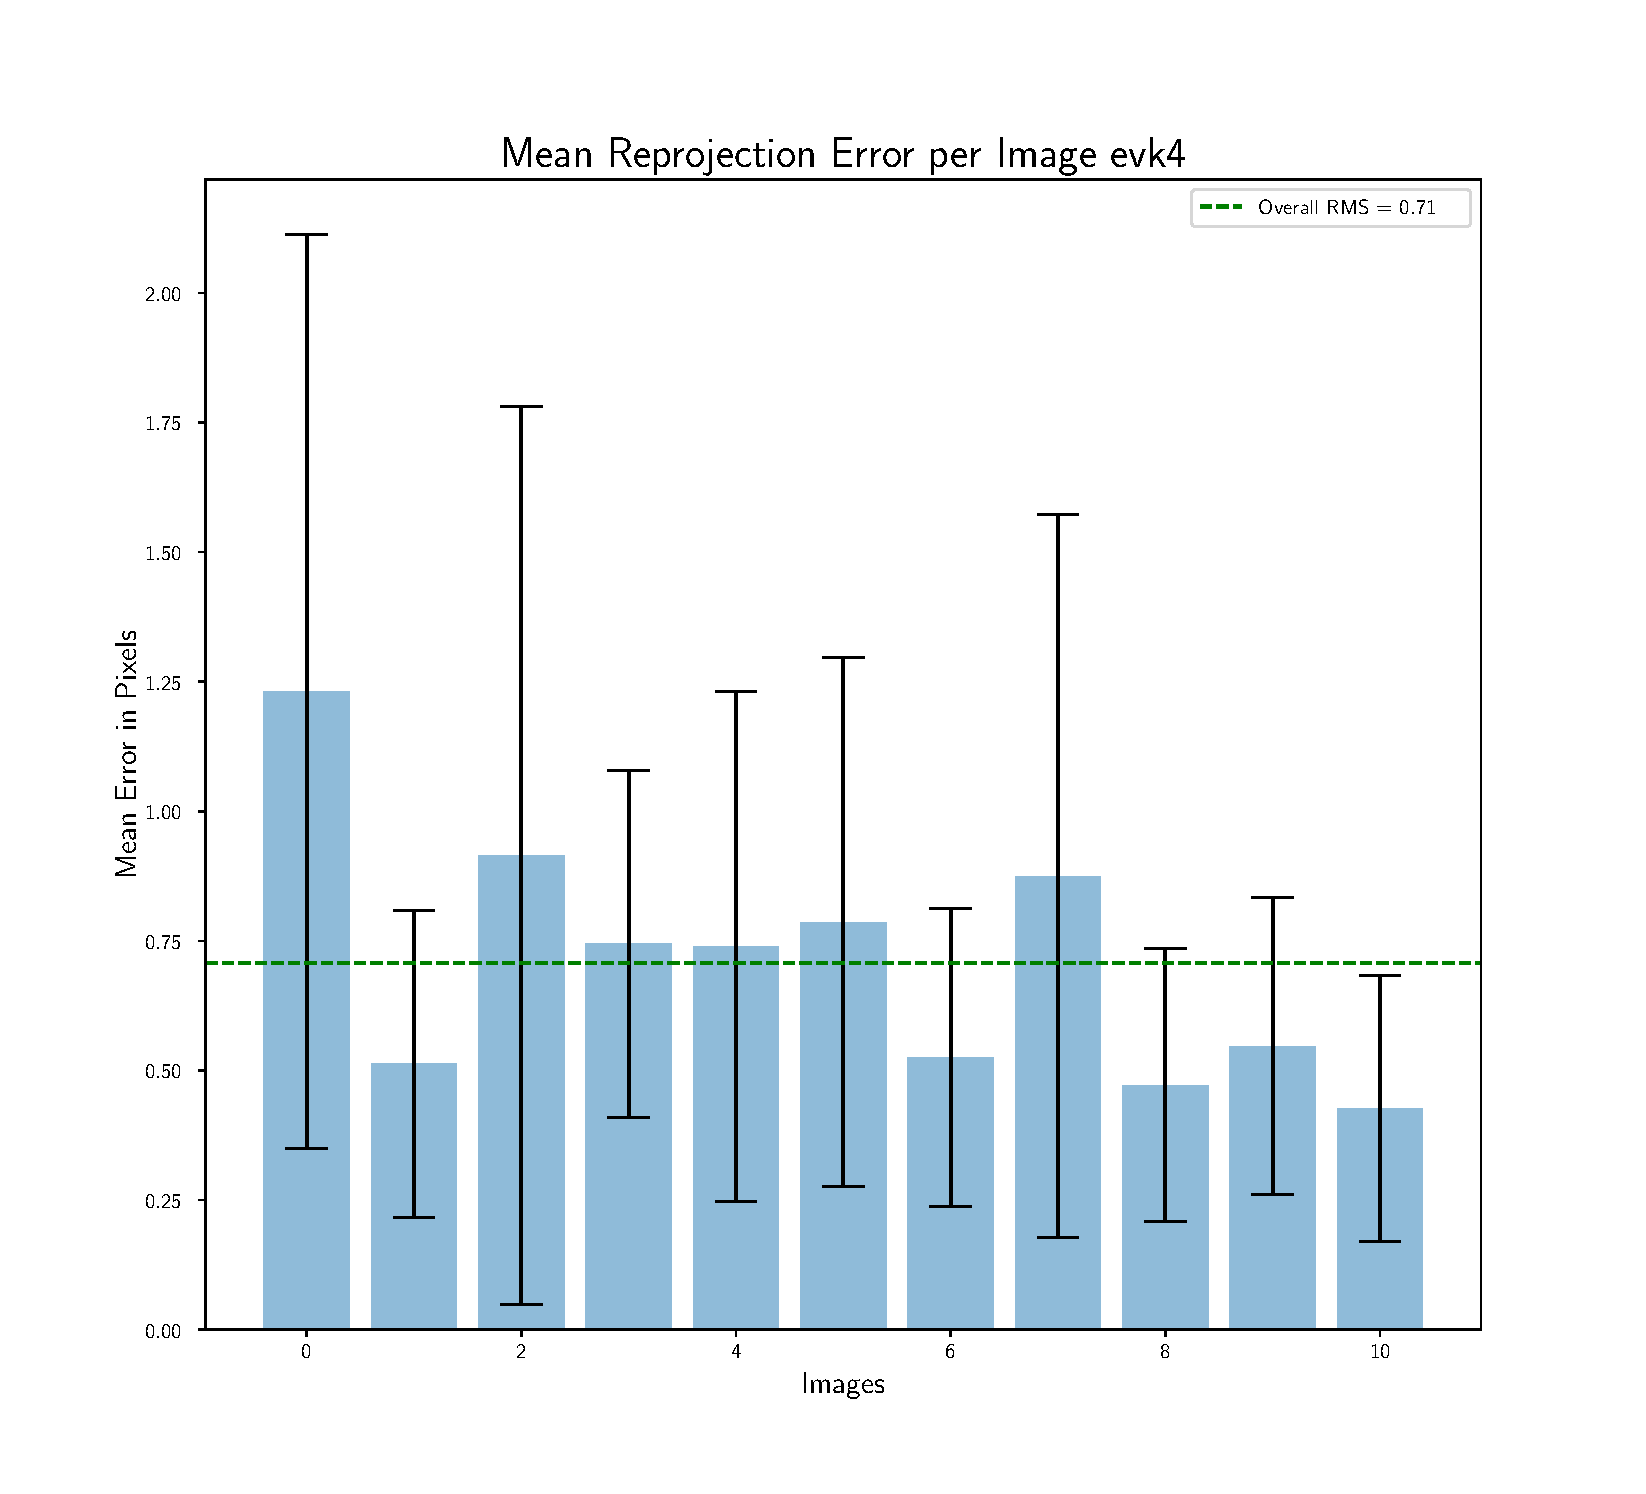
\includegraphics[width=0.5\textwidth]{./fig/pgfplot/evk4_reprojection_error.pdf}
	  \label{fig:calib_r_2}
	}
	\caption{
		Calibration results with the calibrated lens model function highlighted in red in \reffig{fig:calib_r_1} and the calibration images mean reprojection errors on \reffig{fig:calib_r_2}.
  }
	\label{fig:calib_r}
\end{figure}

We can now fit the encompassing ellipse to the data by minimizing the number of events that are outside the ellipse (minimizing the ellipse size while keeping the
captured events inside). The ellipse can be seen in \reffig{fig:ellipse_fit}.
TODO: formulate the optimization problem mathematically
\begin{figure}[H]
	\centering
	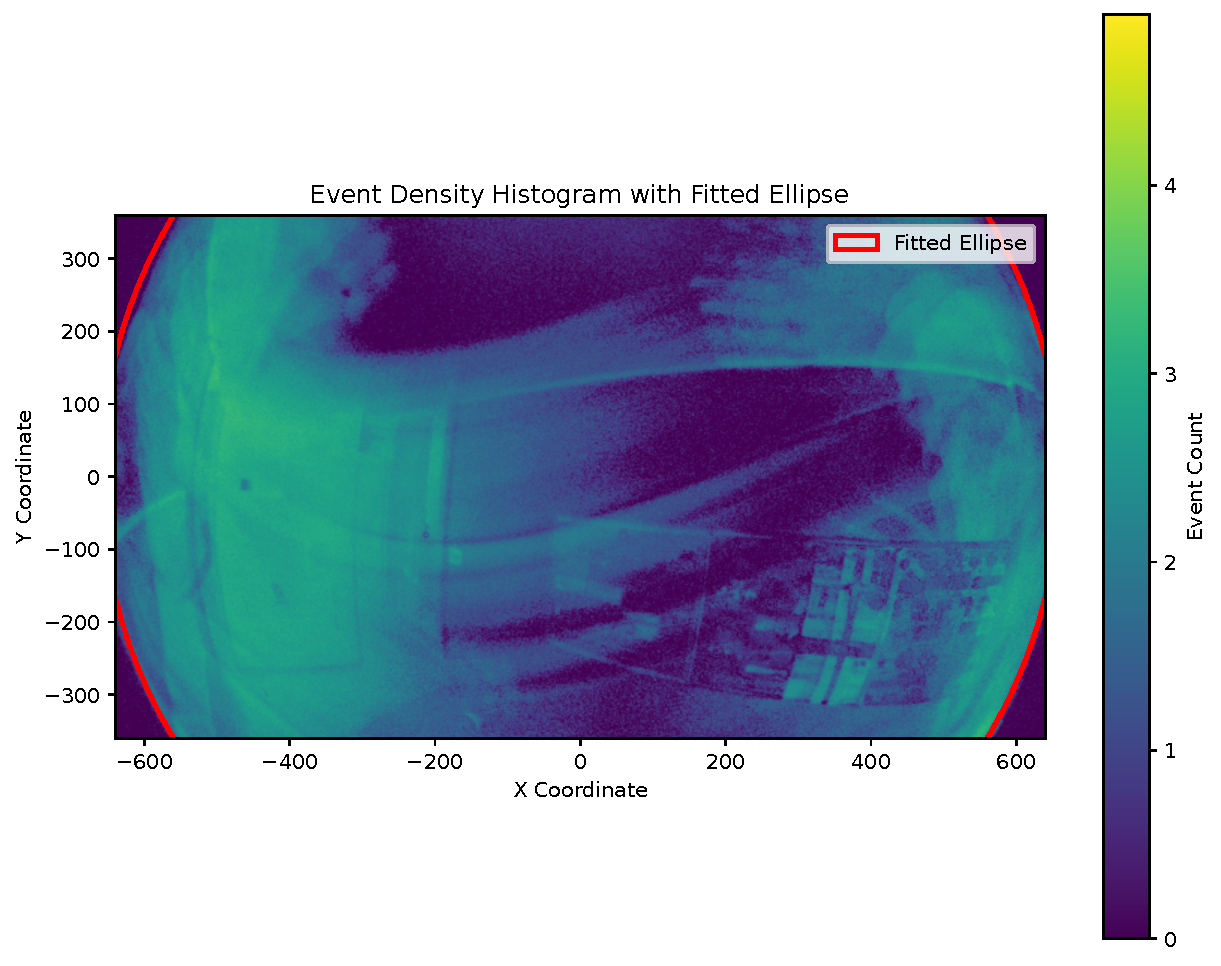
\includegraphics[width=0.7\textwidth]{./fig/svg/ellipse_fit.pdf}
	\caption{Fitted ellipse to the calibration data, with major axis $a = 652$, and minor axis $b = 650$.}
	\label{fig:ellipse_fit}
\end{figure}

Finally, to visualize the calibration results, we map every point from the image plane using the \texttt{cam2world}\footnote{\url{https://github.com/jakarto3d/py-OCamCalib/blob/main/src/pyocamcalib/modelling/camera.py}}
function from py-OCamCalib, which takes a 2D image point, and returns
the corresponding 3D optical ray on the camera's unit sphere. For each point, we calculate its angle from the optical axis (a vector $\mathbf{v} = \begin{bmatrix} 0 & 0 & 1 \end{bmatrix}^{T}$),
and mask out the visible area with the ellipse fitted in \reffig{fig:ellipse_fit}. We can see the results in \reffig{fig:calibration_viz}.

\begin{figure}[H]
	\centering
	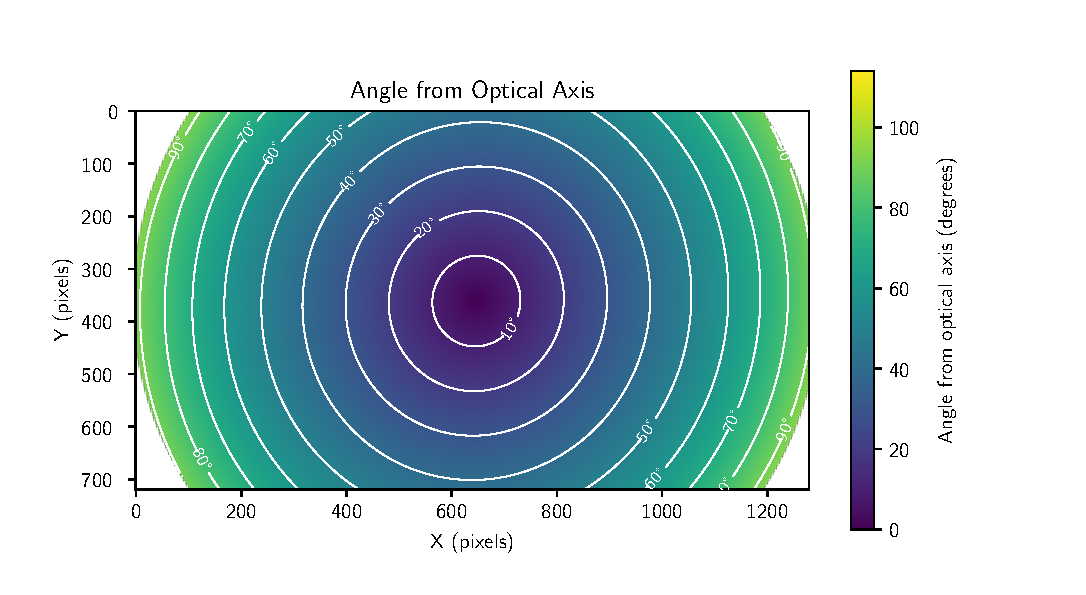
\includegraphics[width=1.0\textwidth]{./fig/pgfplot/evk4_viz.pdf}
	\caption{Angle from optical axis visualization, with the maximum angle of 93.47 degrees.}
	\label{fig:calibration_viz}
\end{figure}

We can also apply a perspective conversion to the whole image, which now correctly represents distances and angles. We can notice this by looking
at the calibration lattice at \reffig{fig:calib_c}, which now looks like a grid of points.

\begin{figure}[H]
	\centering
	\subfloat[Uncalibrated image.] {
	  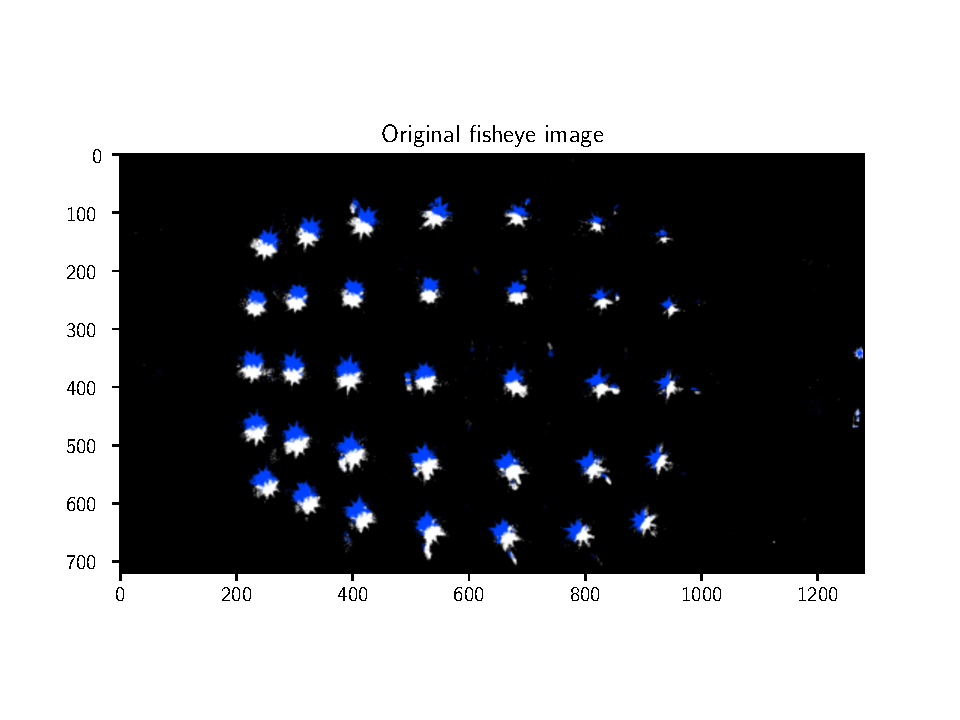
\includegraphics[width=0.5\textwidth]{./fig/pgfplot/image_uncalib.pdf}
	  \label{fig:calib_c_1}
	}
	\subfloat[Calibrated image.] {
	  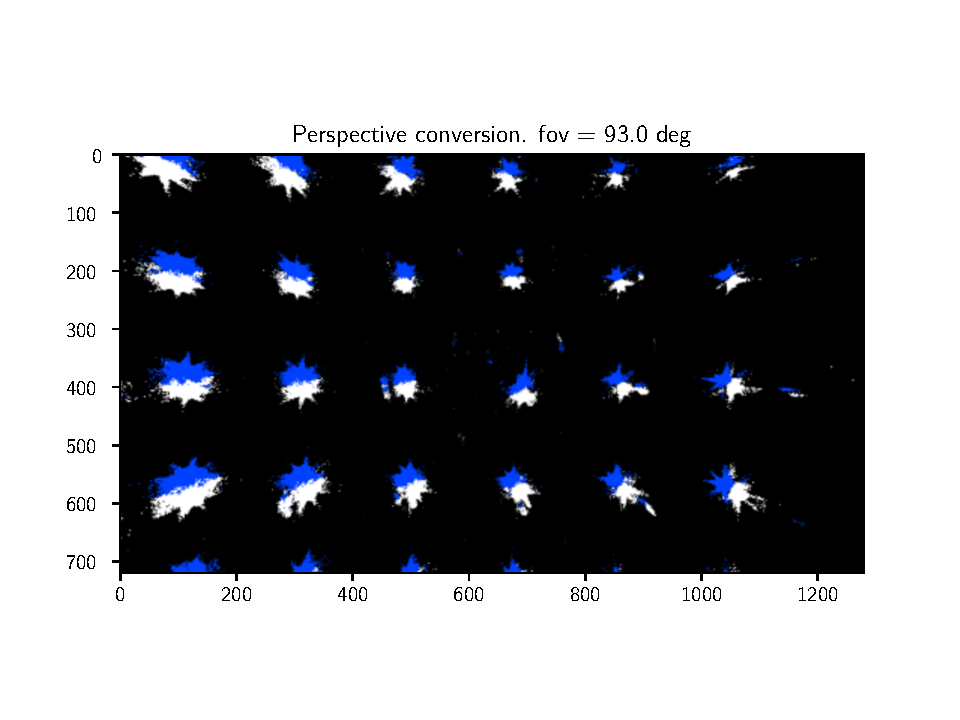
\includegraphics[width=0.5\textwidth]{./fig/pgfplot/image_calib.pdf}
	  \label{fig:calib_c_2}
	}
	\caption{
		Two photos of the calibration lattice, one uncalibrated on \reffig{fig:calib_c_1} and the one calibrated at \reffig{fig:calib_c_2}, which does not
		exhibit any distortion.
  }
	\label{fig:calib_c}
\end{figure}

%% --------------------------------------------------------------
%% |                    Distance estimation                     |
%% --------------------------------------------------------------

%!TEX root = ../main.tex

\chapter{Distance estimation\label{chap:p3p}}

For distance estimation, one can leverage many different approaches, either directly relying on the event data stream itself, or integrating the
events over time (thus producing a grayscale image or a heatmap), and then estimating the position from the produced image. As we have shown in \refchap{chap:response}, the number of events
generated by \ac{LED} sources decreases monotonically with the square of the distance and also decreases with increasing modulation frequency.
We could then assume that a simple distance predictor could be made by simply fitting a curve to the training dataset consisting of an average
number of events per blinking period (thus training this predictor for average number of events with respect to distance) and then making the prediction of distance by calculating the average in real time and getting an estimation from the trained predictor.

This is possible to do in very specific cases where the camera settings and the scene lighting conditions do not change between training measurements
and the deployment. For example, changing the \texttt{bias-diff-on} or \texttt{bias-diff-off} settings of the camera changes the brightness-change threshold on
which the camera generates events.
This changes the number of events that are generated without any information on the distance from the camera, this is similar to changing the exposure
time on a global shutter camera, which can then give an under- or over-exposed frame.
It also does not generalize the problem of estimating the position of an arbitrary \ac{UAV} marked with \ac{LED} lights and a camera with previously unspecified
settings. For a more robust way of estimating the pose of the \ac{UAV} from the camera, we can leverage the following methods.

\section{RSSR}

The \ac{RSSR} method provides an approach to estimate the position of an object by measuring the relative ratio of received optical powers from \ac{LED}
markers. This is done by making each of the \ac{LED} markers radiate in their assigned time slot, measuring their optical powers at the time of the
radiation. Jung et al. (2014) \cite{sooyongrssr} demonstrated the \ac{RSSR} method using a configuration where four LED lamps were mounted on the ceiling
with a detector mounted on top of a moving object, parallel to the ceiling.
They have arrived at the equation \refeq{eq:rssr} which could be used to describe the power ratio $RSSR_{1,2}$
\begin{equation}
RSSR_{1,2} = \frac{P_{R1}}{P_{R2}} = \left( \frac{d_2}{d_1} \right)^{n+3}
\label{eq:rssr}
\end{equation}
where $P_{R1}$ and $P_{R2}$ are the received powers of the \ac{LED}s, $d_1$ and $d_2$ are the distances to the \ac{LED}s, and $n$ is the mode number of the radiation lobe (for a Lambertian model $n = 1$).

\section{Perspective-n-Point}
The \ac{PnP} problem addresses the estimation of the position of an object relative to the camera, having six \ac{DOF}
\begin{itemize}
\item{Rotation - roll, pitch and yaw}
\item{Translation - 3D vector representing the position of the object relative to the camera}
\end{itemize}
This estimation is performed given a set of $n$ known 3D points $\{\mathbf{P}_i\}_{i=1}^n$ on the object and their corresponding 2D projections $\{\mathbf{p}_i\}_{i=1}^n$ in the image plane.
In our application, the UAV has four \ac{LED}-marked arms, where each of them is distinguishable by the camera as a point light source.
However, due to physical limitations, only three \ac{LED}s may be visible at a single point in time, the fourth obstructed by the physical structure of the \ac{UAV} when viewed from the front.
For a case of only 3 image points, the problem becomes the minimal solvable case, called \ac{P3P}, which 
can be formulated as a set of 3D points $\textbf{P}_i \in \mathbb{R}^{3}, i \in \{1, 2, 3\}$ in the world coordinate system, with their corresponding normalized image points
$\textbf{p}_i \in \mathbb{R}^{2}$, $|\textbf{p}_i|=1, i \in \{1, 2, 3\}$. These sets of points are related by a rigid transformation \cite{Ding_2023_CVPR}
\begin{equation}
d_i \textbf{p}_i = \textbf{R} \textbf{P}_i + \textbf{t}
\label{eq:p3p}
\end{equation}
where $d_i \in \mathbb{R}^+$.
Given the rigid transformation relationship shown in \refeq{eq:p3p}, the \ac{P3P} problem reduces to solving for the rotation matrix 
$\mathbf{R} \in \text{SO}(3)$, translation vector $\mathbf{t} \in \mathbb{R}^3$, and depths $d_i > 0$. 
By exploiting geometric constraints between the 3D points and their 2D projections, the problem can be
reformulated algebraically and solved using various techniques. In our approach, we use the method proposed by Kneip et al. \cite{kneip}, which
directly finds the rotation and translation with a novel parameterization of the model.
The visualization of the \ac{P3P} problem is shown on \reffig{fig:p3p}.
\begin{figure}[H]
	\centering
	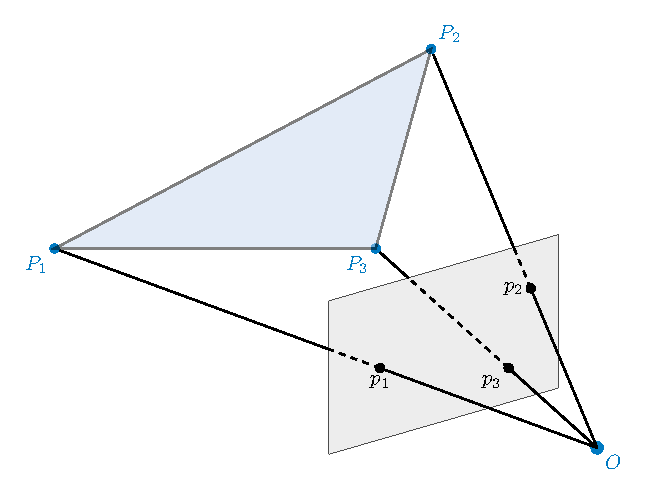
\includegraphics[width=0.65\textwidth]{./fig/tikz/p3p.pdf}
	\caption{P3P problem visualization}
	\label{fig:p3p}
\end{figure}
In our implementation, we compute the average of the estimated pose and distance, thus simplifying the problem of identifying the correct solution. If all four \ac{LED}s on the \ac{UAV} are detected, a general \ac{PnP} solution is calculated using the \ac{RANSAC} method. This yields only one solution, so the
estimated distance is simply the distance from the camera to the geometrical center of the \ac{UAV}.

\section{Stationary experiment\label{sec:stationary_experiment}}
An experiment with a stationary \ac{UAV} and event-based camera was conducted prior to the experiment with flying \ac{UAV}s to ensure functionality.
A \ac{UAV} was placed at the floor several meters from the camera and rotated around to obstruct one \ac{LED} in some measurements to test out \ac{P3P}. The \ac{LED} blinking frequencies were set to $\mathcal{F} = \{125, 250, 500, 1000\}$ Hz, and a blob detector was used to detect the centers of the visible blobs. The individual \ac{LED}s were identified by their visible
brightness differences (which were influenced by the event-based camera response to the blinking frequencies) and by the known physical structure of the \ac{UAV}. The view from the event-based camera can be seen on \reffig{fig:pnpuav}.
\begin{figure}[H]
	\centering
	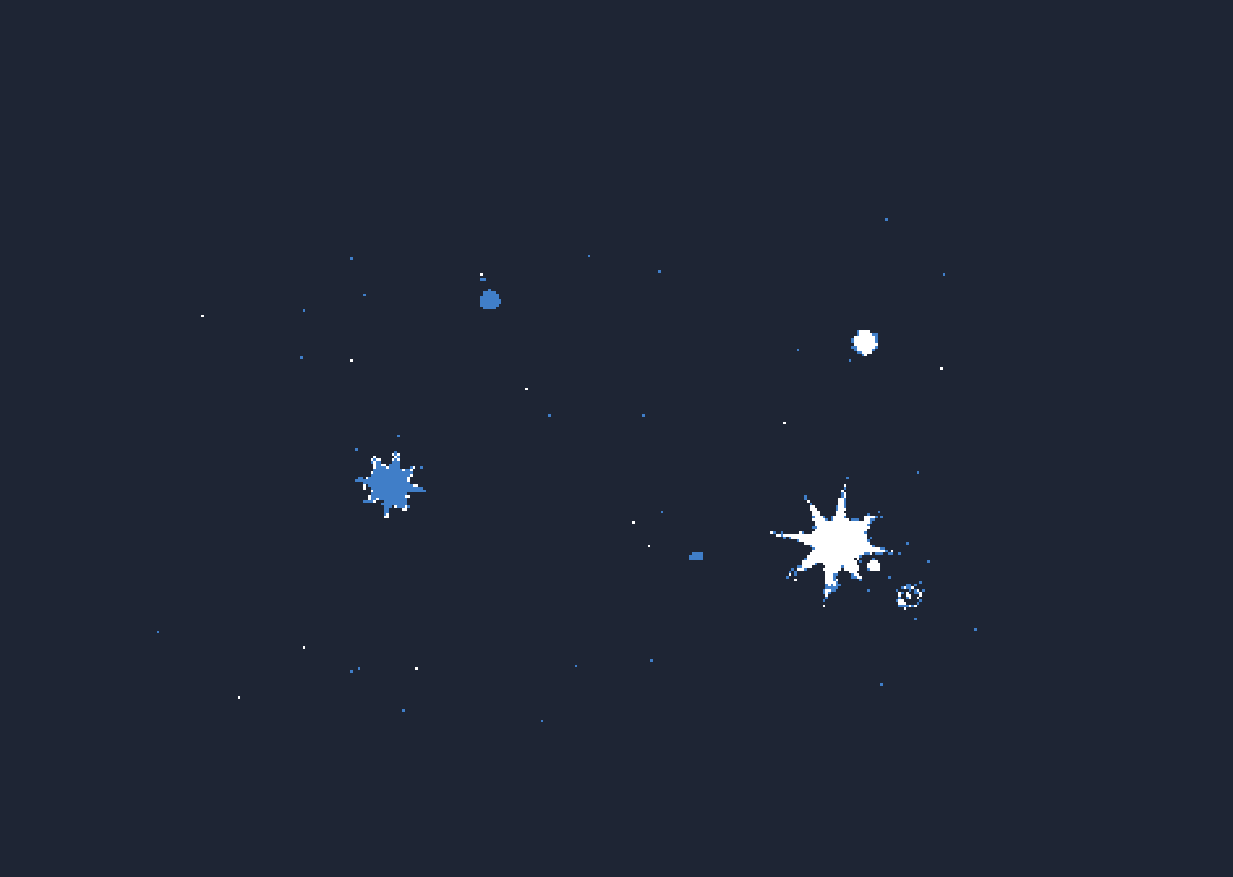
\includegraphics[width=0.65\textwidth]{./fig/photos/pnpmeas.png}
	\caption{Data from the stationary experiment}
	\label{fig:pnpuav}
\end{figure}
Then a \ac{PnP} (\ac{P3P}) estimation was performed with a calibrated camera, the ground truth data being the measured distance from the camera to the
stationary \ac{UAV} placed on the ground.
The results can be seen on \reffig{fig:pnpres}, with several recordings
present for each distance. The mean distance estimation error was $0.34$ meters with a standard deviation of $0.16$ meters.
\begin{figure}[H]
	\centering
	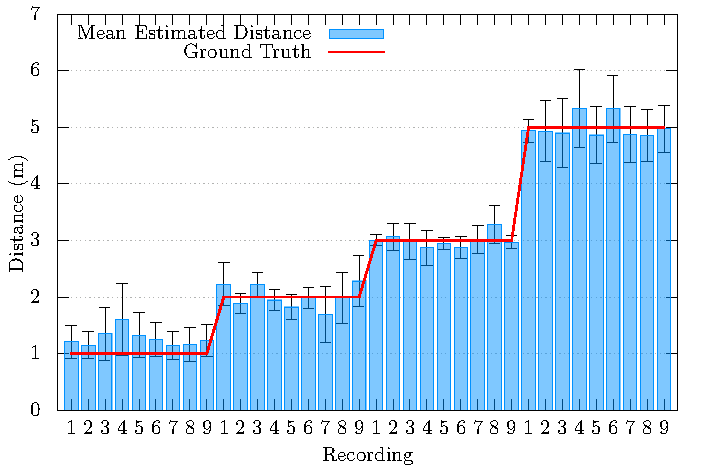
\includegraphics[width=0.75\textwidth]{./fig/tikz/pnp_results.pdf}
	\caption{PnP estimation results}
	\label{fig:pnpres}
\end{figure}

\section{ROS implementation}
To facilitate the deployment on real hardware, a \ac{ROS} \texttt{DistanceEstimator} node was implemented
\footnote{The source code of the distance estimator \ac{ROS} node is available at \url{https://github.com/kubakubakuba/ros-event-distance}}.
The functionality can be summarized with the flow chart
in
\reffig{fig:rosflow}.
\begin{figure}[H]
	\centering
	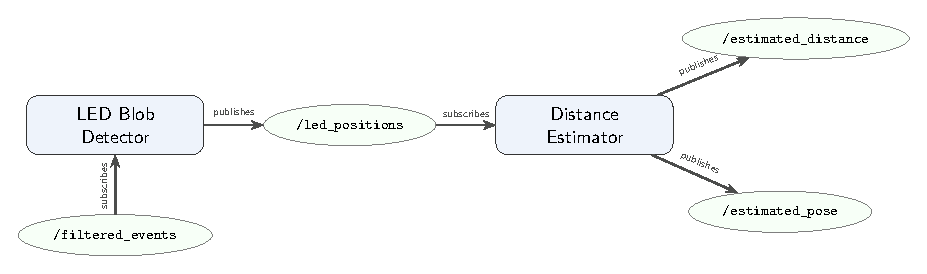
\includegraphics[width=1.0\textwidth]{./fig/tikz/rosflow.pdf}
	\caption{ROS distance estimation pipeline}
	\label{fig:rosflow}
\end{figure}
On the input, a filtered event stream is present, with filtering based on the known blinking frequencies of the \ac{LED} markers.
On these events, an image is integrated and a blob detection is run on top of it. The resulting blobs are marked as the \ac{LED} positions and passed 
on to the distance estimator, which uses a \ac{P3P} (or \ac{PnP} if all markers are visible) to estimate the pose of the \ac{UAV}. The distance estimator publishes the estimated pose as a quaternion, but also an estimated distance as a floating-point number.

%% --------------------------------------------------------------
%% |                            ROS                             |
%% --------------------------------------------------------------

%!TEX root = ../main.tex

\chapter{Experiment\label{chap:experiment}}

\section{Setup}

The experiment was performed with two X500 \ac{UAV}s, each of them equipped with a Prophesee EVK4 event-based camera, one with a 2.5mm f/1.6
fish eye lens with an \ac{FOV} of roughly 187 degrees and the second one with Entaniya 1.07mm f/2.8 fish eye lens with an \ac{FOV} of 280 degrees.
Each UAV is also equipped with a Basler camera with a fish eye lens, to provide normal video signal that is recorded alongside the event stream
from the event-based camera.
Both cameras are connected to the onboard Intel NUC computer running the ROS system, on which all the processing is done during the flight. Both 
\ac{UAV}s are also equipped with a \ac{RTK} module, which is used to localize the \ac{UAV}, and is used as ground truth data for the pose estimation.
The UVDAR blinking frequencies $\mathcal{F} = \{4.0, 2.0, 1.\overline{3}, 1.0\}$ (in kHz) were defined, where each of the arms were blinking at its assigned
frequency.
The measurements were collected during the \ac{MRS} Camp in Temešvár in August 2025, the \ac{UAV}s can be seen on \reffig{fig:uav33_37}.
\begin{figure}[H]
	\centering
	\subfloat[UAV33] {
	  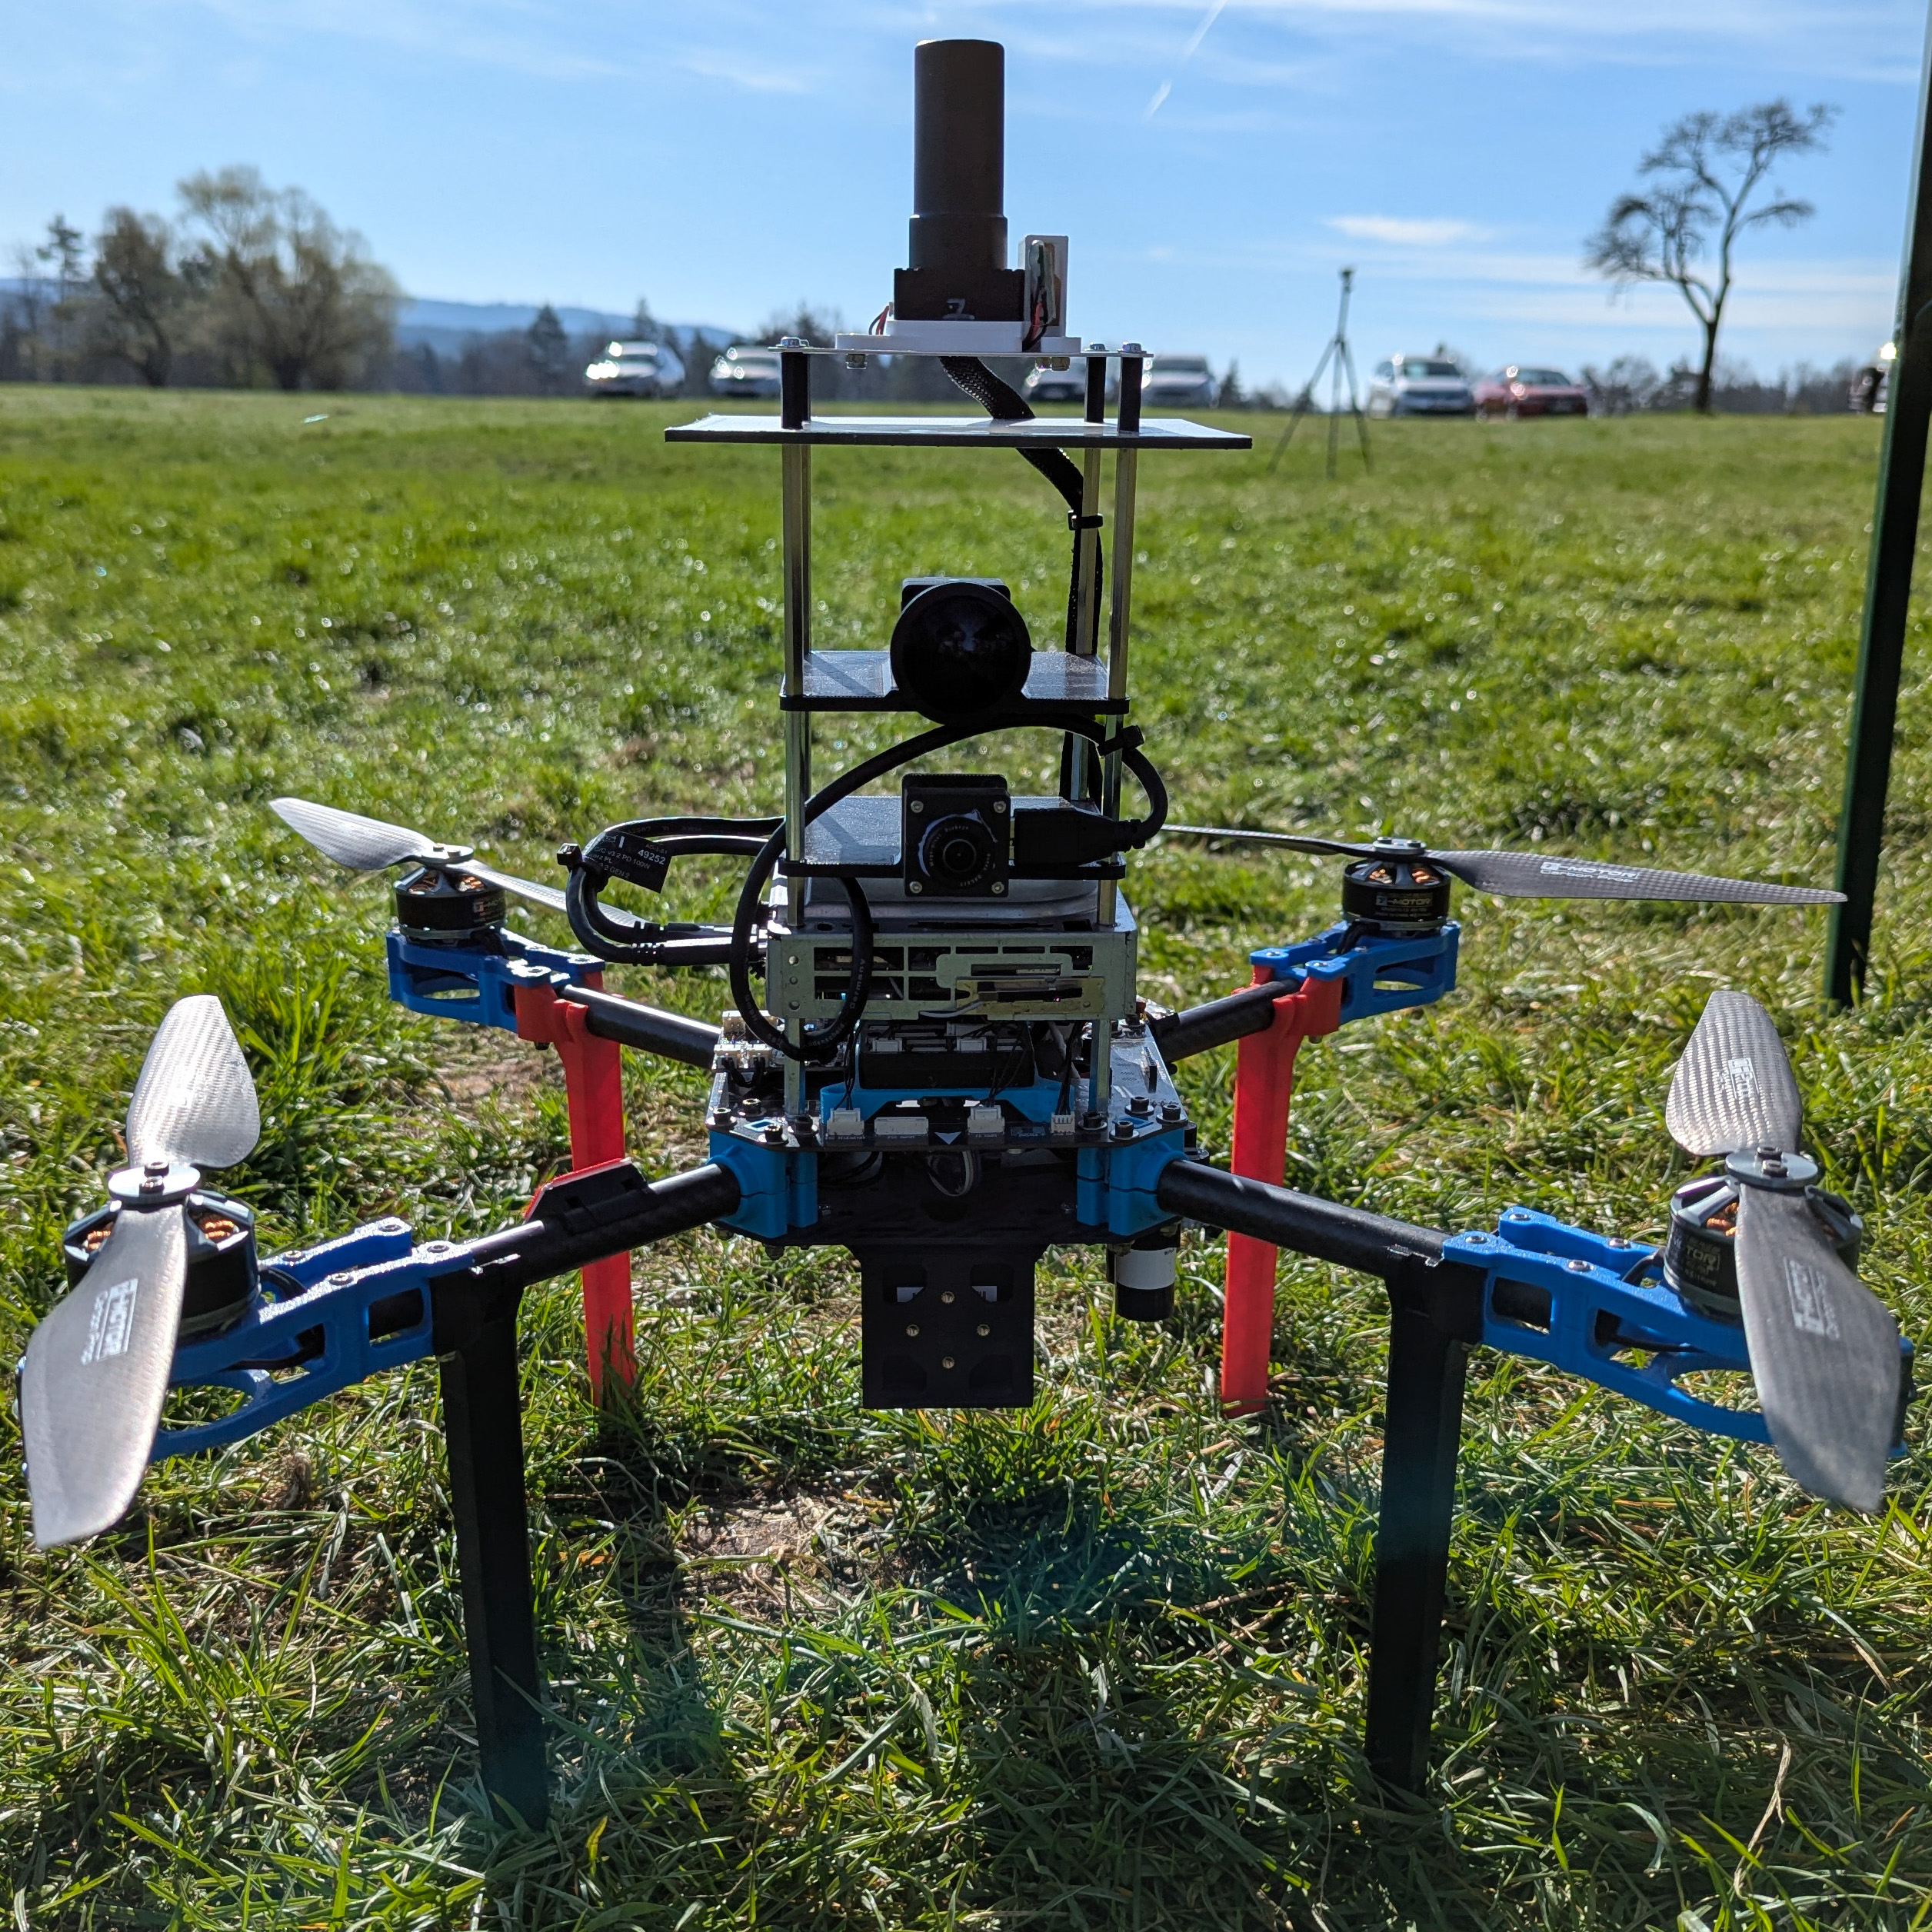
\includegraphics[width=0.4\textwidth]{./fig/photos/uav33.jpg}
	  \label{fig:uav33}
	}
	\subfloat[UAV37] {
	  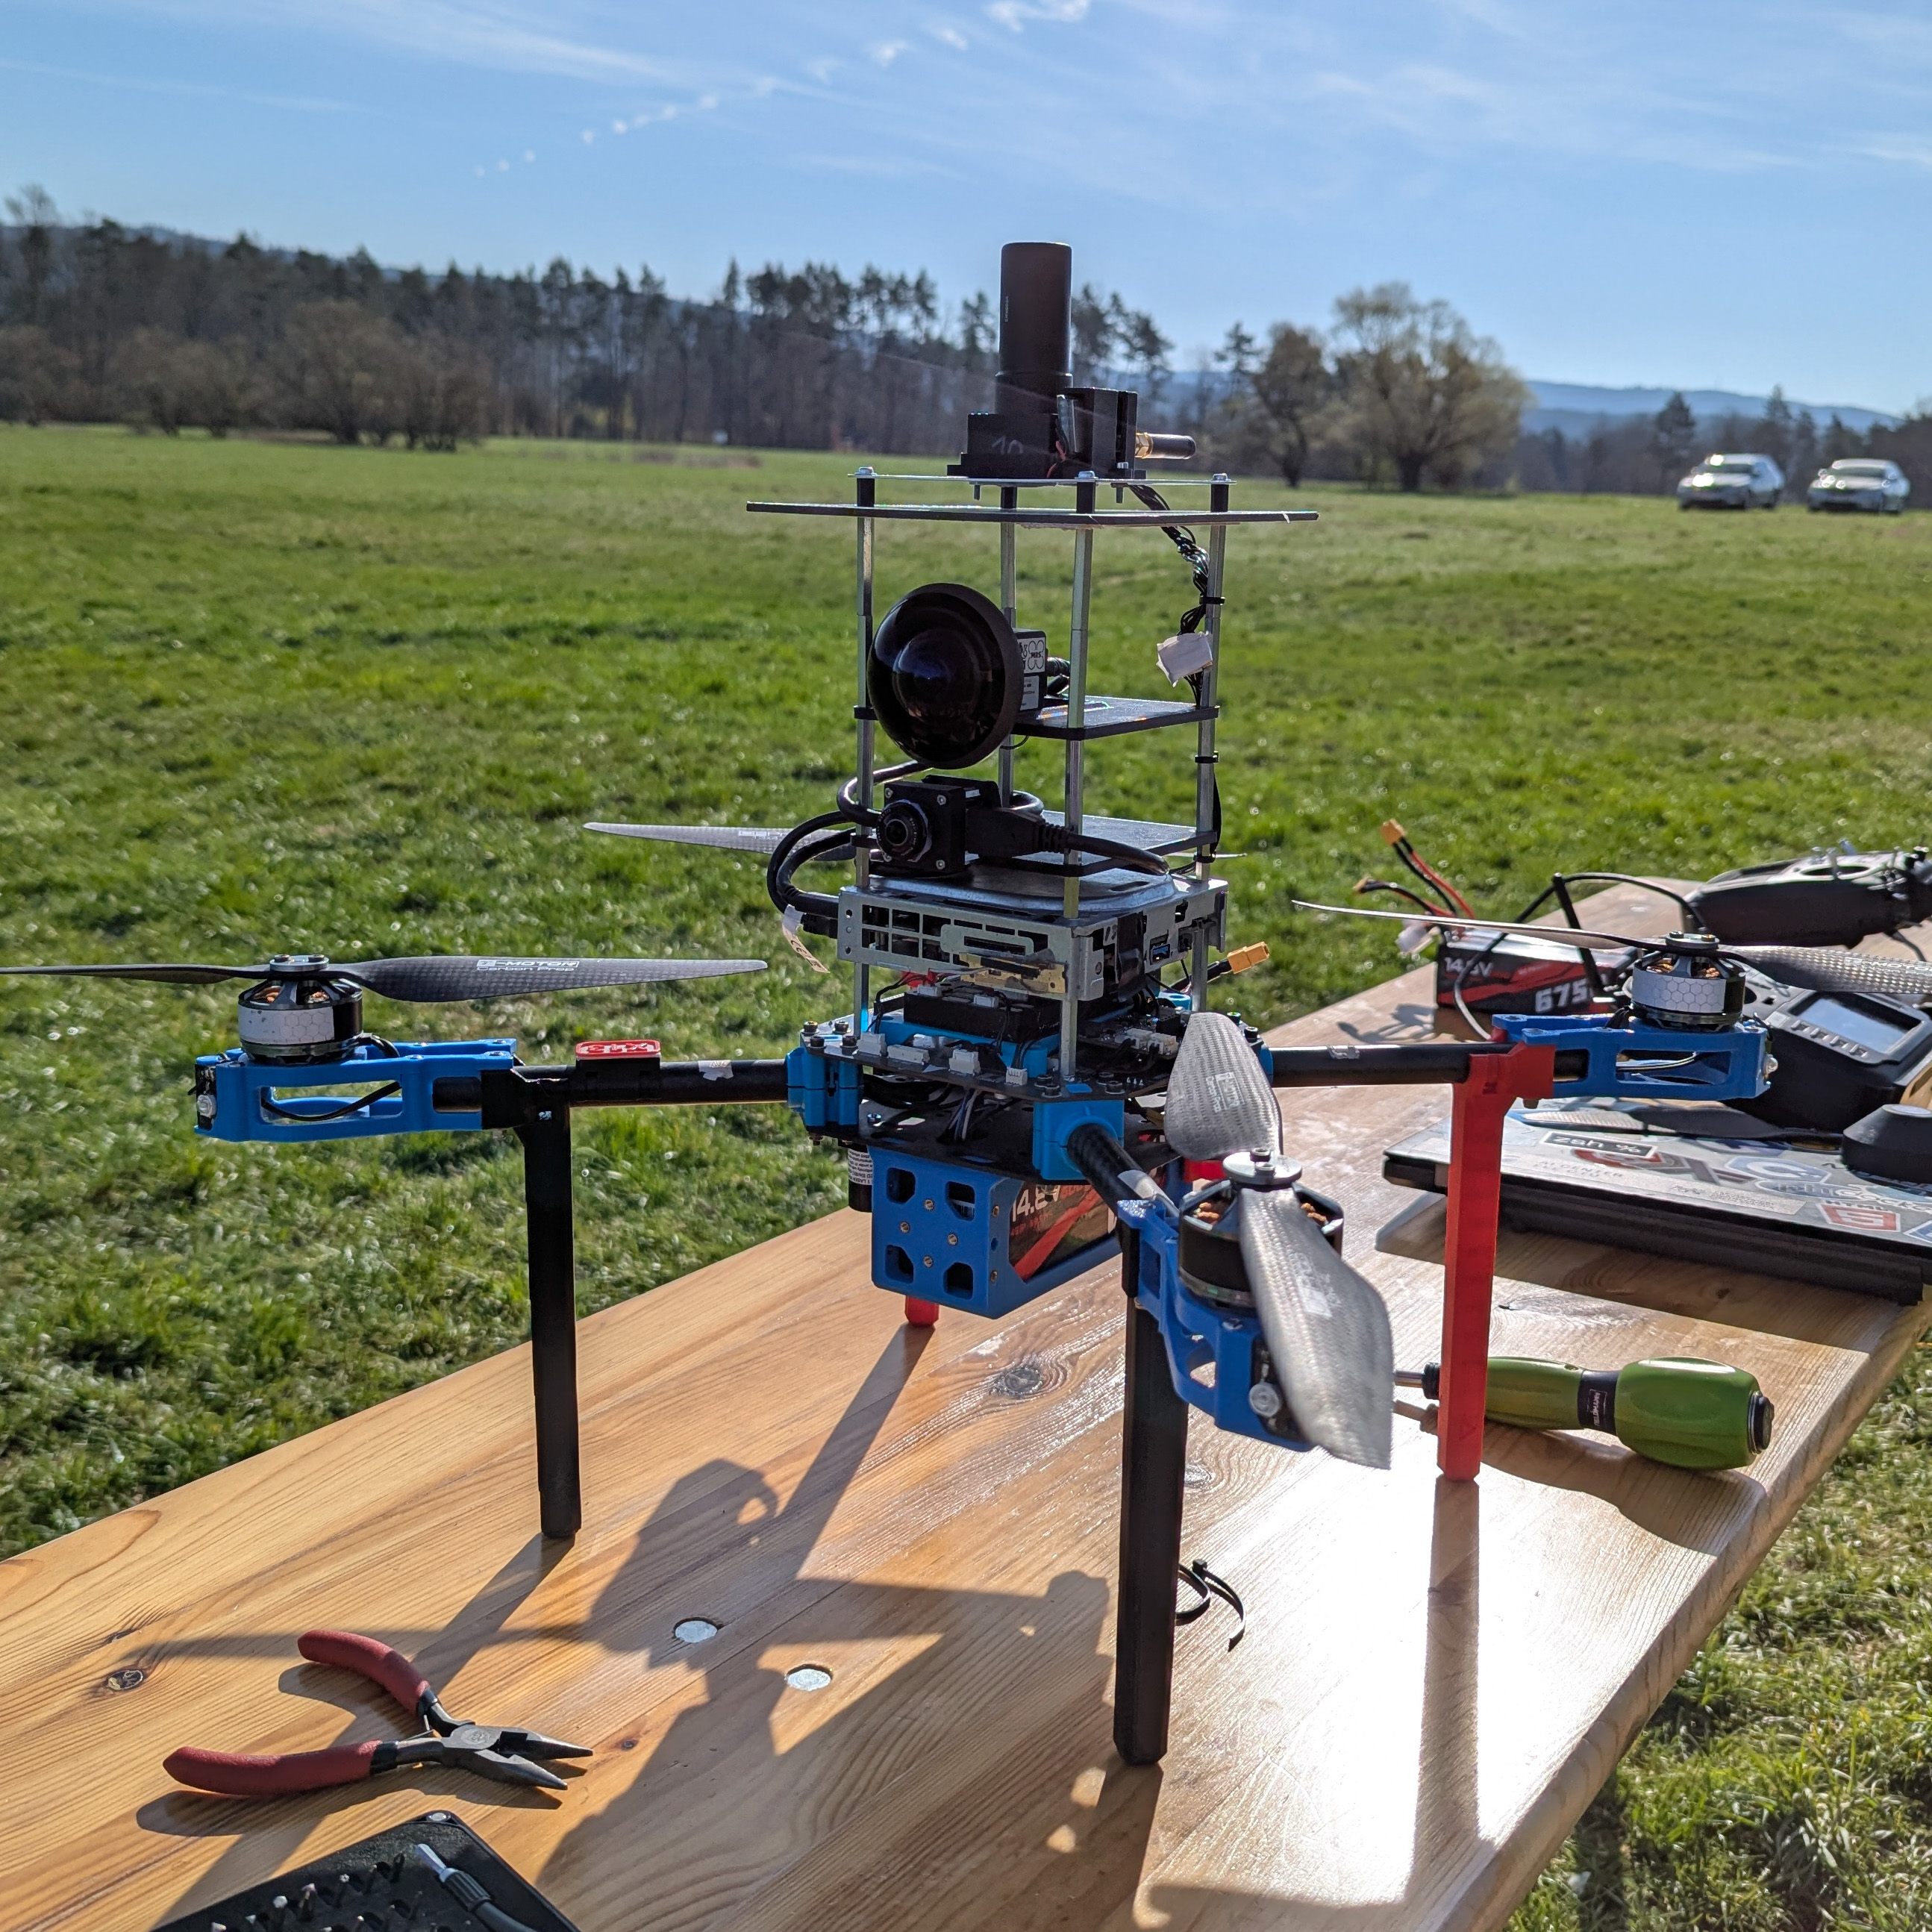
\includegraphics[width=0.4\textwidth]{./fig/photos/uav37.jpg}
	  \label{fig:uav37}
	}
	\caption{
		Two X500 UAVs, UAV33 on \reffig{fig:uav33} and UAV37 on \reffig{fig:uav37}.
  }
	\label{fig:uav33_37}
\end{figure}
Two pilots manually controlled the \ac{UAV}s, systematically varying the distance and angles between them to generate diverse measurement data during the experiment. All in-flight data, including sensor measurements and camera streams, we recorden in a \ac{ROS} bag file for subsequent analysis
in a simulated environment. In addition, raw event stream data from the event-based camera was also recorded and saved. The camera view from the UAV33
can be seen on \reffig{fig:exp1}. During the recording about $17$ million events were generated every second by each camera, which equates to a data
throughput of about $45$ MB per second per drone. Each raw recording is about $14$ gigabytes in size.

\begin{figure}[H]
	\centering
	\subfloat[Event-based camera output] {
	  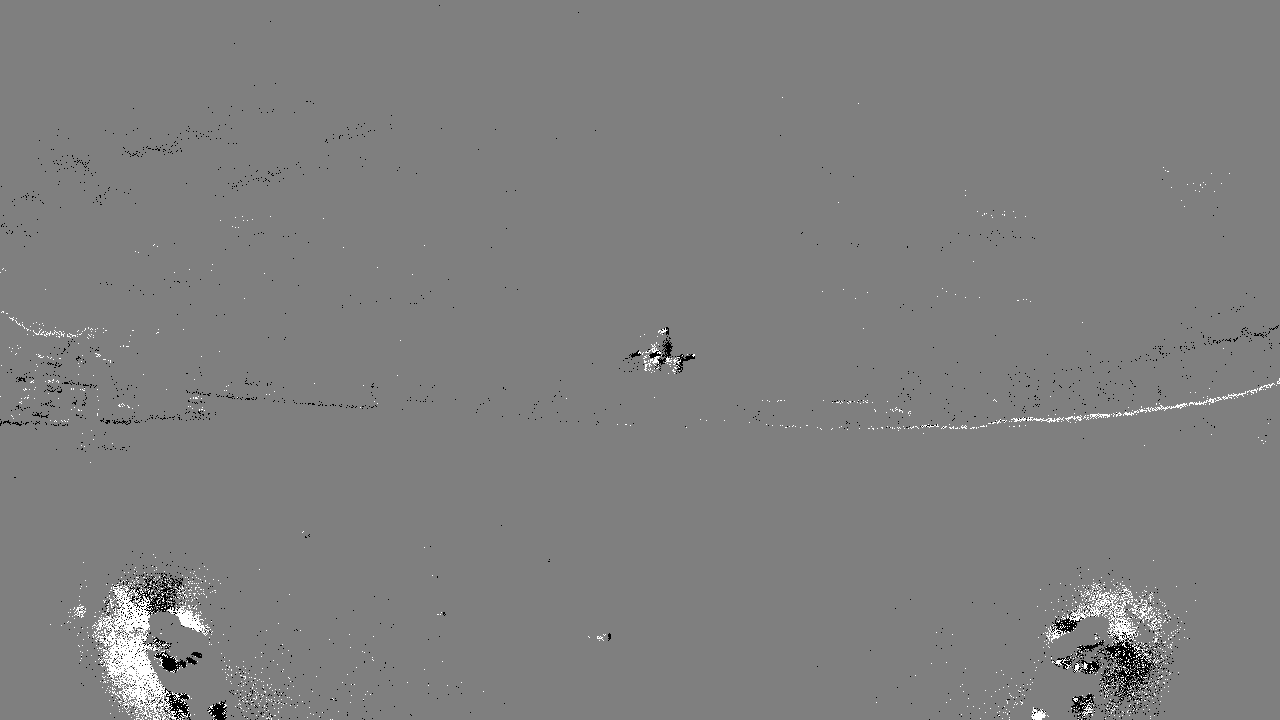
\includegraphics[width=0.50\textwidth]{./fig/photos/uav33_event.png}
	  \label{fig:exp1_event}
	}
	\subfloat[Basler camera output] {
	  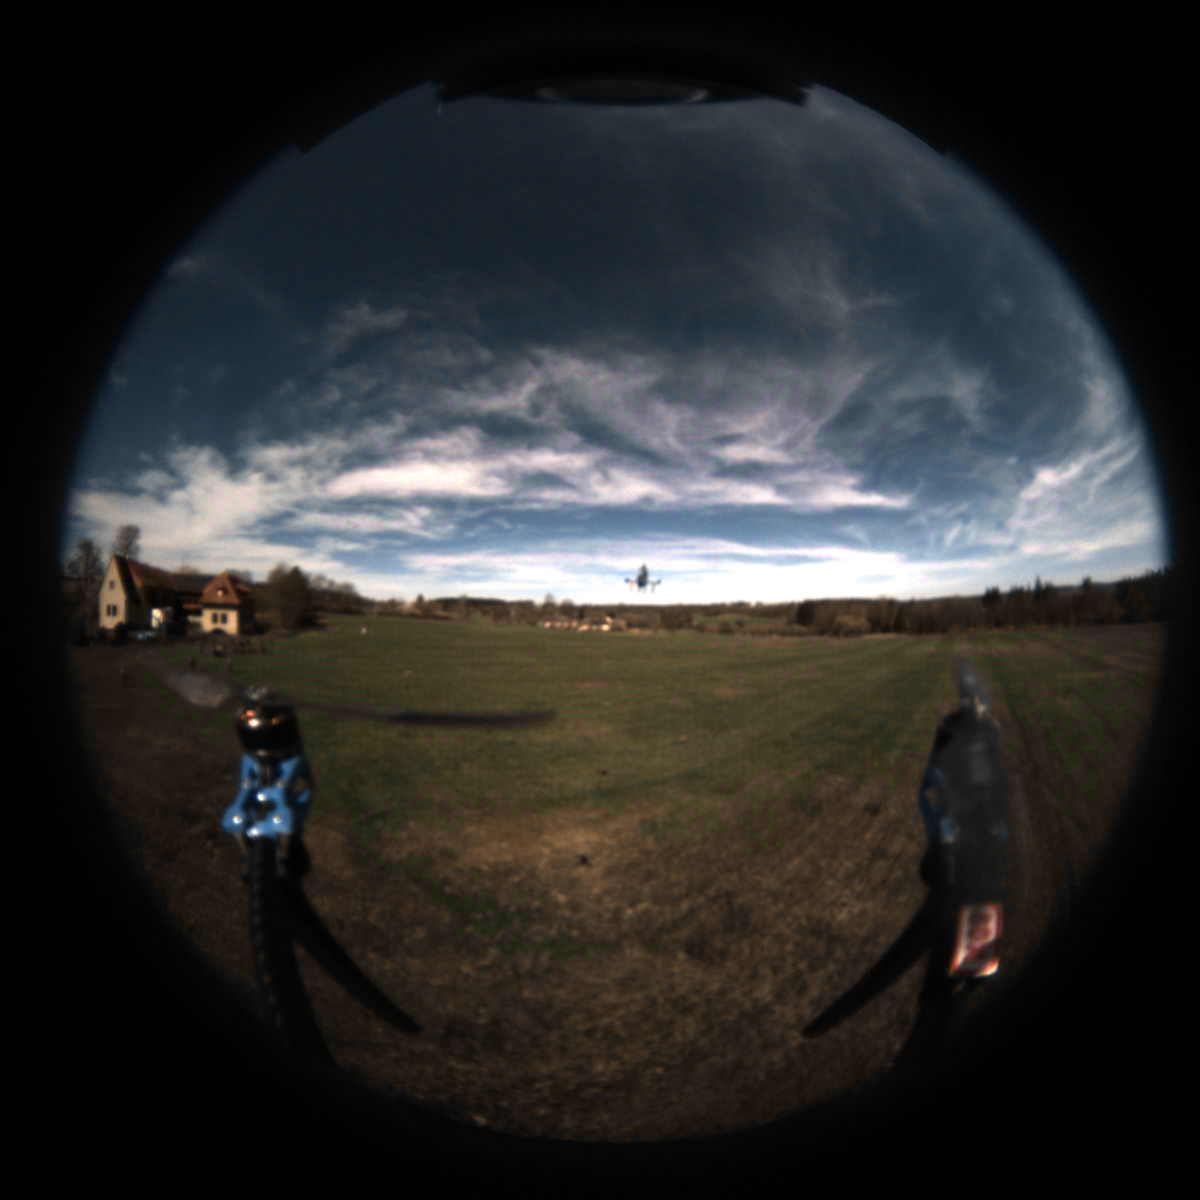
\includegraphics[width=0.282\textwidth]{./fig/photos/uav33_basler.png}
	  \label{fig:exp1_basler}
	}
	\caption{
		The view of the experiment from UAV33, with event data on \reffig{fig:exp1_event} and Basler camera view on \reffig{fig:exp1_basler}.
  }
	\label{fig:exp1}
\end{figure}

%\todo{SHOW MEASURED DATA FROM RQT}

%\todo{SHOW GNSS/ESTIMATION DIFFERENCES}

%\todo{SHOW THE RVIZ/RQTPLOT VISUALIZATION PIPELINE}

\section{Analysis}

The data was analyzed after the recording, by generating image frames from the raw event recordings. This data,
as seen on \reffig{fig:labeled}, has then been manually labeled and with the use of a blob detector the \ac{LED} sources
were selected.
\todo{maybe write more}

\begin{figure}[H]
	\centering
	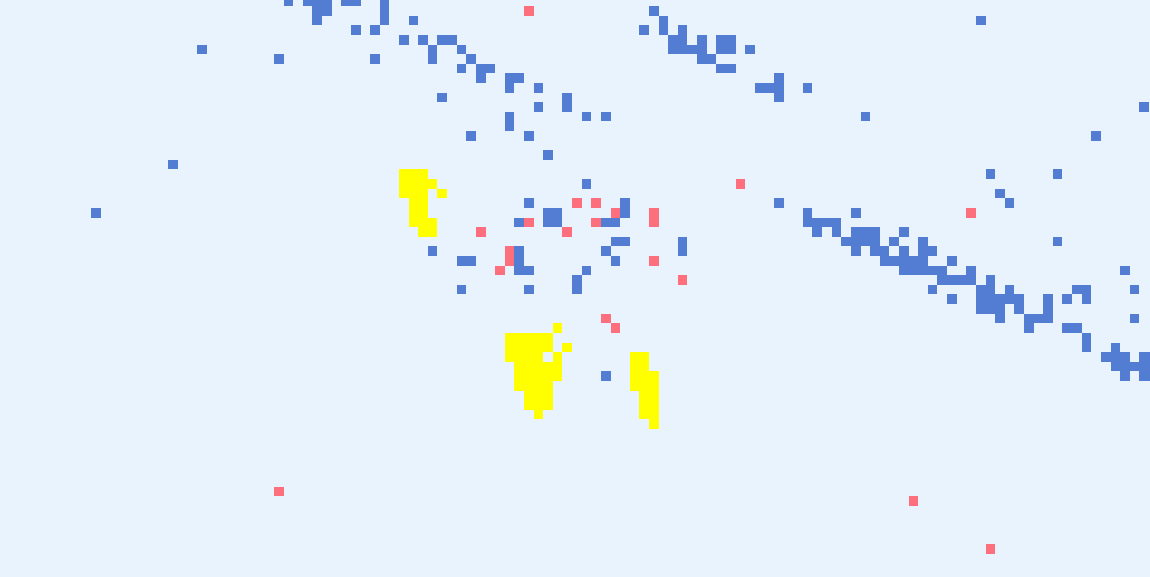
\includegraphics[width=0.7\textwidth]{./fig/photos/labeled_2.png}
	\caption{Labeled blob centers}
	\label{fig:labeled}
\end{figure}

\section{Experiment results}

For each labeled group of points a distance estimation was performed using the \texttt{DistanceEstimator} using the
\ac{P3P} algorithm. For each estimated pose, a distance from the camera was calculated, which was then compared to the
ground truth distance obtained from the \ac{GNSS}. The distance is calculated as a norm of the difference of the \ac{UAV} positions.
The results demostrate, that our approach achieves a mean absolute error of $2.47$ meters, with a standard deviation of $1.75$ meters,
indicating moderate precision under the experiment conditions.
The estimation
results can be seen on \reffig{fig:experiment_results}

\begin{figure}[H]
	\centering
	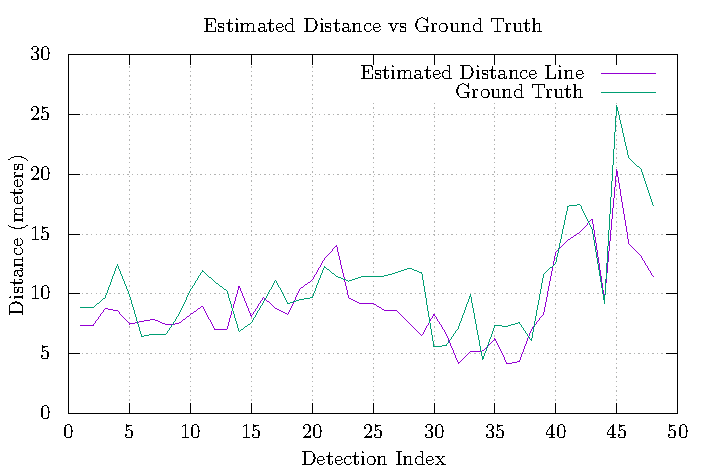
\includegraphics[width=0.7\textwidth]{./fig/tikz/experiment_analysis.pdf}
	\caption{The distance estimation data from the experiment, compared with the recorded GNSS data used as ground truth}
	\label{fig:experiment_results}
\end{figure}

\section{Real life deployment - estimation challenges}

The analysis presents several challenges, one of them being the identification of the moving \ac{UAV} in the recorded
data. The ideal solution is to identify which pixels are being generated with their specific frequeny, which the \ac{LED}
markers are set to blink on the. Sadly, during the measurement of our experiment, the \ac{UAV} produced a lot
of vibration in the data, which interfered with our measurements, and thus the detection of blobs has become a large obsacle.
When we generate images from the recording, the problem persists; How do we identify the correct blobs automatically, when
the \ac{UAV} can be at an arbitrary distance and orientation?
Manual labeling is not the definitive answer to our problem either because even the blob center selection itself can greatly
influence the estimation precision. In \reffig{fig:blob_comb}, we select a single pixel from each blob and run the distance estimation
for each combination of pixel. As we can observe, even a change in the range of 3 pixels can change the estimated distance by
$1.5$ meters. The center of a blob may be calculated as a geometrical center of the blob's pixels, but this approach fails
when the blob contains pixels which do not belong to them.
%Secondly, the calculation of the exact center would most likely yield results with sub-pixel level precision, requiring the placement of the center between the pixels

%As we have shown in \reffig{fig:labeled}, there exist a challenge of \ac{UAV} identification 
\begin{figure}[H]
	\centering
	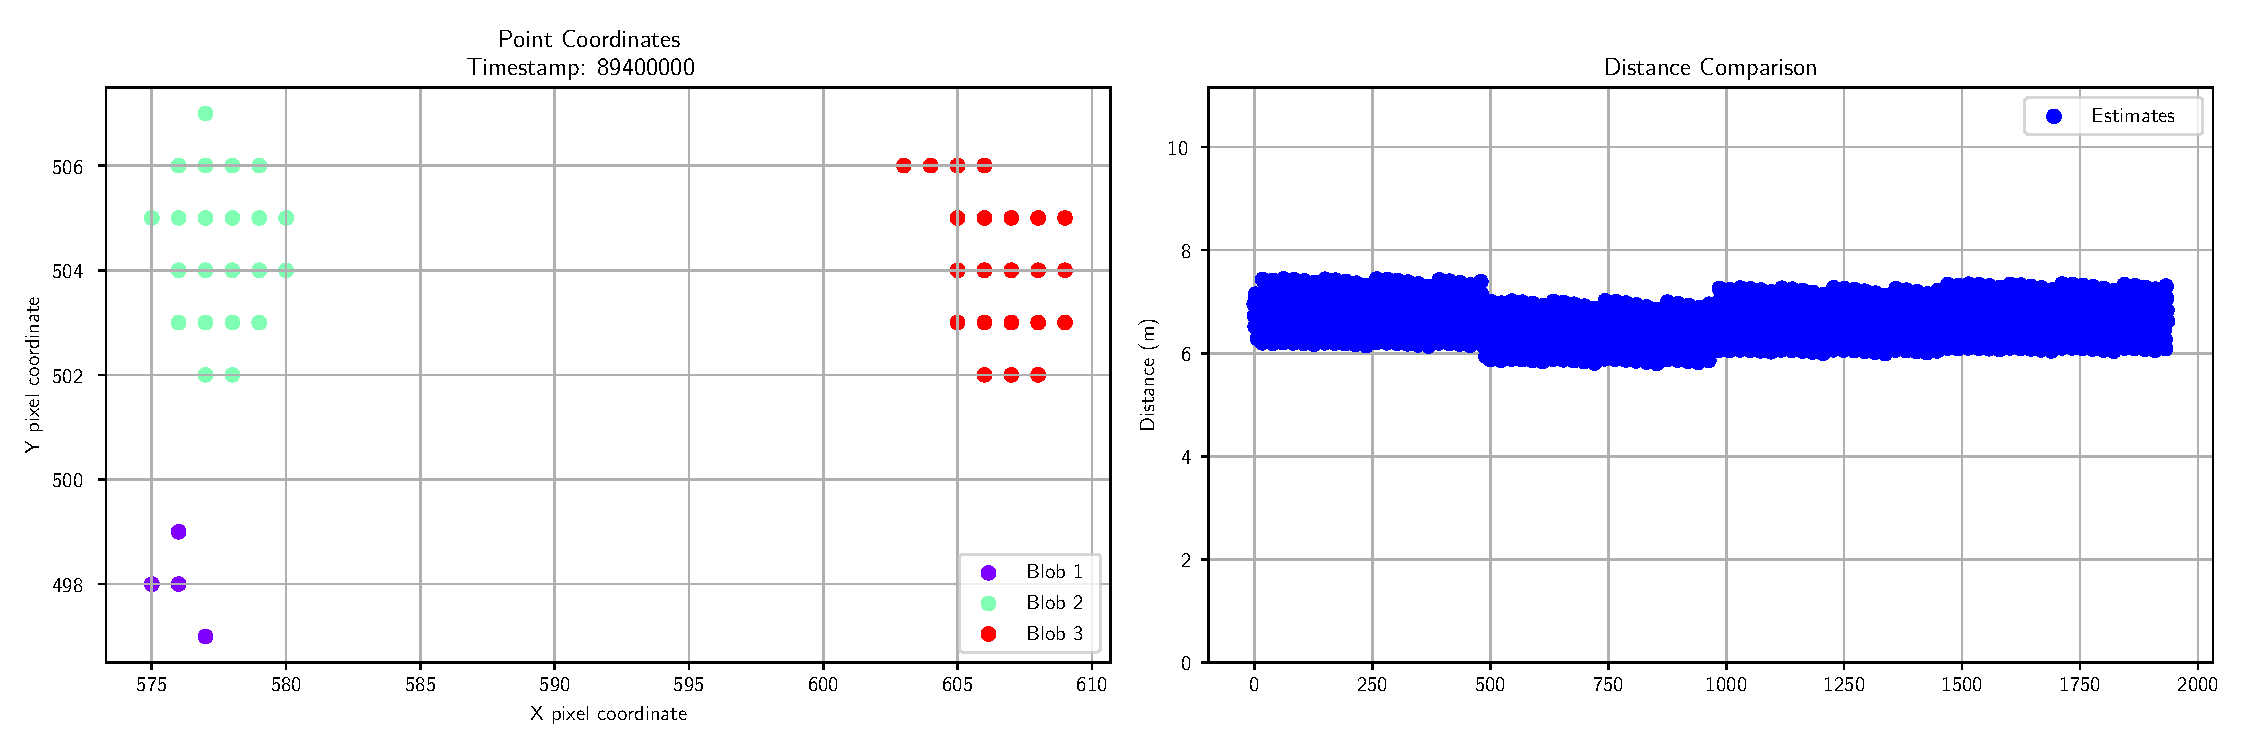
\includegraphics[width=0.99\textwidth]{./fig/pgfplot/estimation_selection_1.pdf}
	\caption{Blob centers with the resulting distance estimations for any combination of center selection}
	\label{fig:blob_comb}
\end{figure}

A fundamental limitation of any vision‐based positioning system is the finite spatial resolution of the camera sensor. As the distance to the \ac{LED}s increases, beyond roughly $20$ m in our setup, their angular size on the image plane decreases to just a few pixels. Once a marker spans only a few sensor pixels, adjacent light sources can begin to merge: individual \ac{LED} spots can no longer be differentiated and their point-spread functions overlap. This blending of pixel responses prevents the reliable separation of each \ac{LED} signal and ultimately makes accurate detection and decoding impossible.

%% --------------------------------------------------------------
%% |                         Conclusion                         |
%% --------------------------------------------------------------

%!TEX root = ../main.tex

\chapter{Conclusion\label{chap:conclusion}}
In this thesis, the response of an event-based camera to a modulated source of light (a \ac{UV} \ac{LED}) was discussed.
It was shown how the changing frequency, distance, and incidence angle influenced the average number of events generated by the camera.
The calibration method for fisheye lenses by Scaramuzza et al.~\cite{scaramuzzacalibration} was then discussed, which, in our cases,
utilized an LED lattice target instead of the normally used checkerboard image pattern.

Distance estimation was performed using the \ac{P3P} algorithm, which estimated the rotation and translation of a known
arrangement of 3D locations using their image coordinates. A stationary data set was collected and analyzed with this
approach, which has shown a median distance estimation error of $0.34$ meters with a standard deviation of $0.16$ meters.
A \texttt{DistanceEstimator} node was implemented in \ac{ROS}, which eased the distance estimation by subscribing
to detected \ac{LED} locations and publishing the estimated pose and distance.

This approach was used in our real-life experiment, where data was collected from two flying \ac{UAV}s, which were manually controlled by two pilots.
The data was then analyzed afterward, by manually marking the \ac{LED} locations. The resulting estimate has shown
higher errors (a mean absolute error of 2.47 meters with a standard deviation of 1.75 meters), compared to the statically measured data set,
due to the increased distance during flight and physical limitations of the methods and equipment used.

\section{Future work}
In the future, the detection of the \ac{LED}s is planned to be automated, enabling real-time distance and pose estimation.
This could be achieved by incorporating a robust feature detection algorithm or a machine learning-based object detection
algorithm into the pipeline.
A method using \ac{RSSR} for the improvement of the pose estimation could also be used to further improve pose estimation precision,
which was not further explored in this thesis, as for the inconclusive results obtained during the trial analysis of the data measured for this method and the lack of time for further research.

%% --------------------------------------------------------------
%% |                         References                         |
%% --------------------------------------------------------------

\chapter{References}

\printbibliography[heading=none,title={}]

%% --------------------------------------------------------------
%% |                         Appendices                         |
%% --------------------------------------------------------------

\appendix
\renewcommand\chaptername{Appendix}

\renewcommand{\thechapter}{A}
\renewcommand\chaptername{Appendix A}

\chapter{Appendix A}

\end{document}
